% ============================================================
%  GIST: Groundwater Interpolation in Space and Time
%  Master Thesis — BHT Berlin, Data Science
%  Robert Wienröder, 2026
% ============================================================
\documentclass[
  a4paper,
  oneside,
  11pt,
  parskip=half,
  headings=normal,
]{scrreprt}

% --- Encoding & Language ---
\usepackage[T1]{fontenc}
\usepackage[utf8]{inputenc}
\usepackage[english]{babel}

% --- Page Layout ---
\usepackage[
  top=2.5cm, bottom=2.5cm,
  left=2.5cm, right=2.5cm
]{geometry}

% --- Line Spacing ---
\usepackage{setspace}
\setstretch{1.25}

% --- Font ---
\usepackage{lmodern}

% --- Math ---
\usepackage{amsmath, amssymb, mathtools}

% --- Graphics ---
\usepackage{graphicx}
\usepackage{caption}
\usepackage{subcaption}
\graphicspath{{figures/}}

% --- Tables ---
\usepackage{booktabs}
\usepackage{tabularx}
\usepackage{longtable}
\usepackage{multirow}

% --- Units ---
\usepackage{siunitx}
\sisetup{detect-all, locale=US}

% --- Code Listings ---
\usepackage{listings}
\usepackage{scrhack}
\lstset{
  basicstyle=\ttfamily\small,
  breaklines=true,
  frame=single,
  numbers=left,
  numberstyle=\tiny,
}

% --- Colors (load before tikz/tcolorbox to avoid option clash) ---
\usepackage[dvipsnames]{xcolor}
\definecolor{citeblue}{RGB}{0,90,130}

% --- TikZ (for pipeline diagram) ---
\usepackage{tikz}
\usetikzlibrary{shapes.geometric, arrows.meta, positioning, fit, calc}

% --- Bibliography ---
\usepackage[
  backend=biber,
  style=authoryear,
  natbib=true,
  maxcitenames=2,
  maxbibnames=99,
  doi=true,
  url=true,
  isbn=false,
]{biblatex}
\addbibresource{bib/references.bib}
\AtEveryBibitem{\clearfield{urlyear}\clearfield{urlmonth}\clearfield{urlday}}

% --- Quotes ---
\usepackage{csquotes}

% --- Hyperlinks (load last) ---
\usepackage[
  colorlinks=true,
  linkcolor=black,
  citecolor=citeblue,
  urlcolor=MidnightBlue,
]{hyperref}
\usepackage[capitalise, noabbrev]{cleveref}

% --- Algorithms / Pseudocode ---
\usepackage{algorithm}
\usepackage{algpseudocode}

% --- Float placement ---
\usepackage{float}

% --- Misc ---
\usepackage{microtype}
\usepackage{enumitem}
\usepackage[most]{tcolorbox}
\tcbset{
  researchquestion/.style={
    colback=gray!8,
    colframe=gray!45,
    boxrule=0.5pt,
    arc=2pt,
    left=8pt, right=8pt,
    top=6pt, bottom=6pt,
    before skip=\baselineskip,
    after skip=\baselineskip,
  }
}

% --- Placeholder commands ---
\newcommand{\todo}[1]{{\color{red}\textbf{[#1]}}}

% ============================================================
%  Title Page Info
% ============================================================
\newcommand{\thesistitle}{Spatio-Temporal Interpolations \\for Global Groundwater Forecasts}
\newcommand{\theauthor}{Robert Wienr{\"o}der}
\newcommand{\thematrikel}{942815}
\newcommand{\thesupervisor}{\textbf{Prof.\ Dr.\ rer.\ nat.\ Felix Bie\ss{}mann}}
\newcommand{\thesecondreviewer}{\textbf{Prof. Dr. Patrick Erdelt}}
\newcommand{\thedate}{May 27, 2026}

% ============================================================
\begin{document}

\hypersetup{pageanchor=false}
\begin{titlepage}
  \centering
  \vspace*{2cm}

  {\Large Berliner Hochschule für Technik (BHT)}\\[0.3cm]
  {\large Department of Computing and Media}\\[0.3cm]
  {\large Master of Science in Data Science}\\[0.2cm]
  {\normalsize BHT Berlin and Cognitive Algorithms Lab, Berlin, Germany}\\[0.1cm]
  {\normalsize in collaboration with}\\[0.1cm]
  {\normalsize Lawrence Berkeley National Laboratory, Berkeley, California, USA}\\[0.1cm]
  {\normalsize and Federal Institute for Geosciences and Natural Resources (BGR), Berlin, Germany}

  \vspace{1.5cm}

  \rule{\textwidth}{1pt}\\[0.4cm]
  {\LARGE \textbf{\thesistitle}}\\[0.3cm]
  \rule{\textwidth}{1pt}

  \vspace{1.5cm}

  {\large Master Thesis}\\[0.5cm]
  submitted by\\[0.3cm]
  {\Large \textbf{\theauthor}}\\[0.2cm]
  Matriculation Number: \thematrikel

  \vspace{1.5cm}

  \begin{tabular}{ll}
    First Supervisor:  & \thesupervisor      \\[0.2cm]
    Second Reviewer:   & \thesecondreviewer  \\
  \end{tabular}

  \vfill

  Berlin and Berkeley\\
  \thedate

\end{titlepage}

\hypersetup{pageanchor=true}

\pagenumbering{roman}

\chapter*{Abstract}
\addcontentsline{toc}{chapter}{Abstract}

Groundwater monitoring networks cover only a fraction of the locations where predictions are needed, and most forecasting systems work only where wells already exist.
Forecasting groundwater levels (GWL) at existing monitoring wells improves considerably with
deep learning. However, predicting GWL at entirely unmonitored locations without any
historical observations is more difficult and receives less attention. Most
existing approaches do not test against large, fixed test sets of spatially separated
wells and therefore cannot "forecast anywhere".

This thesis introduces GIST (\textbf{G}roundwater \textbf{I}nterpolation in \textbf{S}pace
and \textbf{T}ime), a spatiotemporal pipeline combining a temporal and a spatial modeling component,
covering 1{,}040 monitoring wells across Brandenburg, Germany.
A Gated Recurrent Unit (GRU) produces temporal forecasts at monitored wells, which a Gaussian Process
(GP) then interpolates to locations excluded from training to simulate unmonitored locations.

The GRU matches the performance of a much larger Temporal Fusion Transformer baseline while
training roughly 90 times faster, which makes the full experimental setup feasible. One of the main findings is that temporal forecast quality is not the bottleneck
in the spatiotemporal pipeline: interpolating the actual observations at training wells instead
of the temporal predictions does not improve the error of the full spatiotemporal pipeline. The limiting factor is therefore spatial generalization, not temporal forecast quality. Distance to the nearest training 
well is the strongest predictor of per-well error. A jointly trained model combining GRU and GP with a combined loss does not improve overall performance but specifically reduces error for the most spatially isolated wells,
which are the hardest cases for a ``forecast anywhere'' system.
Together, these results demonstrate the feasibility of spatiotemporal GWL forecasting at unmonitored locations and show that further progress mainly depends on improving spatial generalization.


% \include{chapters/00_summary}

\chapter*{Acknowledgments}
\addcontentsline{toc}{chapter}{Acknowledgments}

First and foremost, I would like to thank my supervisors, 
Prof.\ Felix Bie\ss{}mann (BHT Berlin and Cognitive Algorithms Lab) 
and Dr.\ Charuleka Varadharajan (Earth and Environmental Sciences Area, 
Lawrence Berkeley National Laboratory, supported by the Laboratory 
Directed Research and Development program), for their guidance, 
support, and encouragement throughout this thesis.

I also thank Stefan Broda of the Federal Institute for Geosciences
and Natural Resources (BGR, Berlin) for his collaboration and
expert contributions to this work, and Maria Wetzel and Stefan Kunz
of BGR for their further contributions.

Vipin Singh and Nicholas Chandler of the 
Cognitive Algorithms Lab provided helpful input and discussions, 
and the entire team of Charuleka Varadharajan at the 
Earth and Environmental Sciences Area (EESA) of Lawrence Berkeley 
National Laboratory gave valuable feedback.

I am grateful to the Berliner Hochschule f{\"u}r Technik (BHT Berlin), and in particular 
to Prof.\ Stefan Edlich, Program Director of the M.Sc.\ Data Science 
program, for always being there for his students.

Special thanks go to the University of California, Berkeley, for 
the opportunity to study and conduct research there, and to
Prof.\ Michael Mahoney of the Department of Statistics 
at UC Berkeley, who hosted me in his graduate research class, which
made it possible for me to conduct this work while being 
affiliated with both UC Berkeley and the Earth and Environmental 
Sciences Area at Lawrence Berkeley National Laboratory, where he also
has an appointment.

This entire project would not have been possible without the initiative
of Prof.\ Felix Bie\ss{}mann, who originally established the connection
to Lawrence Berkeley National Laboratory. I also thank him
for his support in presenting this work at two international 
conferences (HydroML at the University of Texas at Austin and 
Groundwater Modeling and More at Princeton University), particularly
for his efforts in securing funding for travel, accommodation, and 
registration through the German Research Foundation (DFG) via 
BHT Berlin. In that context, I am also grateful to Charuleka Varadharajan 
and  Stefan Broda for encouraging and supporting my participation in 
these conferences.

Finally, I express my gratitude for the financial support of the German 
Academic Exchange Service (DAAD) through the HAW International
scholarship, which made it possible for me to complete this 
thesis in Berkeley.


\tableofcontents

\cleardoublepage
\pagenumbering{arabic}

% Chapter 1 — Introduction
% !TEX root = ../main.tex
\chapter{Introduction}
\label{ch:introduction}

Groundwater supplies water for drinking, agriculture, and ecosystems worldwide \citep{taylor2013groundwater},
but monitoring networks cover only a fraction of the areas that depend on it.
The German state of Brandenburg is characterized by a continental climate,
low annual precipitation (500--700\,mm \citep{dwd2024klimaatlas}), declining groundwater recharge \citep{francke2025groundwater}, and
extensive agricultural (49\%) and forested (35\%) land \citep{statistikbb2023}. 
Since both agriculture and forests rely heavily on groundwater, and the low 
precipitation limits natural recharge, groundwater availability is
crucial for agricultural productivity and forest health. Reliable groundwater level (GWL) forecasts
are therefore essential for farmers, authorities, land managers, and planners.

The Brandenburg State Office for the Environment (LfU) operates a dense network of over 2{,}100
monitoring wells \citep{lfu2024styx}, of which 1{,}040 remain after quality filtering. The wells are recording weekly 
GWL observations that span more than seven decades. These wells are spread across 
Brandenburg's full territory but naturally cannot provide continuous spatial coverage,
which leaves the vast majority of areas effectively unmonitored. The key 
challenge this thesis deals with is:

\begin{tcolorbox}[researchquestion]
Given past groundwater level observations at monitored well locations,
can we reliably predict groundwater levels at unmonitored locations at future
horizons?
\end{tcolorbox}

The long-term goal is reliable forecasting at unmonitored locations, in other words
a ``forecast anywhere'' system.

For Brandenburg's farmers, foresters, and water managers, knowing what the groundwater level will do over the next few weeks at their specific location naturally matters more than knowing what it does at the nearest monitoring well. Decisions about irrigation scheduling, emergency groundwater pumping during drought, and long-term land management all depend on local conditions. The LfU network is dense by any standard, but roughly 2{,}100 wells (of which 1{,}040 meet the quality criteria for this study) still cannot cover 29{,}654\,km$^2$ continuously. A practical ``forecast-anywhere'' deployment requires reliable GWL estimation at any point in the state on demand.

This problem has two dimensions:

\begin{description}
  \item[Temporal] Predicting future GWL at a well given its history and input features
  \item[Spatial] Interpolating temporal GWL forecasts to a location where no observations exist
\end{description}

Handling both simultaneously, and therefore predicting GWL at locations where no observations
exist, is the core challenge of spatiotemporal GWL forecast interpolation as formulated in this thesis.

\section{Problem Statement}
\label{sec:problem_statement}

Formally, the training data consist of time series $y_{i,t}$ of groundwater levels at wells 
$i \in \mathcal{W}_\text{train}$ for time steps $t = 1, \ldots, T$. Given a set of dynamic 
and static features, our goal is to predict the future GWL time series $\hat{y}_{j, t+1:t+H}$ at
test wells $j \in \mathcal{W}_\text{test}$, where $\mathcal{W}_\text{train} \cap
\mathcal{W}_\text{test} = \emptyset$. Forecasts are produced at all forecast horizons from 1 to $H = 16$ weeks ahead.

At the spatial training wells $\mathcal{W}_\text{train}$, the time series are further divided into a temporal training period, a validation period, and a temporal test period. The temporal test period also provides the true observations used by the true-observation interpolation baseline.

The key challenge that distinguishes this problem from standard time series forecasting is that 
the test wells are entirely unseen by the model during training. Spatial interpolation comes 
entirely from learned relationships between hydrogeological features and GWL dynamics.

\section{Contributions}
\label{sec:contributions}

Reliable spatiotemporal GWL estimation at unmonitored locations would matter for water management and drought response, but whether such estimation can be done reliably is not obvious. The spatial interpolation step could fail because temporal forecasts are too noisy, because the GP cannot generalize across the spatial structure of GWL in Brandenburg, or because no available hydrogeological feature carries enough information to bridge the gap between monitored and unmonitored locations. This thesis investigates these potential failure modes directly. That the GRU can match the TFT at a fraction of the training cost is not a contribution in isolation; it is what makes everything below possible. The contributions are:

\begin{enumerate}
  \item A \textbf{GRU sequence-to-sequence model} that matches the predictive performance of the
  Temporal Fusion Transformer of \citet{kunz2025} on the Brandenburg dataset while being nearly two
  orders of magnitude faster to train, which enables full hyperparameter optimization (HPO),
  feature ablation studies, multi-seed stability analysis, joint training runs, and a large
  number of preliminary experiments.

  \item An analysis of how \textbf{interpolation difficulty scales with spatial isolation}
  across 40 random split seeds, which shows that seeds drawing spatially isolated test wells
  are systematically harder to predict. This finding motivates the 40-seed evaluation design.

  \item A \textbf{spatiotemporal two-stage pipeline} (GRU for temporal forecasting, GP for
  spatial interpolation), evaluated under the co-location constraint on a \textbf{random 90/10
  split} of 104 test wells.

  \item A \textbf{GP feature ablation study} over 30 spatial feature configurations that
  shows hydrogeological zone to be the single most informative covariate for spatial
  interpolation, with no other feature or combination matching its performance on the main 90/10 random spatial split.

  \item An analysis of the \textbf{true-observation interpolation baseline} which replaces GRU predictions with
  true observations as GP input and shows that the gap between using
  true observations and GRU predictions as GP input is negligible, which means that temporal
  forecast quality is not the primary bottleneck for the spatiotemporal forecast interpolation problem.

  \item An analysis of \textbf{distance-dependent effects in jointly trained spatiotemporal
  modeling}: on average, end-to-end joint training of the temporal and spatial components does not outperform the two-stage pipeline,
  but for test wells more than roughly 4.5\,km from any training well the ranking reverses,
  which is the setting where the two-stage pipeline is least reliable.
\end{enumerate}

\section{Thesis Structure}
\label{sec:structure}

Chapter~\ref{ch:related_work} surveys prior work on deep learning for hydrology, GWL forecasting with machine learning, and spatial interpolation approaches. Chapter~\ref{ch:data} describes the Brandenburg monitoring network, the static and dynamic features used as model inputs, and the temporal and spatial structure of the data. Chapter~\ref{ch:methods} introduces the GRU and GP components, the spatiotemporal pipeline designs, and the evaluation protocol. Chapter~\ref{ch:results} reports the empirical findings. Chapter~\ref{ch:discussion} interprets the results, documents approaches that did not work, and discusses the limitations. Chapter~\ref{ch:conclusion} summarises and points to future work.

% Chapter 2 — Related Work
% !TEX root = ../main.tex
\chapter{Related Work}
\label{ch:related_work}

This chapter surveys the literature this thesis builds on, covering deep learning for hydrological forecasting
(\cref{sec:rw_dl_hydro}), groundwater level prediction with machine learning
(\cref{sec:rw_gwl}), prediction at spatially unmonitored locations
(\cref{sec:rw_ungauged}), spatial interpolation and Gaussian Process regression for
groundwater (\cref{sec:rw_gwl_interp}), joint spatiotemporal modeling
(\cref{sec:rw_joint}), uncertainty quantification (\cref{sec:rw_uq}), and
reproducibility practices in deep learning for hydrology (\cref{sec:rw_repro}). The chapter
closes with a dedicated discussion of the most directly related work, \citet{kunz2025}, and
the gaps this thesis fills (\cref{sec:rw_kunz}).

%-----------------------------------------------------------
\section{Deep Learning for Hydrological Forecasting}
\label{sec:rw_dl_hydro}
%-----------------------------------------------------------

Hydrological time series modeling has been dominated by recurrent neural
networks (RNNs). Long Short-Term Memory (LSTM) networks \citep{hochreiter1997long}
solved the vanishing gradient problem of early RNNs by introducing memory cells and
multiplicative gating mechanisms, which makes it possible for gradients to flow over
long sequences. This matters for hydrology, where groundwater and streamflow
dynamics show long-term patterns over weeks to months.
The Gated Recurrent Unit (GRU) \citep{cho2014learning} simplifies the LSTM design to two gates at lower computational cost, which makes it a practical alternative for the long look-back windows (52 weeks) required in this thesis.
Each GRU cell has its own reset and update gate, so cells can specialize across timescales:
cells that mostly keep their update gate active hold onto long-range patterns, while cells
that frequently reset respond to recent inputs. This makes the GRU a good fit for
groundwater dynamics, where precipitation responses are fast and seasonal recharge is slow.
\citet{willard2025ensembles} systematically evaluate GRUs for prediction at unmonitored
locations across a large set of stream temperature prediction tasks and find similar performance to LSTMs.

\citet{kratzert2018rainfall} show
that LSTMs trained on 241 catchments from the CAMELS (Catchment Attributes and Meteorology for Large-sample Studies) benchmark dataset can match or
exceed calibrated conceptual models (physics-based watershed models whose parameters are
fitted to observed streamflow at each individual site) for rainfall-runoff prediction. A key finding is that models trained jointly on groups of catchments can match separate models fitted to each catchment individually. The paper further shows
that LSTMs substantially outperform traditional RNNs in snow-influenced catchments: the RNN
cannot retain multi-month snow accumulation across winter because of vanishing gradients,
whereas the LSTM cell state stores this information without any explicit snow encoding. This thesis uses a GRU for the same reason: seasonal groundwater recharge also develops over months.

\citet{kratzert2019toward} extend this approach to the prediction-in-ungauged-basins (PUB) problem, which asks how to predict at basins with no observed streamflow, by feeding fixed catchment features into a global model, which lets it generalize to unseen sites without per-site training. They show that an LSTM trained on gauged basins can generalize to entirely withheld basins via static catchment attributes alone, outperforming calibrated physics-based models despite never training on those basins. The PUB problem is similar to the spatial interpolation challenge of
this thesis: just as PUB requires predicting streamflow at a site with no historical
observations, this thesis requires predicting groundwater levels at wells where no time series
has ever been recorded.

\citet{gauch2021rainfall} extend the global model idea to multi-timescale prediction, introducing a modified LSTM architecture that simultaneously generates predictions at daily and hourly temporal resolutions.

\citet{kratzert2024never} argue in a HESS Opinions piece that training on one basin at a time is statistically inferior: models then overfit to local patterns and miss the signal shared across sites. This thesis follows the same reasoning.

\citet{nearing2021role} argue that the success of DL for predicting at ungauged basins is a call to action for the hydrology community to develop quantitative, scale-relevant theories of watersheds alongside ML.

%-----------------------------------------------------------
\section{Groundwater Level Prediction with Machine Learning}
\label{sec:rw_gwl}
%-----------------------------------------------------------

Compared to surface water modeling, groundwater level prediction differs in a few ways: slower seasonal dynamics, strong coupling to geology and land use, and sparser
observational networks. \citet{heddam2022kriging} review over a hundred studies applying
feed-forward networks, SVMs, random forests, LSTMs, and hybrid models to GWL prediction
across diverse hydrogeological settings.
Most published work only evaluates on test time periods at monitored wells, so the harder problem of predicting at unmonitored locations is rarely addressed.

\citet{wunsch2021groundwater} systematically compare several neural architectures for GWL forecasting across a set of monitoring wells in the Upper Rhine Graben, spanning Germany and France.
NARX models outperform LSTM and CNN architectures on most metrics in both single-step and multi-step forecast settings, though for multi-step forecasting LSTMs and CNNs achieve higher R² scores.

\citet{heudorfer2024challenges} train a global LSTM conditioned on site-specific attributes on 108 monitoring wells
distributed across Germany, combining dynamic meteorological inputs with static site
attributes, and achieve a mean NSE above 0.8 in an in-sample setting, which is comparable to or better than single-well models trained separately on each location. Their study is
the direct predecessor to \citet{kunz2025}, which scales the approach to 5{,}288 wells using
TFT and N-HiTS architectures. The more informative result comes from their out-of-sample
evaluation, where entire wells are withheld from training: mean NSE drops to approximately
0.67--0.69 for models conditioned on static environmental or time-series features, while a
model with no static features at all achieves a mean NSE of 0.73, outperforming all
static-feature variants. Permutation importance shows that dynamic meteorological inputs matter by orders of magnitude more than any static feature.
Replacing all static features with random integers gives indistinguishable in-sample performance, which shows the model uses static features as well IDs to memorise each well's behaviour rather than learning patterns that transfer across locations. This is not specific to groundwater: \citet{lim2021temporal}
report the same for TFT across commercial forecasting datasets, where the unique ID for each time series consistently gets the highest importance score above all other static features.
Static attributes work in the rainfall-runoff literature, but do not seem to help for groundwater here, most likely because 108 wells is too few and too similar for any real correlations between static attributes and dynamics to show up. This is one reason this thesis adds a GP interpolation stage: static attributes alone are not enough to generalize to unmonitored locations.
\citet{willard2023time} mark the role of static site characteristics in ML models for
unmonitored prediction as an open question beyond groundwater, which
means the Heudorfer finding is not a groundwater-specific exception but part of a wider unresolved problem.

GWL dynamics differ from surface-water systems in two important ways. First,
groundwater responds slowly to precipitation: the subsurface introduces lags of weeks to months between precipitation events and aquifer response, which makes long look-back windows essential. The one-year look-back window used
in this thesis ($L = 52$ weeks) matches this delay. Second, the
spatial structure of GWL is shaped by geological heterogeneity, which cannot be
inferred from time series alone. This thesis handles it by encoding well-specific hydrogeological attributes into the GRU's initial hidden state through a linear projection layer.

\citet{ohmer2026nevertrain} find that global LSTM models match per-well models in accuracy across approximately 3{,}000 German monitoring wells, with accuracy depending more on training-well similarity to the target than on training-set size. This suggests the benefit of global training depends on how representative the training population is, a caveat relevant to this thesis.

The broader German groundwater monitoring context is documented in \citet{ohmer2026gemsger},
who compile a 32-year benchmark dataset (1991--2022) of 3{,}207 wells across Germany with
meteorological inputs and over 50 site-specific static attributes. The Brandenburg LfU
network used in this thesis is one component of this larger national infrastructure; this
dataset could be used to test the GIST pipeline across all of Germany.

%-----------------------------------------------------------
\section{Prediction at Unmonitored and Ungauged Locations}
\label{sec:rw_ungauged}
%-----------------------------------------------------------

Parameter regionalization approaches estimate model parameters for ungauged sites by using parameters of nearby gauged ones. Deep learning replaces this step with static-attribute conditioning: \citet{kratzert2019toward} show that a global model conditioned on site attributes can generalize to unseen sites without per-site training. This still assumes that static attributes are informative enough to characterize a new location's dynamics. For groundwater, this assumption can fail when the geological setting of the target wells is not well represented in the training data, which is one of the main challenges this thesis deals with.

\citet{li2022regionalization} extend the PUB approach by replacing static site attributes with randomly assigned embedding vectors and show that a global LSTM can represent
site-specific behavior at gauged sites without being given any physical information about the site. Their finding applies only to sites seen during training: random vectors carry no information about unseen locations and cannot support prediction at genuinely unmonitored wells.

\citet{willard2023time} survey ML techniques for time series prediction at unmonitored sites across streamflow, water quality, and lake temperature. Almost all reviewed studies address streamflow or water quality; groundwater appears only marginally, and \citet{kunz2025} is one of the few large-scale studies applying global deep learning to GWL prediction.

\citet{varadharajan2022machine} discuss ML applications and opportunities for river water quality prediction and identify spatial generalization to unmonitored locations as a key open challenge. \citet{heudorfer2024challenges} measure the same problem for groundwater models directly (see \cref{sec:rw_gwl}). Most of these studies use leave-one-out cross-validation, which retains close spatial neighbors in training and makes the task easier than realistic deployment; the spatial split design used here addresses this (\cref{sec:spatial_splits}).

%-----------------------------------------------------------
\section{Spatial Interpolation of Groundwater and Geostatistical Methods}
\label{sec:rw_gwl_interp}
%-----------------------------------------------------------

Spatial interpolation of GWL has a long history in hydrogeology, mainly through geostatistical methods. Ordinary kriging treats GWL as a spatially correlated random field (one where the correlation between any two measurement locations depends on their distance) and estimates the covariance structure from the empirical variogram, a function describing how correlation decays with distance \citep{rasmussen2006gaussian}.
Spatiotemporal extensions of kriging model GWL jointly over space and time. \citet{ruybal2019evaluation} show that spatiotemporal regression kriging outperforms ordinary spatial kriging for the sparsely sampled Arapahoe aquifer in Colorado: adding temporal correlation reduces prediction error at unmonitored times. \citet{kazemi2021evaluation} apply spatiotemporal regression kriging to the Harvey River Catchment in Western Australia and assess accuracy via leave-one-out cross-validation. \citet{junezferreira2023assessment} do the same for the Basin of Mexico aquifer and confirm that spatiotemporal interpolation yields smaller errors than independent spatial snapshots. In all three cases, leave-one-out cross-validation retains close spatial neighbors in training, which makes the task easier than it would be in a realistic deployment scenario \citep{roberts2017cross} (see also \cref{sec:rw_ungauged}).

Several recent studies combine machine learning with geostatistical methods. \citet{zowam2024} combine ML point predictions with empirical Bayesian kriging (a variant of kriging that estimates the variogram locally around each prediction point rather than fitting one global model) for predicting GWL changes across Arizona. Like this thesis, they evaluate on well locations that are excluded from training, rather than using the same locations at different time steps. The spatial test set is small (7 out of 59 wells), however, which limits how reliable the performance estimates are.

\citet{pradhan2024modeling} combine a deep neural network with a GP for GWL interpolation in California's Central Valley in an architecture similar to this thesis: the network learns a feature representation from lithological and hydrogeological inputs, and the GP interpolates in that space. Their comparison of a coordinate-only GP against a feature-augmented GP mirrors the feature ablation in this thesis. The main difference is that Pradhan et al.\ estimate fixed parameters of a simple trend model from past observations, without a temporal forecasting component. This thesis adds a GRU as the first stage and interpolates GRU predictions rather than observations.

GP regression is a Bayesian framework for spatial interpolation that gives both predictions and uncertainty estimates \citep{rasmussen2006gaussian}. A GP with a stationary kernel is mathematically equivalent to ordinary kriging: both estimate a spatial field using a covariance function that depends only on distance \citep{rasmussen2006gaussian}. The Matérn family of kernels is the standard choice in spatial statistics because it directly controls how smooth the predicted surface is; the Matérn-$\tfrac{3}{2}$ kernel assumes once-differentiable processes and is common for physical spatial fields \citep{rasmussen2006gaussian}. GP inputs can also include spatial features beyond coordinates (covariate-augmented kriging), and which features help is not obvious in advance.

%-----------------------------------------------------------
\section{Joint Spatiotemporal Models and Neural Processes}
\label{sec:rw_joint}
%-----------------------------------------------------------

Several models learn spatial and temporal patterns jointly in a single stage. This thesis also evaluates a jointly trained spatiotemporal model alongside the two-stage design.

Deep kernel learning \citep{wilson2016deep} replaces the fixed GP kernel with a neural network that maps inputs to a learned feature space, which gives the GP more flexibility to capture complex spatial patterns.

Neural Processes \citep{garnelo2018neural, dubois2020npf} encode a set of observations into a latent representation and predict at arbitrary query locations; in effect, they learn a distribution over functions and can generalize to new contexts without retraining. Convolutional Conditional Neural Processes \citep{gordon2020convolutional} extend this to spatial fields. These are a direct alternative to the GRU-GP pipeline used here, but not yet applied to multi-well groundwater settings.

The jointly trained spatiotemporal model in this thesis passes GRU and GP gradients through a combined loss simultaneously; results are discussed in \cref{ch:results}.

%-----------------------------------------------------------
\section{Uncertainty Quantification and Ensemble Methods}
\label{sec:rw_uq}
%-----------------------------------------------------------

Uncertainty estimates matter in hydrology because forecasts influence decisions about water management and drought response. GP regression gives uncertainty estimates alongside predictions, which is useful here. \citet{willard2023time} list it among the methods for uncertainty at unmonitored locations. The GP in this thesis serves both roles: spatial interpolation and uncertainty estimation. But GP uncertainty can be poorly calibrated when predicting far from training data, especially if the kernel is fitted on data with a different spatial structure than the test set.

%-----------------------------------------------------------
\section{Reproducibility and Variance in Deep Learning}
\label{sec:rw_repro}
%-----------------------------------------------------------

Deep learning results depend on random seed choice, which is a known issue for benchmark reliability. \citet{bouthillier2021accounting} show that variance from data splits, hyperparameter choices, and weight initialization can each be as large as the performance differences between models; data splits and HPO are the two largest sources, while weight initialization matters less. \citet{willard2025ensembles} reach the same conclusion in hydrology: for stream temperature prediction, meaningful ensemble diversity comes from combining different architectures and hyperparameter configurations, not from varying random weight initialization. In spatial interpolation, which wells are in the test set adds variance, as the multi-seed experiments in this thesis show.

\citeauthor{bouthillier2021accounting}'s main recommendation is to evaluate multiple random data splits, not just multiple random initializations. The multi-seed analysis in this thesis does exactly this: what changes across seeds is the spatial split: both the test set and training set composition change, and consequently so do the learned model weights. Without the $\sim$90$\times$ speedup of the GRU over TFT, this would not have been feasible.


%-----------------------------------------------------------
\section{The Direct Predecessor: Kunz et al.\ (2025)}
\label{sec:rw_kunz}
%-----------------------------------------------------------

The work most directly related to this thesis is \citet{kunz2025}, whose approach this thesis partially replicates and extends on the Brandenburg dataset. \citeauthor{kunz2025} train deep learning models for seasonal GWL prediction across thousands of monitoring wells in multiple German federal states, including Brandenburg, using a single shared model. They evaluate two architectures: the Temporal Fusion Transformer \citep{lim2021temporal} and N-HiTS \citep{challu2023nhits}, both using static hydrogeological features as inputs. On the Brandenburg dataset, their TFT achieves a median per-well RMSE of 0.093\,m (S.~Kunz, personal communication, 2025).

The GRU is preferred over N-HiTS for its performance on long time series and its native support for long look-back windows.

\citeauthor{kunz2025} evaluate on held-out future time periods: all 5{,}288 wells contribute to training, and the test set consists of later observations at those same wells. No well is withheld spatially. Their reported RMSE therefore reflects temporal forecast accuracy at already-monitored locations. This thesis instead predicts at wells with no observations at all, which is a harder problem.

%-----------------------------------------------------------
\section{Chapter Summary}
%-----------------------------------------------------------

This chapter reviews prior work across six areas: deep learning for hydrology, groundwater level prediction, ungauged-site generalization, GP spatial interpolation, joint spatiotemporal models, and evaluation design. No existing work combines a global temporal forecasting model with a GP spatial interpolation layer for groundwater, evaluated under spatial test splits at genuinely unmonitored locations. Key prior results motivating design choices include the finding that static attributes alone are insufficient for spatial generalization to unmonitored locations \citep{heudorfer2024challenges}, which motivates the GP interpolation stage, and that spatial test split composition drives evaluation variance more than weight initialization \citep{bouthillier2021accounting}. \Cref{ch:data} describes the Brandenburg dataset used to test this approach.

% Chapter 3 — Data
% !TEX root = ../main.tex
\chapter{Data}
\label{ch:data}

\section{The Brandenburg Groundwater Dataset}
\label{sec:dataset}

The Brandenburg State Office for the Environment (LfU) operates a dense groundwater-level
monitoring infrastructure across the state. Its groundwater database contains more than
16{,}000 monitoring wells in total, including inactive stations and third-party data, while
the active state groundwater-level monitoring network comprises approximately 2{,}100 wells \citep{lfu2024styx}.
From this broader network, we use a quality-filtered subset of
1{,}040 wells with weekly GWL observations starting between 1951 and 2008 and ending in 2024. These
wells are distributed across Brandenburg's full territory but naturally do not provide
continuous values over the entire state's land area, which leaves most locations unmonitored.
This leads directly to the spatial interpolation challenge that motivates this thesis.

These 1{,}040 wells are a Brandenburg-only subset of the 5{,}288-well German dataset used
by \citet{kunz2025}. \citeauthor{kunz2025} report above-average accuracy for Brandenburg specifically, 
probably because porous lowland aquifers with clear seasonal dynamics are easier to model than the
mix of aquifer types across Germany. (They did not publish Brandenburg-specific performance metrics but shared them with us directly; these
are used as a reference in \cref{sec:gru_performance}, though the comparison is not exact
since the validation-set normalization approach differs.) This is also why Brandenburg is a good
choice for the spatial interpolation experiment: a strong temporal baseline would mean poor
spatiotemporal results point to the interpolation stage rather than to forecast quality. The LfU
recorded the data and made it available through the Federal Institute for Geosciences and
Natural Resources (BGR); the dataset spans 1951--2024 with 2{,}142{,}687 total observations.

\subsection{Target Variable}

The target variable is the groundwater level (GWL) in metres above sea level (m~a.s.l.),
measured weekly at each well. Only wells with consistent records starting 2008 or earlier
and remaining active until mid 2024 are included, so every well in the dataset covers at least
the final ~16.5 years of the observation period. \citet{kunz2025} applied gap imputation to the raw measurements before sharing the data: gaps
of up to four weeks were linearly interpolated, and gaps of up to 52 weeks were filled with a
Bayesian imputer (S.~Kunz, personal communication, 2025).

\paragraph{Temporal coverage.}

\begin{figure}[htbp]
  \centering
  
\includegraphics[width=0.7\textwidth]{active_wells_per_week}
  \caption{Number of active wells per week from 1951 to 2024; network reached 1{,}040 active wells by 2008}
  \label{fig:active_wells_per_week}
\end{figure}

Many wells were built in the mid-1970s, likely due to a major monitoring expansion during the
GDR (German Democratic Republic) era. \Cref{fig:active_wells_per_week} shows the growth of the
active monitoring network over time, with all 1{,}040 wells remaining active until 2024.

\paragraph{Spatial coverage.}

The 1{,}040 wells are distributed across Brandenburg's approximately 29{,}654\,km² area, with
denser coverage in the east and sparser coverage in several other parts of the state; their
spatial distribution is shown in \cref{fig:mean_gwl_map}. Well coordinates are provided in
the EPSG:25833 (ETRS89 / UTM Zone 33N) projected coordinate system.

Because coverage is uneven, the distance from a test well to its nearest training neighbor varies
widely across wells and across random split seeds. Wells in sparsely monitored parts of the state
are generally harder to interpolate than wells close to a training neighbor.

\section{Temporal and Spatial Variation}
\label{sec:variation}

One important characteristic of the dataset is the relative magnitudes of the temporal and spatial variation of GWL.

\begin{itemize}
  \item \textbf{Temporal variation per well:} The median within-well range of GWL is 1.57\,m,
  with a maximum of 16.36\,m.
  \item \textbf{Spatial variation per timestep:} The range of long-term per-well mean GWL across
  all active wells is approximately 130\,m, which is roughly 83 times
  larger than the median temporal variation per well.
\end{itemize}

This large ratio of spatial to temporal variance implies that spatial context (where
a well is located) is more important than temporal dynamics (when we observe a measurement) in explaining
GWL values.

\Cref{fig:mean_gwl_map} shows the per-well mean GWL (m a.s.l.) averaged over the full
2008--2024 observation period, which is the only period with 100\% coverage. The spatial 
variation across the state is large: wells in
low-lying areas in the north and east are close to sea level, while
wells in the elevated areas of the southwest and south reach above 50\,m a.s.l. To interpolate 
this spatial field to test well locations is the task of the GP in the second stage of the pipeline.

\begin{figure}[htbp]
  \centering
  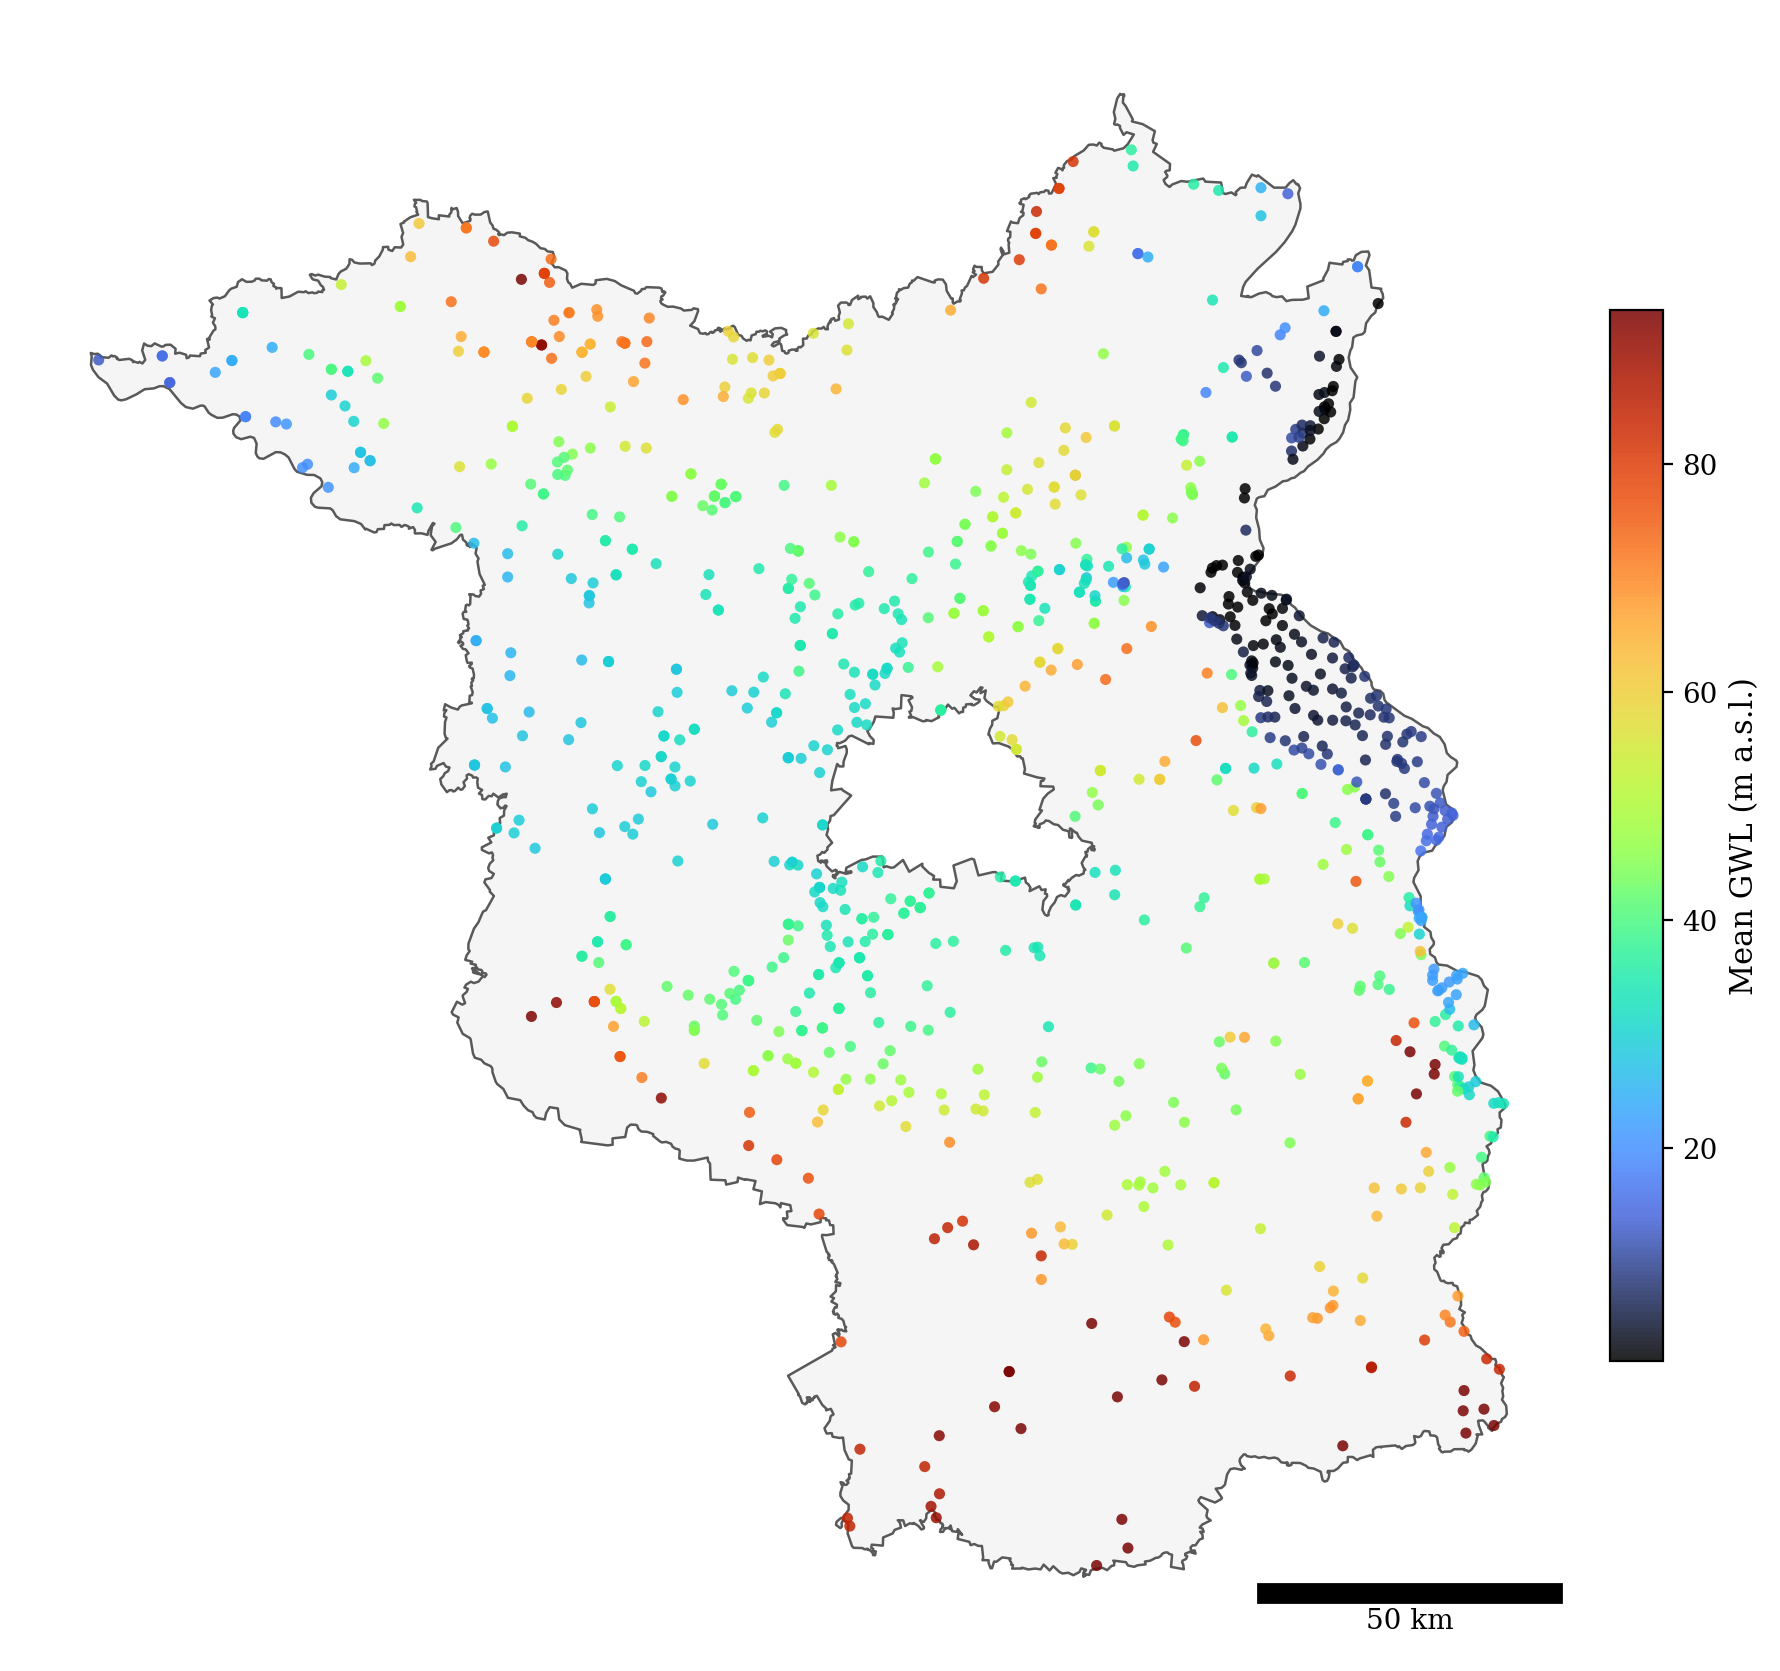
\includegraphics[width=0.85\textwidth]{mean_gwl_map}
  \caption{Mean GWL per well (m a.s.l., averaged over 2008--2024) across all 1{,}040 monitoring
  wells in Brandenburg; the hole in the middle marks Berlin, which is not part of the state. The
  color scale is clipped at the 2nd and 98th percentiles (1.3\,m and 93.6\,m) to prevent extreme
  wells from compressing the color range; the actual range spans 0.3\,m to 130.3\,m.}
  \label{fig:mean_gwl_map}
\end{figure}

\Cref{fig:gwl_timeseries} shows observed GWL time series at three representative wells, one
from each hydrogeological zone (recharge, transit, discharge). Each well is shown over a
three-year window from the test period for direct comparison. Seasonal cycles are
visible in all three, but the amplitude and mean level differ across zones.

\begin{figure}[htbp]
  \centering
  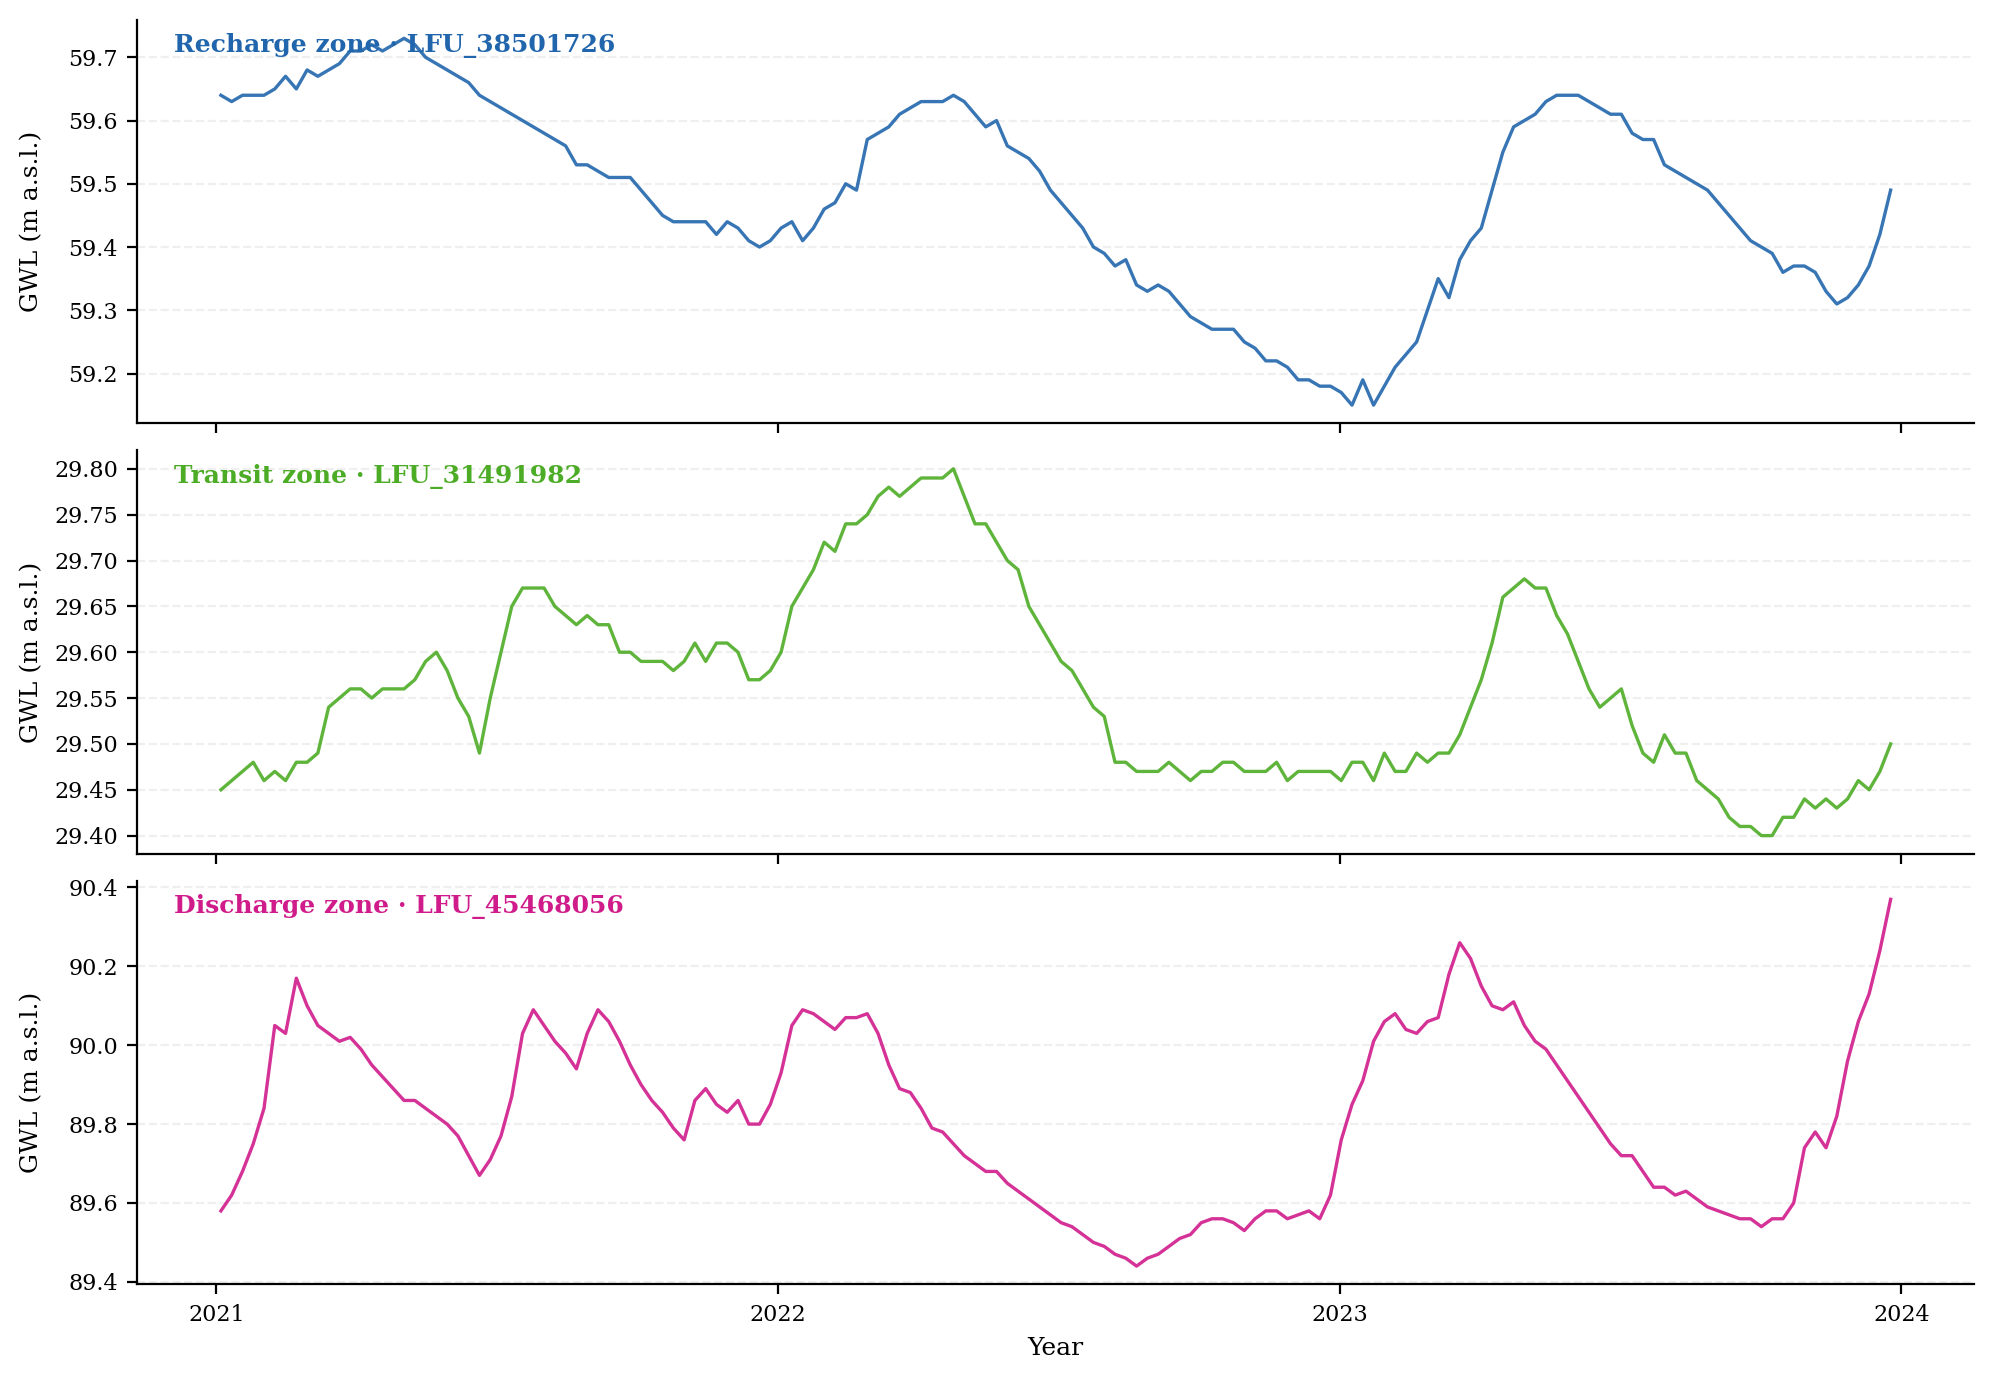
\includegraphics[width=\textwidth]{gwl_timeseries_hydroraum}
  \caption{GWL time series at three representative wells, one per hydrogeological zone}
  \label{fig:gwl_timeseries}
\end{figure}


\section{Features}
\label{sec:features}

Each well has dynamic meteorological features and static hydrogeological features.

\subsection{Dynamic Covariates}

Meteorological dynamic features are taken from HYRAS~5.0 \citep{razafimaharo2020}, a
gridded meteorological dataset produced by the German Weather Service (Deutscher
Wetterdienst, DWD). HYRAS~5.0 covers Germany with high-resolution meteorological grids. Daily
values are aggregated to weekly resolution. Meteorological values for each monitoring well are taken from the preprocessed dataset provided
by \citet{kunz2025}, aggregated within a 5\,km buffer as a weighted average across intersecting
grid pixels. The 5\,km resolution matches that of operational DWD weather forecasts, which allows
the pipeline to use forecast data in real-world deployment. The three HYRAS meteorological
variables together with two calendar encodings give five dynamic features in total. The
variables are:

\begin{enumerate}
  \item \textbf{Temperature} (°C) --- weekly mean of air temperature in 2\,m altitude
  \item \textbf{Relative humidity} (\%) --- weekly mean
  \item \textbf{Precipitation} (mm/week) --- accumulated weekly precipitation
  \item \textbf{Day-of-year (sine)} --- cyclic encoding $\sin(2\pi\,\text{DOY}/365.25)$
  \item \textbf{Day-of-year (cosine)} --- cyclic encoding $\cos(2\pi\,\text{DOY}/365.25)$
\end{enumerate}

The sine and cosine encoding lets the model pick up seasonal patterns and avoids jumps
when the year changes from December to January.

\subsection{Static Features}
\label{sec:static_features}

The dataset contains 40 static hydrogeological features per well, of which 35 are used as GRU inputs; 3 of those (the one-hot encoding of hydrogeological zone into recharge, transit, and discharge categories) are also used as GP spatial inputs. The remaining 5 features are available in the dataset but are not primary model inputs. Complete feature definitions, column names, and model assignments are in \cref{app:features}.

Three features are highlighted here because they appear prominently in the results.

\textbf{Hydrogeological zone} (\texttt{hydroraum}) classifies each well as sitting in a recharge zone (where rain infiltrates into the ground), a discharge zone (where groundwater flows out near streams), or a transit zone in between. Wells in different zones behave differently even under the same weather conditions (3 categories; 109, 528, and 403 wells respectively; \cref{fig:hydroraum_dist}). The GP feature ablation (\cref{sec:gp_ablation}) identifies this as the single most informative static covariate for spatial interpolation.

\textbf{Aquifer confinement} (\texttt{gw\_gespannt\_bin}) records whether the aquifer is confined or unconfined; 319 confined and 721 unconfined wells (\cref{fig:aquifer_dist}).

\textbf{Groundwater residence time} (\texttt{siwa\_verweilzeit\_j}) records how long water typically stays underground before surfacing again, in years (categories: 0, 1, 3, 10, 30, or 50; 43 wells with missing values; \cref{fig:siwa_dist}).

\begin{figure}[htbp]
  \centering
  \begin{minipage}[t]{0.47\textwidth}
    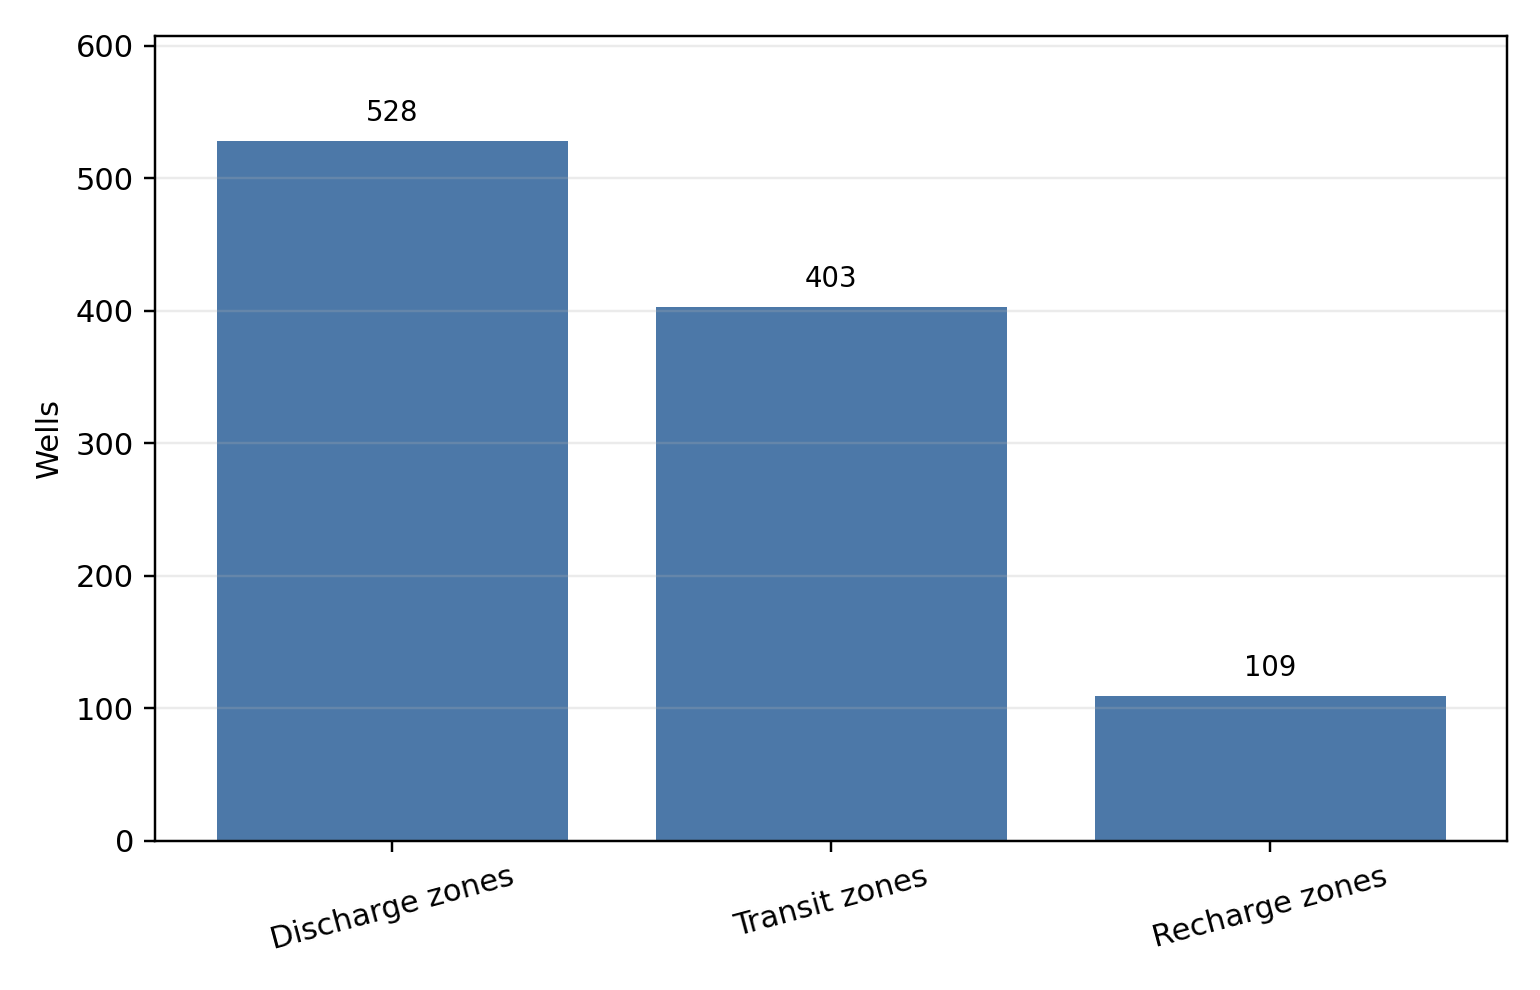
\includegraphics[width=\textwidth]{hydroraum_dist}
    \caption{Hydrogeological zone distribution across the 1{,}040 monitoring wells}
    \label{fig:hydroraum_dist}
  \end{minipage}
  \hfill
  \begin{minipage}[t]{0.47\textwidth}
    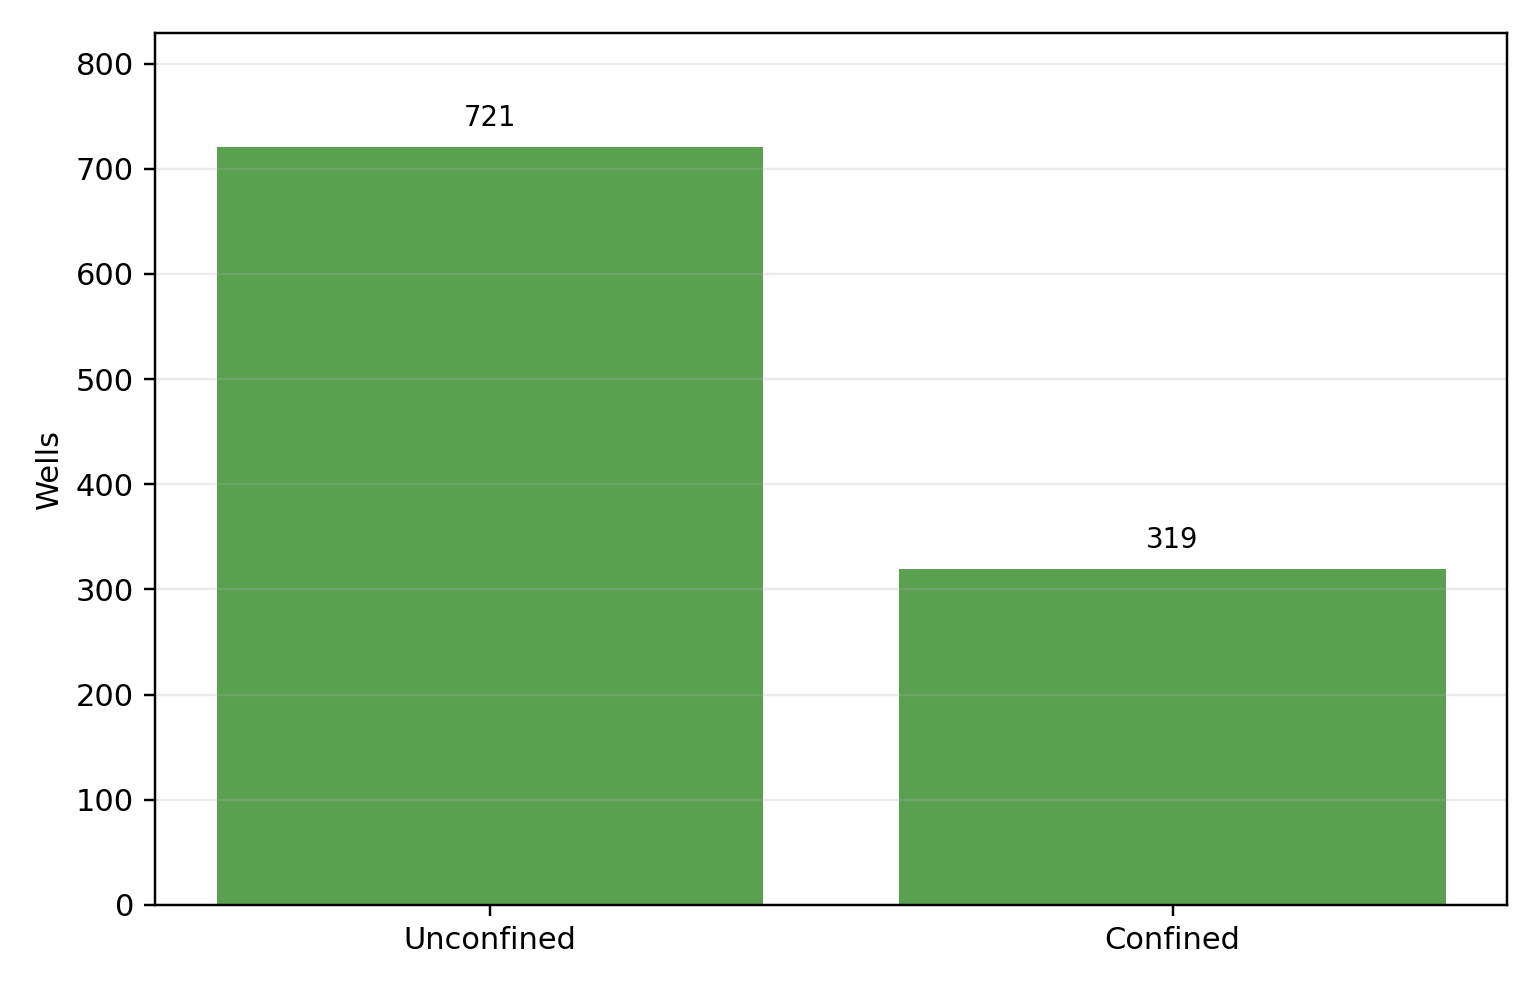
\includegraphics[width=\textwidth]{aquifer_dist}
    \caption{Aquifer confinement distribution across the 1{,}040 monitoring wells}
    \label{fig:aquifer_dist}
  \end{minipage}
\end{figure}

\begin{figure}[htbp]
  \centering
  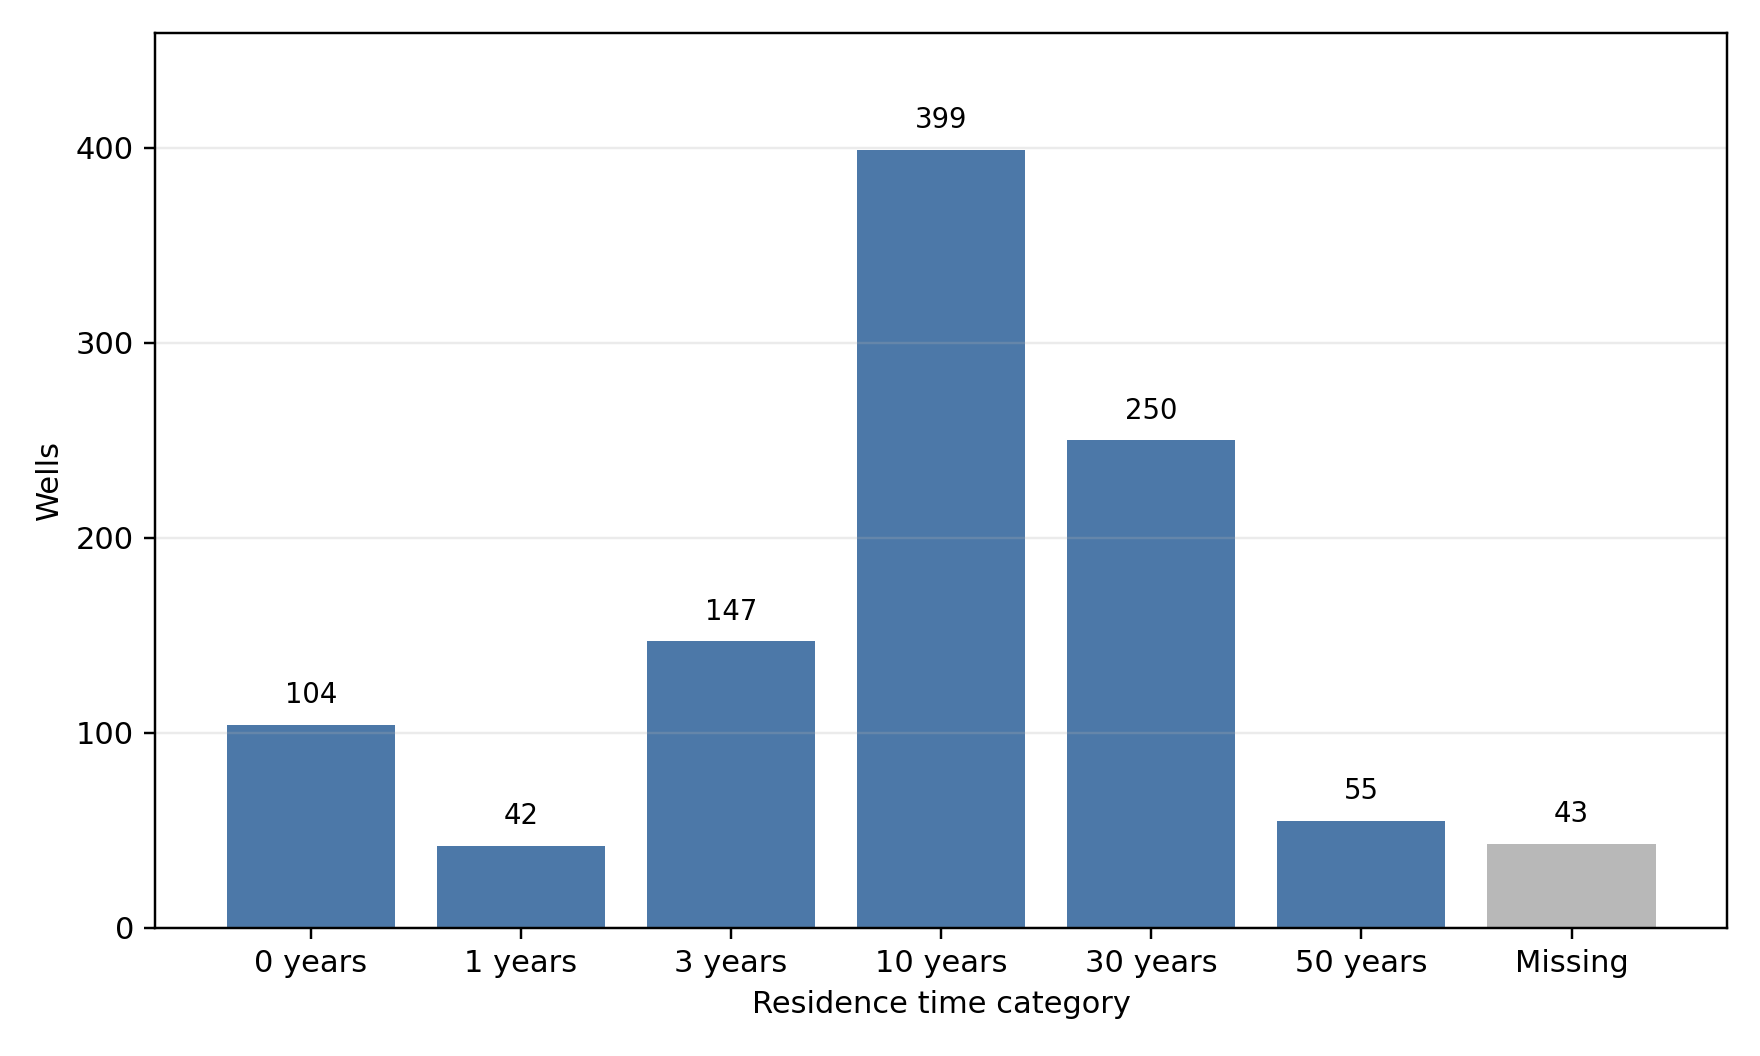
\includegraphics[width=0.65\textwidth]{siwa_dist}
  \caption{Groundwater residence time distribution}
  \label{fig:siwa_dist}
\end{figure}

\section{Data Preprocessing}
\label{sec:preprocessing}

The following preprocessing steps are applied, with steps 1--3 performed by \citet{kunz2025} and steps 4--5 applied in this work:

\begin{enumerate}
  \item \textbf{Temporal alignment:} All time series are resampled to ISO-week granularity
  (Monday-start weeks).
  \item \textbf{Gap imputation:} Gaps of up to 4 weeks are linearly interpolated; gaps of up to
  52 weeks are filled with a Bayesian imputer.
  \item \textbf{Well selection:} Only wells with consistent GWL time series starting no later
  than 2008 and having continuous values until 2024 (after the imputations in step\,2) are included.
  \item \textbf{GWL normalization:} GWL values are z-scored per well (zero mean and
  unit variance), using the mean and standard deviation computed on the training portion of
  each well's time series. This removes each well's individual long-term mean level, so the
  temporal model learns dynamics (deviations from the mean) rather than absolute levels. See
  \cref{sec:variation} for the motivation.
  \item \textbf{Feature normalization:} Continuous static and dynamic covariates (meteorological
  variables and static features) are standardized per feature, again using statistics computed 
  on the training set only.
\end{enumerate}

\subsection{Co-located Well Handling}
\label{sec:deduplication}

Several wells in the dataset share essentially
identical UTM coordinates (EPSG:25833) with at least one other well. This is the case at monitoring 
sites where multiple boreholes or screened intervals were installed at the same surface point, 
which is a common practice at sites requiring monitoring of different aquifer layers simultaneously.

This issue becomes clear during initial spatial evaluation experiments: the spatial GP
pipeline performs unusually well on certain test wells, in some cases even outperforming
the pure temporal GRU baseline that has been trained on past observations of those exact wells.
This is highly unexpected, since the GP interpolation to unmonitored locations should perform
substantially worse than a model trained directly on the well's own history. Further investigation
shows that these high-performing test wells have training-set neighbors at identical or
near-identical surface coordinates. Therefore, the GP effectively produces the prediction for
the unmonitored location by just copying the value of the co-located training well, not by
generalizing or interpolating spatially in any meaningful sense. This skews overall performance
metrics, since they are dominated (and unfairly improved) by those trivially easy cases rather
than by the model's ability to interpolate to genuinely unseen locations.

On the other hand, co-located boreholes can also hurt performance when their GWL values differ substantially. In that case, the GP still copies the value from the co-located training 
well (since the coordinates are identical), but the copied value can be a poor match for a well
in a completely different depth, which makes performance worse rather than better. Since there is 
no clean depth threshold that separates the cases where interpolation is too easy from the ones
where it is too hard, the cleanest solution is to put all co-located wells into the
training set. This makes sure all measurements are kept and we are not discarding valuable data.

More specifically, the split generation algorithm identifies all wells within 8\,m of at least
one other well (308 wells in total) and puts them permanently into the training set. These
wells are never eligible to appear in the test set.
This approach keeps all 1{,}040 wells in the dataset,
so no measurements are discarded, while guaranteeing that every well in the test set poses a genuine
spatial interpolation challenge. Preliminary experiments show that excluding wells by aquifer
type hurts performance, suggesting that having more training data matters more than having
perfectly clean data.

The remaining 732 wells make up the eligible test pool from which the random 90/10 split is drawn
(splitting all 1{,}040 wells randomly would not give meaningful results, because of the co-located wells).
This yields 104 test wells and 936 training wells per split seed.

% ============================================================
\section{Chapter Summary}
% ============================================================

This chapter describes the Brandenburg groundwater dataset: 1{,}040 wells with weekly GWL observations starting between 1951 and 2008 and ending in 2024, five dynamic meteorological features from HYRAS~5.0, and 40 static hydrogeological features per well (of which 35 are used as GRU inputs; see \cref{app:features}). The large ratio of spatial to temporal GWL variation (roughly 83:1 in median ranges) motivates the two-stage pipeline design (\cref{sec:design_overview}), and the 308 co-located wells are forced into training to prevent trivially easy test cases. The uneven spatial distribution of wells means test wells in different split seeds vary widely in their isolation from the nearest training neighbor. \Cref{ch:methods} presents the full methodological framework built on this dataset.
% Chapter 4 — Methods (Technical Background + System Design + Implementation)
% !TEX root = ../main.tex
% ============================================================
%  Chapter 4 — Methods
%  Merges: Technical Background (ex 02_background) +
%          System Design (ex 05_design) +
%          Implementation (ex 06_implementation)
% ============================================================

\chapter{Methods}
\label{ch:methods}

This chapter presents the full methodological framework in three parts.
\Cref{sec:background} provides the technical background on Gated Recurrent Units, Gaussian
Process regression, and the evaluation metrics used throughout.
\Cref{sec:system_design} describes the design of the temporal and spatial models, the pipeline variants, and the spatial split.
\Cref{sec:implementation} documents the software setup and compute infrastructure.

% ============================================================
\section{Technical Background}
\label{sec:background}
% ============================================================

% ------------------------------------------------------------
\subsection{Recurrent Neural Networks and the Gated Recurrent Unit}
\label{subsec:rnn_gru}
% ------------------------------------------------------------

\subsubsection{Sequence-to-Sequence Forecasting}

A sequence-to-sequence (seq2seq) model maps an input sequence of length $L$ to an output
sequence of length $H$. Given a window of $L$ historical observations and input features
$\mathbf{X} = (\mathbf{x}_1, \ldots, \mathbf{x}_L)$, the model predicts the next $H$ values
$\hat{\mathbf{y}} = (\hat{y}_{t+1}, \ldots, \hat{y}_{t+H})$. This study uses $L = 52$ weeks (one year of look-back) and $H = 16$ weeks (approximately four months of forecast horizon).

\subsubsection{Gated Recurrent Unit}

The Gated Recurrent Unit \citep{cho2014learning} is a recurrent neural network architecture
that addresses the vanishing gradient problem of standard RNNs through learnable gating
mechanisms. Given input $\mathbf{x}_t$ and previous hidden state $\mathbf{h}_{t-1}$, the GRU
computes:

\begin{align}
  \mathbf{z}_t &= \sigma\!\left(\mathbf{W}_z \mathbf{x}_t + \mathbf{U}_z \mathbf{h}_{t-1} + \mathbf{b}_z\right) \label{eq:gru_update}\\
  \mathbf{r}_t &= \sigma\!\left(\mathbf{W}_r \mathbf{x}_t + \mathbf{U}_r \mathbf{h}_{t-1} + \mathbf{b}_r\right) \label{eq:gru_reset}\\
  \tilde{\mathbf{h}}_t &= \tanh\!\left(\mathbf{W}_h \mathbf{x}_t + \mathbf{U}_h (\mathbf{r}_t \odot \mathbf{h}_{t-1}) + \mathbf{b}_h\right) \label{eq:gru_candidate}\\
  \mathbf{h}_t &= (1 - \mathbf{z}_t) \odot \mathbf{h}_{t-1} + \mathbf{z}_t \odot \tilde{\mathbf{h}}_t \label{eq:gru_hidden}
\end{align}

where $\sigma$ is the sigmoid function, $\odot$ stands for element-wise multiplication,
$\mathbf{z}_t$ is the update gate, $\mathbf{r}_t$ is the reset gate, $\tilde{\mathbf{h}}_t$
is the candidate new hidden state, $\mathbf{W}_z, \mathbf{W}_r, \mathbf{W}_h$ are learned input
weight matrices, $\mathbf{U}_z, \mathbf{U}_r, \mathbf{U}_h$ are learned hidden weight
matrices, and $\mathbf{b}_z, \mathbf{b}_r, \mathbf{b}_h$ are bias vectors. The update gate
controls how much of the previous hidden state is retained; the reset gate controls how much
of the past is forgotten when computing the candidate hidden state.

\subsubsection{Static Feature Integration}

Well-specific static features (hydrogeological covariates that are constant over time) are
integrated here by projecting them into the initial hidden state $\mathbf{h}_0$ via a learned
linear layer:

\begin{equation}
  \mathbf{h}_0^{(\ell)} = \mathbf{W}_s^{(\ell)} \mathbf{s} + \mathbf{b}_s^{(\ell)}, \quad \ell = 1, \ldots, L_\text{layers}
  \label{eq:static_init}
\end{equation}

where $\mathbf{s} \in \mathbb{R}^{d_s}$ is the static feature vector of dimension $d_s$,
$\mathbf{W}_s^{(\ell)}$ and $\mathbf{b}_s^{(\ell)}$ are the learned weight matrix and bias
for layer $\ell$, and $L_\text{layers}$ is the total number of GRU layers. This allows the
same model weights to be shared across all wells while the well-specific context is
encoded in the initial hidden state.

\subsubsection{Comparison to the Temporal Fusion Transformer}

The Temporal Fusion Transformer (TFT) \citep{lim2021temporal} is an attention-based seq2seq
architecture designed for multi-horizon forecasting with heterogeneous inputs. It incorporates
variable selection networks, gating mechanisms, and multi-head attention over the entire input
sequence. While TFT achieves strong performance on such tasks, it carries significantly more
parameters and longer training times than a GRU. The GRU is therefore selected as the
temporal model; a replication of the \citet{kunz2025} TFT baseline and a direct
performance comparison are presented in \cref{sec:gru_results}.
The GRU in this thesis is trained with MSE loss, which is standard for GRU regression models. RMSE is used as the evaluation metric for both models, so their values are directly comparable regardless of training loss.

% ------------------------------------------------------------
\subsection{Gaussian Process Regression}
\label{subsec:gp_background}
% ------------------------------------------------------------

\subsubsection{Definition}

A Gaussian Process is a distribution over functions $f: \mathcal{X}
\to \mathbb{R}$ such that any finite collection of function values is jointly Gaussian \citep{rasmussen2006gaussian}:

\begin{equation}
  f(\mathbf{x}_1), \ldots, f(\mathbf{x}_n) \sim \mathcal{N}\!\left(\boldsymbol{\mu}, \mathbf{K}\right)
\end{equation}

where $\mathbf{x}_i \in \mathcal{X}$ is the input point of the $i$-th well, $\boldsymbol{\mu}$ is the mean vector with $\mu_i = m(\mathbf{x}_i)$, and $\mathbf{K}$ is
the covariance matrix with $K_{ij} = k(\mathbf{x}_i, \mathbf{x}_j)$. The mean function $m(\cdot)$ and kernel $k(\cdot, \cdot)$ define what the GP assumes about
the function before seeing any data.

\subsubsection{Posterior Prediction}

Given training observations $\mathbf{y} = f(\mathbf{X}) + \boldsymbol{\varepsilon}$ with
$\boldsymbol{\varepsilon} \sim \mathcal{N}(\mathbf{0}, \sigma_n^2 \mathbf{I})$, the GP
posterior at test points $\mathbf{X}_*$ is:

\begin{align}
  \mathbf{f}_* \mid \mathbf{X}, \mathbf{y}, \mathbf{X}_* &\sim \mathcal{N}\!\left(\boldsymbol{\mu}_*, \boldsymbol{\Sigma}_*\right)\\
  \boldsymbol{\mu}_* &= m(\mathbf{X}_*) + \mathbf{K}_{*}\left(\mathbf{K} + \sigma_n^2 \mathbf{I}\right)^{-1}(\mathbf{y} - m(\mathbf{X}))\\
  \boldsymbol{\Sigma}_* &= \mathbf{K}_{**} - \mathbf{K}_{*}\left(\mathbf{K} + \sigma_n^2 \mathbf{I}\right)^{-1}\mathbf{K}_{*}^\top
\end{align}

where $\mathbf{K} = k(\mathbf{X}, \mathbf{X})$ is the training kernel matrix,
$\mathbf{K}_{*} = k(\mathbf{X}_*, \mathbf{X})$ is the cross-covariance between test and
training points, and $\mathbf{K}_{**} = k(\mathbf{X}_*, \mathbf{X}_*)$ is the test kernel
matrix, and $\sigma_n^2$ is the observation noise variance. The posterior mean $\boldsymbol{\mu}_*$ provides point predictions, while the
diagonal of $\boldsymbol{\Sigma}_*$ provides predictive variances.

\subsubsection{The Matérn-3/2 Kernel}

Matérn kernels control the smoothness of the modelled function. The Matérn-3/2 kernel is:

\begin{equation}
  k_{\text{M32}}(r) = \sigma^2 \left(1 + \frac{\sqrt{3}\,r}{\ell}\right) \exp\!\left(-\frac{\sqrt{3}\,r}{\ell}\right)
  \label{eq:matern32}
\end{equation}

where $r = \|\mathbf{x} - \mathbf{x}'\|$ is the Euclidean distance between two wells, $\ell$ is the length-scale (controlling how quickly spatial similarity decays with distance), and $\sigma^2$ is the output-scale (the overall variance of the GP). Matérn-3/2 assumes once-differentiable sample paths, meaning each function the GP contains has exactly one continuous derivative, which is a standard prior for spatially smooth but not infinitely smooth physical fields such as GWL.

\subsubsection{Kernel Hyperparameter Optimisation}

The kernel hyperparameters, length-scales $\boldsymbol{\ell}$, output scale $\sigma^2$, and noise variance $\sigma_n^2$, are not set by hand but learned from data by maximising the marginal log-likelihood (MLL). The MLL is the log probability of the observed targets $\mathbf{y}$ under the GP model, integrated over all possible latent function values. It balances data fit against model complexity, and its gradient with respect to the hyperparameters is available in closed form \citep{rasmussen2006gaussian}, which allows gradient-based optimisation.

\subsubsection{Exact Inference with GPyTorch}

Exact GP inference requires inverting the $n \times n$ kernel matrix, where $n$ is the
number of training points, which has $\mathcal{O}(n^3)$ time complexity and $\mathcal{O}(n^2)$ memory
complexity \citep{rasmussen2006gaussian}. Since there are at most 936 training wells per date in our setup, exact inference is computationally feasible. This thesis uses the GPyTorch library \citep{gardner2018gpytorch}
for its kernel and likelihood implementations, but solves the GP equations exactly using
Cholesky decomposition instead of GPyTorch's built-in approximate solvers, because $n \leq 936$ makes exact inference feasible and Cholesky gives the exact solution with no approximation error. Rather than computing $(\mathbf{K} + \sigma_n^2 \mathbf{I})^{-1}$ directly, Cholesky factorises $\mathbf{K} + \sigma_n^2 \mathbf{I} = \mathbf{L}\mathbf{L}^\top$, where $\mathbf{L}$ is a lower-triangular matrix. The posterior mean and variance then follow from two triangular solves rather than an explicit inversion, which is faster and numerically more stable. At $n \approx 936$, the Cholesky factorization involves roughly $10^8$ floating-point operations per fit, which completes in milliseconds on the GPU hardware used (see \cref{sec:compute}).

% ------------------------------------------------------------
\subsection{Evaluation Metrics}
\label{subsec:metrics}
% ------------------------------------------------------------

Results are reported primarily at forecast horizon $h = 16$ (16 weeks ahead), which is the most demanding horizon and therefore the most informative single value to report. The choice also allows comparability with unpublished experiments on the Brandenburg dataset shared by \citeauthor{kunz2025}; their published paper uses $h = 12$, but on a different dataset, so those published values are not directly comparable regardless. The mean of each metric over all 16 horizons is additionally reported. Each per-well value at a given horizon is averaged over all evaluation time steps $T_i$; distribution statistics are then computed across test wells.

\subsubsection{Root Mean Squared Error}

The per-well RMSE at forecast horizon $h$ is:

\begin{equation}
  \text{RMSE}_i^h = \sqrt{\frac{1}{|T_i|} \sum_{t} \left(\hat{y}_{i,t+h} - y_{i,t+h}\right)^2}
  \label{eq:rmse}
\end{equation}

where $i$ indexes the test well, $t$ indexes the evaluation time steps in $T_i$, $\hat{y}_{i,t+h}$ is the model prediction, and $y_{i,t+h}$ is the observed GWL value. The primary metric is $\text{RMSE}_i^{16}$; the mean $\overline{\text{RMSE}}_i = \frac{1}{H}\sum_{h=1}^{H} \text{RMSE}_i^h$ is additionally reported.

The following distributional summaries are reported to characterize both central tendency and
tail behavior: the mean $\pm$ standard deviation across test wells, and the percentiles
P10, P25, median (P50), P75, and P90 of the per-well RMSE distribution (\cref{tab:cross_split_full_metrics}). P10 marks the best-performing 10\% of wells; P90 is the threshold above which only the worst-performing 10\% fall; P25--P75 (interquartile range) shows how concentrated results are around the median.

\subsubsection{Normalized RMSE per Well (nRMSE\textsubscript{pw})}

Because GWL ranges vary across wells, raw RMSE is larger for wells with bigger amplitudes even at equal model accuracy; normalizing by a well-specific scale removes this and gives each well equal weight:

\begin{equation}
  \text{nRMSE}^\text{IQR}_{\text{pw},i} = \frac{\text{RMSE}_i}{\text{IQR}(y_{i,\cdot})}
  \label{eq:nrmse_iqr}
\end{equation}

where $\text{IQR}(y_{i,\cdot}) = Q_{75}(y_{i,\cdot}) - Q_{25}(y_{i,\cdot})$ is the interquartile range of observed GWL values at well $i$. The result is aggregated as the median across test wells. Range normalization, $\text{RMSE}_i / \text{range}(y_{i,\cdot})$ where $\text{range}(y_{i,\cdot}) = \max(y_{i,\cdot}) - \min(y_{i,\cdot})$, is a natural alternative, but across the wells in this study the range is about $3$--$4\times$ larger than the IQR and more sensitive to extreme observations. IQR normalization is therefore more robust and is the single reported normalized metric. It is used for pipeline comparison and for the GP feature ablation (\cref{sec:gp_ablation}).

\subsubsection{Nash--Sutcliffe Efficiency}

The Nash--Sutcliffe Efficiency (NSE) \citep{nash1970river} measures the fraction of variance
explained relative to a climatological mean baseline:

\begin{equation}
  \text{NSE}_i^h = 1 - \frac{\sum_t (\hat{y}_{i,t+h} - y_{i,t+h})^2}{\sum_t (\bar{y}_i - y_{i,t+h})^2}
  \label{eq:nse}
\end{equation}

where $i$, $t$, $h$, $\hat{y}_{i,t+h}$, $y_{i,t+h}$ are as in \cref{eq:rmse}, and $\bar{y}_i$ is the per-well mean GWL baseline. Two choices exist
for $\bar{y}$: the test-period mean or the training-period mean.
This study uses the test-period mean as the primary choice, consistent with the original
formulation of \citet{nash1970river}, who define $\bar{y}$ as the mean of observed values
over the evaluation period, the standard in hydrology.
The primary metric is $\text{NSE}_i^{16}$; the mean $\overline{\text{NSE}}_i = \frac{1}{H}\sum_{h=1}^{H} \text{NSE}_i^h$ is additionally reported. NSE $\in (-\infty, 1]$: a value of 1 indicates perfect prediction, 0 indicates no better than the mean, and negative values indicate worse-than-mean performance.

NSE is reported for all models. For the temporal models it is a standard performance measure; for the spatiotemporal pipeline, the structural disadvantage means values will be strongly negative and should be interpreted accordingly. For spatial test wells, NSE has a structural disadvantage compared to the temporal models: its baseline uses the per-well mean $\bar{y}$, which is
derived from observations at that specific well, which is information the GP never has access to
during training. Both the temporal models and the GP use the per-well test-period mean as the NSE baseline, which neither model has seen during training. The disadvantage is larger for spatial interpolation, though: the GP has to estimate GWL levels per timestep at unobserved wells across a range of roughly 130\,m, while each temporal model works within a single well whose amplitude over the entire time span is on average around 1.5\,m and has a maximum value of 16\,m. Missing the absolute level by even a small fraction of the range produces a much larger NSE penalty than a comparable relative miss within a single well.
As a result, spatiotemporal pipeline NSE values are strongly negative, regardless of pipeline variant (mean $\approx -38.4$ for the primary 90/10 evaluation) and are reported in the results.

\subsubsection{Kling-Gupta Efficiency}
\label{subsec:kge}

The Kling-Gupta Efficiency \citep{gupta2009decomposition} separates prediction error into
three components (correlation, variability, and bias), which gives a more complete picture
than NSE alone:

\begin{equation}
  \text{KGE} = 1 - \sqrt{(r-1)^2 + (\alpha-1)^2 + (\beta-1)^2}
  \label{eq:kge}
\end{equation}

where $r$ is the Pearson correlation coefficient between predicted and observed values,
$\alpha = \sigma_s / \sigma_o$ is the ratio of simulated to observed standard deviation
(variability ratio), and $\beta = \mu_s / \mu_o$ is the ratio of simulated to observed mean
(bias ratio). A perfect model achieves KGE $= 1$; values closer to 1 are better. Unlike NSE, always predicting the observed mean does not correspond to KGE $= 0$:
it typically gives KGE $\approx -0.41$ \citep{knoben2019intercomparison}, so KGE $= 0$ already represents a model that
outperforms that baseline. Unlike NSE, which is based on squared residuals alone, KGE explicitly accounts for correlation, variability, and bias in how it penalizes prediction errors.
Per-well KGE is computed using the same predicted and observed values as RMSE and NSE.

\subsubsection{Global (Pooled) Metrics}
\label{subsec:global_metrics}

Per-well summary statistics treat each well as an independent observation and are robust to
outliers. Complementarily, global metrics pool all errors across all test wells
$i \in \mathcal{W}_\text{test}$, all evaluation time steps $t$, and all horizons $h$:

\begin{align}
  \text{RMSE}_\text{global} &= \sqrt{\frac{1}{|\mathcal{W}_\text{test}| \cdot |T| \cdot H}
    \sum_{i,t,h} \left(\hat{y}_{i,t+h} - y_{i,t+h}\right)^2}
  \label{eq:global_rmse}\\
  \text{NSE}_\text{global} &= 1 - \frac{\sum_{i,t,h} (\hat{y}_{i,t+h} - y_{i,t+h})^2}
    {\sum_{i,t,h} (\bar{y} - y_{i,t+h})^2}
  \label{eq:global_nse}
\end{align}

where $\mathcal{W}_\text{test}$ is the set of test wells, $|T|$ is the number of evaluation
time steps, $H = 16$ is the forecast horizon length, $\bar{y}$ is the global mean over all
pooled observations, and $i$, $t$, $h$, $\hat{y}_{i,t+h}$, $y_{i,t+h}$ are as defined in
\cref{eq:rmse}. Global RMSE gives more weight to the worst-performing wells (squaring errors amplifies large deviations, so a few badly-predicted wells raise it noticeably), so it picks up issues the per-well median can miss. Global NSE uses the grand mean across all pooled observations as its baseline, so a model that predicts the grand mean everywhere scores 0. A model only needs to place each well's mean on the correct side of the grand mean to beat this baseline; with a range of roughly 130\,m across Brandenburg wells, that is not a hard task. The GP does exactly this, since spatial interpolation of between-well level differences is its core task. Per-well NSE uses each well's own test-period mean as the baseline. The temporal range within a single well averages roughly 1.5\,m, so the per-well mean is at most about 0.75\,m from any observation in an average well. To score above zero on per-well NSE, the GP would have to predict each well's absolute GWL to within that margin, on a scale that spans 130\,m across the study area, which is not achievable for a model that has never observed that well. The result is global NSE around $+0.92$ and per-well NSE around $-33$ for the spatiotemporal pipeline, and both are reported in the results.

\subsubsection{Prediction Interval Coverage Probability}

The GP spatial interpolation stage outputs a predicted GWL $\hat{y}_t$ and a posterior standard deviation $\hat{\sigma}_t$ at each test well. A $(1-\alpha)$ prediction interval is $[\hat{y}_t - z_{\alpha/2}\hat{\sigma}_t,\; \hat{y}_t + z_{\alpha/2}\hat{\sigma}_t]$, where $\alpha$ is the tail probability and $z_{\alpha/2}$ is the standard normal quantile; for a 90\% interval, $\alpha = 0.10$ and $z_{0.05} \approx 1.645$. PICP measures the fraction of true observations that fall inside:

\begin{equation}
  \text{PICP} = \frac{1}{N}\sum_{i=1}^{N} \mathbf{1}\!\left[y_i \in [\hat{y}_i - z_{\alpha/2}\hat{\sigma}_i,\; \hat{y}_i + z_{\alpha/2}\hat{\sigma}_i]\right]
\end{equation}

A well-calibrated model achieves $\text{PICP} \approx 1-\alpha$: for a 90\% interval, roughly 90\% of observations should fall inside. If coverage is too low the model is overconfident; if too high, the intervals are unnecessarily wide.

\subsubsection{Statistical Tests}
\label{sec:statistical_tests}

Two statistical tests are used to quantify the strength and significance of relationships in the multi-seed evaluation.

The \textbf{Spearman rank correlation} $\rho$ measures the monotonic association between two variables without assuming a linear relationship or normal distribution. It is computed on ranks rather than raw values, making it robust to outliers. A value of $\rho = 1$ indicates a perfect positive monotonic relationship; $\rho = 0$ indicates no monotonic association. The associated $p$-value tests the null hypothesis that the two variables are uncorrelated in the population.

The \textbf{paired $t$-test} compares the means of two matched samples. In this thesis it is applied to the per-seed difference in RMSE between two pipeline configurations evaluated on the same 40 random splits. The test statistic is $t = \bar{d} / (s_d / \sqrt{n})$, where $\bar{d}$ is the mean pairwise difference, $s_d$ its standard deviation, and $n = 40$ the number of split seeds. The two-sided $p$-value tests the null hypothesis that the true mean difference is zero.

% ------------------------------------------------------------
\subsection{Hyperparameter Optimization}
\label{subsec:hpo}
% ------------------------------------------------------------

Hyperparameters for both the GRU and the GP are selected by iterative grid search over
predefined search spaces. Each round evaluates all combinations in the grid, identifies the
best-performing configuration, and uses it to define a narrower search space for the next
round. Four rounds are run for the GRU and three for the GP. GRU configurations are
evaluated on a temporal validation set (2016--2019); GP configurations are
evaluated on spatial validation wells.

% ============================================================
\section{System Design}
\label{sec:system_design}
% ============================================================

% ------------------------------------------------------------
\subsection{Overview}
\label{sec:design_overview}
% ------------------------------------------------------------

The GIST system addresses two coupled prediction tasks: temporal forecasting and spatial
interpolation. The high-level design decomposes the problem into two stages, which can be
executed independently (two-stage spatiotemporal pipeline) or trained jointly (jointly trained spatiotemporal model). A third
configuration replaces GRU outputs with true observations to isolate the contribution of
each stage (true-observation interpolation baseline).

The large spatial-to-temporal variance ratio in the dataset (\cref{sec:variation}) means a model needs to separate the long-term mean level at each location from the temporal dynamics. Per-well normalization handles this by subtracting each well's long-term mean level and dividing by its standard deviation before training, so the model learns deviations rather than absolute groundwater levels. This decomposition into a spatial per-well mean and temporal deviations motivates the two-stage pipeline: the GRU learns temporal dynamics on normalized series, after which the GP reconstructs the spatial mean at unobserved locations. \citet{kunz2025} apply no per-well normalization; as a result, the standard deviation of GWL is their single most important static feature.

Beyond predictive accuracy, the evaluation includes explicit interpretability analyses. A GRU feature permutation importance study and a systematic GP feature ablation, both in \cref{ch:results}, show which input features the GRU relies on for temporal forecasting and which spatial features the GP relies on for interpolation.

\Cref{fig:pipeline_overview} shows the three model configurations. In all cases, the
final output is a 16-week GWL forecast for each of the test wells.

\begin{figure}[htbp]
  \centering
  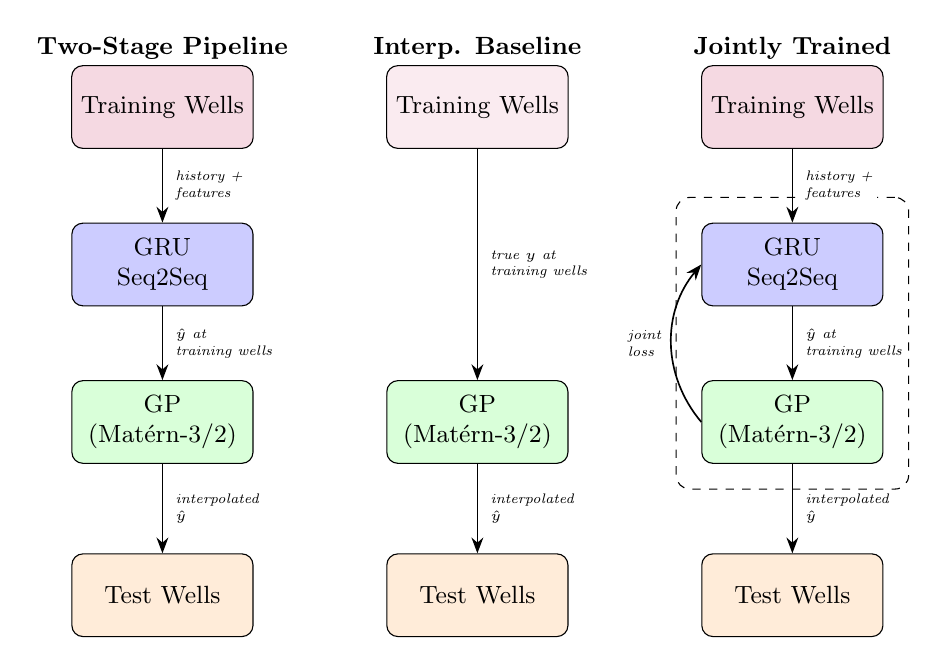
\begin{tikzpicture}[
    box/.style={rectangle, draw, rounded corners=4pt,
                minimum height=1.05cm, minimum width=2.3cm,
                align=center, font=\small},
    arrow/.style={-Stealth, semithick},
    lbl/.style={font=\tiny\itshape, fill=white, inner sep=1.5pt, align=left},
    head/.style={font=\small\bfseries, align=center},
  ]

  % Column x-centres and row y-centres (absolute positioning)
  % Three pipelines flow top-to-bottom in side-by-side columns.
  % Levels: 1=input  2=GRU  3=GP  4=output
  % True-Observation Baseline skips level 2; the longer arrow signals the absent temporal model.

  \def\xA{1.5}   % Two-Stage column
  \def\xB{5.5}   % True-Observation Baseline column
  \def\xC{9.5}   % Jointly Trained column

  \def\yTitle{0.55}
  \def\yOne{-0.2}    % input box
  \def\yTwo{-2.2}    % GRU box
  \def\yThree{-4.2}  % GP box
  \def\yFour{-6.4}   % output box

  % ── Two-Stage Pipeline ──────────────────────────────────────────────
  \node[head] at (\xA cm, \yTitle cm) {Two-Stage Pipeline};

  \node[box, fill=purple!15]  (dI) at (\xA cm, \yOne cm)   {Training Wells};
  \node[box, fill=blue!20]   (dG) at (\xA cm, \yTwo cm)   {GRU\\Seq2Seq};
  \node[box, fill=green!15]  (dP) at (\xA cm, \yThree cm) {GP\\(Mat\'{e}rn-3/2)};
  \node[box, fill=orange!15] (dO) at (\xA cm, \yFour cm)  {Test Wells};

  \draw[arrow] (dI.south) -- (dG.north)
    node[midway, right=3pt, lbl] {history +\\features};
  \draw[arrow] (dG.south) -- (dP.north)
    node[midway, right=3pt, lbl] {$\hat{y}$ at\\training wells};
  \draw[arrow] (dP.south) -- (dO.north)
    node[midway, right=3pt, lbl] {interpolated\\$\hat{y}$};

  % ── True-Observation Interpolation Baseline ──────────────────────────
  \node[head] at (\xB cm, \yTitle cm) {Interp. Baseline};

  \node[box, fill=purple!8]   (oI) at (\xB cm, \yOne cm)   {Training Wells};
  \node[box, fill=green!15]  (oP) at (\xB cm, \yThree cm) {GP\\(Mat\'{e}rn-3/2)};
  \node[box, fill=orange!15] (oO) at (\xB cm, \yFour cm)  {Test Wells};

  % Long arrow (spans level 2 gap) – signals absence of temporal model
  \draw[arrow] (oI.south) -- (oP.north)
    node[midway, right=3pt, lbl] {true $y$ at\\training wells};
  \draw[arrow] (oP.south) -- (oO.north)
    node[midway, right=3pt, lbl] {interpolated\\$\hat{y}$};

  % ── Jointly Trained Spatiotemporal Model ─────────────────────────────
  \node[head] at (\xC cm, \yTitle cm) {Jointly Trained};

  \node[box, fill=purple!15]  (jI) at (\xC cm, \yOne cm)   {Training Wells};
  \node[box, fill=blue!20]   (jG) at (\xC cm, \yTwo cm)   {GRU\\Seq2Seq};
  \node[box, fill=green!15]  (jP) at (\xC cm, \yThree cm) {GP\\(Mat\'{e}rn-3/2)};
  \node[box, fill=orange!15] (jO) at (\xC cm, \yFour cm)  {Test Wells};

  \node[draw, dashed, rounded corners=5pt, inner sep=0.32cm,
        fit=(jG)(jP)] (jbox) {};

  \draw[arrow] (jI.south) -- (jG.north)
    node[midway, right=3pt, lbl] {history +\\features};
  \draw[arrow] (jG.south) -- (jP.north)
    node[midway, right=3pt, lbl] {$\hat{y}$ at\\training wells};
  \draw[arrow] (jP.south) -- (jO.north)
    node[midway, right=3pt, lbl] {interpolated\\$\hat{y}$};
  \draw[arrow] (jP.west) to[bend left=40]
    node[pos=0.5, left=2pt, lbl] {joint\\loss} (jG.west);

  \end{tikzpicture}
  \caption{The three model configurations evaluated in this thesis ($y$: true observed GWL; $\hat{y}$: model prediction). In the two-stage spatiotemporal pipeline (left), the GRU and GP are trained independently: the GRU forecasts GWL at training wells, and the GP spatially interpolates those forecasts to test wells. The true-observation interpolation baseline (centre) replaces GRU forecasts with true observations, giving an upper bound on what the two-stage pipeline can achieve if the temporal forecasts are perfect. In the jointly trained spatiotemporal model (right), GRU and GP are trained end-to-end with a joint loss.}
  \label{fig:pipeline_overview}
\end{figure}

% ------------------------------------------------------------
\subsection{Temporal Split}
\label{sec:temporal_split}
% ------------------------------------------------------------

All 1{,}040 wells are assigned to one of three temporal periods. The
\textbf{training period} covers each well's available data from its start of coverage
(between 1951 and 2008) through the end of 2015 and is the only period on which GRU weights
are updated. The \textbf{validation period} covers 2016 through the end of 2019 and is used
for GRU hyperparameter optimisation and early stopping. The \textbf{test period} covers 2020
through mid-2024 and is held out until final evaluation. All spatiotemporal forecasts reported
in this thesis are evaluated on test-period predictions at spatial test wells that are never
seen during training.

% ------------------------------------------------------------
\subsection{Spatial Test Split}
\label{sec:spatial_splits}
% ------------------------------------------------------------

\subsubsection{Co-location Constraint}
\label{sec:coloc_constraint}

Before the split is drawn, all wells within 8\,m of at least one other well are permanently assigned to training (see \cref{sec:deduplication}). This leaves 732 eligible test wells.

\subsubsection{Random Split}

Wells are randomly assigned to train and test sets. The primary
evaluation uses a 90/10 split on the full 1{,}040-well dataset under the co-location constraint,
giving 936 training wells and 104 test wells with independent randomisation across 40
different split seeds. In a random split, test wells are distributed geographically among training wells (\cref{fig:random_split}).

Brandenburg has an unusually dense groundwater monitoring network (see \cref{sec:dataset}). The core question of this thesis is what such a network can achieve for the forecast-anywhere problem.
An 80\% training fraction is not used: test-set stability is already sufficient at 104 wells per seed, and the larger training set at 90\% better reflects what Brandenburg's full monitoring network can achieve, which is the core question of this study.
A 95\% training fraction is also tested but dropped: with only about 52 test wells per seed, per-seed RMSE is noisy and the across-seed standard deviation is high.
The 90/10 split keeps 936 training wells close to the full available network while giving 104 test wells per seed for stable aggregate statistics.
The 10\% final test fraction is also consistent with \citet{kunz2025}, who reserve similar fractions for temporal validation and test.

\begin{figure}[H]
  \centering
  
\includegraphics[width=0.72\textwidth]{spatial_split_rand90_ss42_presentation}
  \caption{Random 90/10 spatial test split (blue = training, orange = test). Co-located wells are forced into training. Test wells are distributed geographically across the monitoring network.}
  \label{fig:random_split}
\end{figure}

\subsubsection{Why Leave-One-Out Cross-Validation Was Not Used}
\label{sec:loocv_rationale}

Leave-one-out cross-validation (LOOCV) is a natural candidate for spatial evaluation, but
it is not considered an appropriate protocol for the research question this thesis addresses.

\paragraph{Conceptual mismatch.}
As discussed in \cref{sec:rw_ungauged}, LOOCV retains each test well's closest spatial
neighbors in training, so the GP interpolates over a very short spatial gap and the measured
error reflects gap-filling within a near-complete network rather than generalization to
genuinely unmonitored locations. Co-located wells could in principle be included by grouping wells at the same location and holding out entire groups, but some test folds would then contain multiple test wells, which complicates the procedure.

Furthermore, the key empirical finding of this thesis (that per-well interpolation error
correlates positively with distance to the nearest training neighbor) would be essentially
invisible under LOOCV: by construction, most test wells have a very close training
neighbor, so the error distribution would be heavily concentrated near zero distance and miss
the tail behavior that is the most scientifically interesting part of the result.

\paragraph{Computational cost.}
For a global GRU model, LOOCV would require 732--1{,}039 separate full pipeline runs (depending on how co-located wells are handled), making this approach infeasible at this data scale: at roughly 24 minutes per two-stage pipeline run, that amounts to approximately 13--18 days of compute on a single GPU, and approximately 30--45 days for the jointly trained pipeline.

\subsubsection{Alternative Test Strategies}
\label{sec:alt_splits}

Three additional test configurations are explored alongside the primary random split to assess how the choice of split design shapes reported performance. All three are evaluated as a sensitivity analysis in \cref{sec:split_sensitivity}.

\paragraph{Dense-area split.}
All distances between each eligible (non-co-located) well and its three nearest neighbors are computed and ranked. The 50th percentile of this distribution identifies the wells with the shortest typical neighborhood distances, those in the denser half of the monitoring network. Test wells are then drawn randomly from this restricted pool at a 90/10 fraction. Because every test well in the Dense-area split is drawn from an area with close training neighbors, the spatial interpolation task is easier on average than under a fully random draw. The 50th percentile is a fixed design boundary, not a tuned threshold: lowering it would change which wells are in the training set, making it a different experiment rather than a sensitivity check on the same model.

\paragraph{Cluster-stratified split.}
The 732 eligible (non-co-located) wells are partitioned into $k = 20$ clusters using $k$-means on all 35 static hydrogeological features. A fixed fraction of approximately 14\% is drawn from each cluster, giving a total close to 98 test wells; the exact count may differ by a few wells due to rounding within clusters. This distributes test wells uniformly across the static-feature space, regardless of their spatial position. Unlike the random split, which distributes training and test wells geographically at random, this strategy ensures that every part of the hydrogeological feature space is represented in both training and test sets.

\paragraph{Sparse-area split.}
The Sparse-area split reverses the logic of the Dense-area split: test wells are drawn from the 20\% of eligible (non-co-located) wells with the largest nearest-neighbor distances among eligible wells, those above the 80th percentile of that distribution; every test well therefore lies in a sparse area of the monitoring network. This creates a harder interpolation task than the random split, since the GP must generalize over larger distances with fewer nearby training wells. The two area-based splits cover opposite ends of interpolation difficulty: the Dense-area split creates an easier interpolation task, the Sparse-area split a harder one.

The area-based splits are not equivalent to post-hoc subsampling: by reassigning wells between train and test, they change the data the model trains on, so the same model cannot be evaluated under both conditions without retraining. The cluster-stratified split additionally guarantees feature-space coverage that random sampling may not provide. The sensitivity analyses therefore test generalization under genuinely different training conditions, and their consistency with the random-split results strengthens rather than merely repeats that evidence.

% ------------------------------------------------------------
\subsection{GRU Model Design}
\label{sec:gru_design}
% ------------------------------------------------------------

The GRU follows the seq2seq architecture described in \cref{subsec:rnn_gru}.
It consists of six stages:
\begin{enumerate}[label=\textcircled{\small\arabic*}]
  \item \textit{Data preparation.} The 1\,040 wells are split spatially into train and test sets.
    The temporal axis is further divided into a training, validation, and test period on the spatial train wells.
    GWL is normalized per well (z-score); weather covariates and static features are normalized globally.
    A sliding-window procedure creates overlapping 52-week input / 16-week output samples, with a 1-week shift between consecutive windows.
  \item \textit{Model inputs.} Each sample contains \texttt{x\_past} (52 time steps of GWL and 5 weather covariates),
    \texttt{x\_future} (16 time steps of future weather covariates), \texttt{x\_static} (35 static well attributes),
    and \texttt{y\_future} (16 normalized GWL values used as training targets).
  \item \textit{Static projection.} The 35 static features are passed through a linear layer
    (\texttt{Linear(35 $\to$ 256\,$\times$\,4\,=\,1\,024)}) and reshaped to provide each of the 4 encoder layers
    with a dedicated 256-dimensional initial hidden state, encoding the identity and characteristics of the well.
  \item \textit{Encoder GRU.} The encoder has 4 layers with 256 nodes each and dropout 0.2 between layers.
    It processes the 52-week input sequence step by step; the final hidden state of each layer is passed to the corresponding decoder layer.
  \item \textit{Decoder GRU.} The decoder has the same 4-layer, 256-node structure.
    It is initialized with the encoder's final hidden state and processes 16 steps of future weather covariates as step-by-step input,
    autoregressively building up a representation of the forecast period.
  \item \textit{Output head, denormalization, and predictions.} A linear layer (\texttt{Linear(256 $\to$ 1)}) is applied
    to each of the 16 decoder outputs, producing 16 normalized GWL predictions.
    These are then denormalized using the per-well z-score parameters fitted on the training period,
    converting each value back to absolute GWL in metres above mean sea level.
    During training, the mean squared error between the normalized predictions and \texttt{y\_future} is used as the loss.
\end{enumerate}

\Cref{fig:twostage_pipeline} illustrates the complete architecture across all six stages.

\subsubsection{GRU Static Features}
\label{sec:gru_static_features}

The GRU uses 35 static features per well, drawn from the full feature set described in
\cref{sec:features}. The raw aquifer confinement flag is replaced by its binarized equivalent (\texttt{gw\_gespannt\_bin}), keeping the total at 35.
The hydrogeological zone is used both as a GRU input (one-hot encoded into three categories) and
as the primary GP spatial feature (\cref{sec:gp_design}), where the GP feature ablation
identifies it as the single most informative covariate for spatial interpolation
(\cref{sec:gp_ablation}).

\subsubsection{Best Hyperparameter Configuration}

The best GRU configuration is identified through iterative grid search (\cref{subsec:hpo}) over hidden dimension, layer count,
dropout, learning rate, and batch size, evaluated on a temporal validation period.
The selected configuration is:

\begin{itemize}
  \item \textit{Architecture:} hidden dimension 256, 4 layers, dropout 0.2
  \item \textit{Optimisation:} learning rate $2 \times 10^{-4}$, batch size 4096, up to 50 epochs with early stopping (patience~$= 5$)
  \item \textit{Sequence lengths:} input window 52 weeks, output horizon 16 weeks
\end{itemize}

This configuration trains in roughly 20 minutes on an NVIDIA A100 GPU and is used for
all multi-seed spatiotemporal forecast interpolation experiments throughout this thesis.

% ------------------------------------------------------------
\subsection{Gaussian Process Design}
\label{sec:gp_design}
% ------------------------------------------------------------

The GP interpolation pipeline takes GRU-predicted GWL values at all training wells, together
with their coordinates and hydrogeological zone (one-hot encoded), and assembles them per
forecast horizon. For each horizon separately, an exact Gaussian Process with a Matérn-3/2
kernel is fitted. The kernel uses Automatic Relevance Determination (ARD): each input feature
gets its own length-scale, so the model learns how much geographic distance and zone membership
matter for spatial similarity. The fitted GP produces a GWL prediction and an uncertainty
estimate at each test well.

\subsubsection{Input Space}

The GP operates on a per-timestep snapshot: at each forecast date and horizon, the vector of
GWL values at all training wells is treated as a spatial field. The input $\mathbf{x}_i$ to
the GP is the coordinate vector of well $i$, optionally augmented with
static hydrogeological features. GRU predictions
at training well locations serve as the target vector $\mathbf{y}$ in the GP equations
(\cref{subsec:gp_background}); in the true-observation interpolation baseline, true observations are used
instead. The GP posterior then yields predictions at test well locations.

\subsubsection{Mean Function}

A zero mean function is used. Preliminary multi-seed experiments show a constant mean function performs worse, likely because the kernel's output scale already captures the overall level and a constant offset adds nothing.

\subsubsection{Kernel}

The Matérn-3/2 kernel (\cref{eq:matern32}) is applied in the augmented input space
(coordinates + static features). Automatic Relevance Determination (ARD) is used: each input
dimension receives its own length-scale parameter $\ell_d$, allowing the kernel to weight
coordinate dimensions and static features differently. The ARD length-scales are jointly
optimized with the noise variance and output scale via marginal likelihood maximisation.

\subsubsection{Kernel Pretraining and Per-Date Inference}
\label{sec:gp_inference_procedure}

Evaluating the GP across all test dates and forecast horizons requires fitting kernel hyperparameters in a way that is computationally tractable and consistent. The procedure used here has two levels.

\textbf{Per-horizon kernel pretraining.} For each of the 16 forecast horizons separately, all available training-well predictions (or true observations, for the interpolation baseline) across the entire test period are pooled into a single dataset. From this pooled dataset, 128 points are randomly subsampled and used to optimize the Matérn-3/2 kernel hyperparameters (length-scales, output scale, and noise variance) by maximising the marginal log-likelihood via 300 steps of Adam gradient descent \citep{kingma2015adam}, an adaptive-moment optimizer that maintains per-parameter learning rates. This yields 16 sets of kernel hyperparameters, one per horizon (\cref{app:gp_hpo}). The pooled dataset spans the full test period and covers the full spatial distribution of training wells, so even a small subsample represents the global spatial correlation structure well; 128 points suffice for a 7-parameter kernel optimization, and the per-date Cholesky inference that follows uses all $n \approx 936$ training wells.

\textbf{Per-(date, horizon) Cholesky inference.} Once the kernel hyperparameters are fixed for a given horizon, the GP posterior at test well locations is computed by exact Cholesky factorisation for every (date, horizon) pair in the test period. At each such pair, the $n \times n$ kernel matrix is formed from the $n \approx 936$ training-well inputs available on that date, and the Cholesky decomposition $\mathbf{K} + \sigma_n^2 \mathbf{I} = \mathbf{L}\mathbf{L}^\top$ is solved to obtain the posterior mean and variance at each test well. Kernel hyperparameters are not updated between dates; the pretraining step already captures the global spatial structure.

This separation of kernel optimization (once per horizon, on pooled data) from posterior inference (once per (date, horizon) pair, on single-date data) keeps the total computation tractable: pretraining dominates only in the number of gradient steps, while inference at each date takes roughly a millisecond on GPU.

An alternative would be to refit kernel hyperparameters independently for each (date, horizon) pair using only that date's observations. A pilot experiment across three spatial random-90/10 splits finds no consistent improvement: mean per-well RMSE is 1.37\,m for per-date refitting versus 1.33\,m for pooled pretraining, and per-date NSE values are numerically unstable (range $-37$ to $-92$), reflecting ill-conditioned per-date fits with $n \approx 936$ observations but only 300 Adam steps of kernel optimization. The pooled procedure is therefore retained.

% ------------------------------------------------------------
\subsection{True-Observation Interpolation Baseline}
\label{sec:interp_baseline}
% ------------------------------------------------------------

The true-observation interpolation baseline replaces GRU predictions at training well locations with the true observed
GWL values before fitting the GP. This provides a performance ceiling for the spatial
interpolation stage: it answers the question of how well the GP could interpolate if
the temporal forecasting stage were perfect.

The interpolation baseline gap measures how much the GRU's forecasting
errors propagate into the GP's spatial predictions. If this gap is small, the bottleneck for
further improvement lies in the GP's spatial generalization ability, not in the GRU. If the
gap is large, the temporal model should be improved first.

% ------------------------------------------------------------
\subsection{Jointly Trained Spatiotemporal Model}
\label{sec:joint_design}
% ------------------------------------------------------------

The jointly trained spatiotemporal model attempts to learn GRU weights that produce forecasts particularly
suited for spatial interpolation. Rather than training GRU and GP independently, both components
share a combined loss and are optimized simultaneously.

A three-way split of wells is required: training wells (for GRU and GP training), spatial
validation wells (for GP supervision during training), and test wells.
This differs structurally from the two-stage spatiotemporal pipeline, which uses only a two-way split into
training and test wells. Because joint training reserves part of the training wells as a spatial validation set,
the two configurations cannot be exactly matched on both splits. This structural
asymmetry is an inherent property of this approach and must be kept in mind when
comparing results across configurations: matching the number of training wells gives the jointly trained spatiotemporal model
fewer test wells for evaluation, while matching the test set reduces the GRU's training
data.

Early stopping uses patience~$= 15$: the spatial validation loss descends non-monotonically
for roughly 10--12 epochs before stabilizing, meaning the loss may temporarily increase over
several consecutive epochs even while the overall trend is downward; patience~$= 5$ would
fire prematurely when the loss rises for a few consecutive epochs.

The combined loss is:

\begin{equation}
  \mathcal{L} = \mathcal{L}_{\text{GRU}} + \lambda \cdot \mathcal{L}_{\text{GP}}
  \label{eq:joint_loss}
\end{equation}

where $\mathcal{L}_{\text{GRU}}$ is the MSE of GRU predictions at training wells,
$\mathcal{L}_{\text{GP}}$ is the MSE of GP interpolations at spatial validation wells,
and $\lambda$ is a weight controlling the balance between the two losses.
Crucially, the GP is conditioned on the GRU's current predictions at training wells, so
$\mathcal{L}_{\text{GP}}$ is an explicit function of the GRU's parameters.
This is possible because $\boldsymbol{\mu}_* = \mathbf{K}_*(\mathbf{K} + \sigma_n^2\mathbf{I})^{-1}\mathbf{y}$ is differentiable with respect to $\mathbf{y}$, so PyTorch's autodiff traces through the Cholesky solve and returns gradients to the GRU without any special treatment.
Within each epoch, two separate gradient passes update the GRU:
Phase~A backpropagates $\mathcal{L}_{\text{GRU}}$ directly from the temporal MSE on the
training period; Phase~B backpropagates $\lambda \cdot \mathcal{L}_{\text{GP}}$ through the
GP's conditioning equations back to the GRU, providing a spatial gradient signal.
Phase~B also updates the GP kernel hyperparameters; Phase~A updates only the GRU.

The key structural difference from the two-stage spatiotemporal pipeline is that both the GRU temporal loss
and the GP spatial loss are computed within each epoch, so gradients from both objectives
update the GRU parameters.

The coupling weight $\lambda = 0.0001$ is selected by a systematic sweep over
\begin{equation*}
  \lambda \in \{0.00001,\ 0.0001,\ 0.001,\ 0.01,\ 0.1,\ 0.3,\ 0.5,\ 0.7,\ 0.9\}
\end{equation*}
on a single representative split seed; full results are reported in
\cref{tab:lambda_sweep}. Performance improves monotonically as $\lambda$ decreases from 0.9
to 0.0001, and degrades rapidly above 0.5. Below 0.0001
performance starts dropping again, so 0.0001 is the practical lower bound.
The production joint training runs use the h256/l4 architecture identified by manual grid search (the same as the two-stage spatiotemporal pipeline GRU), rather than h128/l5 identified by automated HPO; a subsequent architecture sweep confirms h256/l4 outperforms the automated HPO optimum under production settings (\cref{sec:dead_ends_section}); \cref{tab:pipeline_comparison} lists all structural differences and shared properties between the two configurations.


\begin{table}[htbp]
\centering
\begin{tabular}{@{}lll@{}}
\toprule
\textbf{Aspect} & \textbf{Two-Stage} & \textbf{Jointly Trained} \\
\midrule
\multicolumn{3}{l}{\textit{Differences}} \\[3pt]
Well split & 2-way: train / test & 3-way: train / val / test \\
GRU gradient signal & $\mathcal{L}_{\text{GRU}}$ only & $\mathcal{L}_{\text{GRU}}$ and $\lambda \cdot \mathcal{L}_{\text{GP}}$ \\
GP supervision & None during GRU training & MSE at spatial validation wells \\
GP conditioning inputs & All training wells & Spatial train wells only \\
Early stopping patience & 5 epochs & 15 epochs \\
Batch size & 4096 & per-date \\[3pt]
\midrule
\multicolumn{3}{l}{\textit{Shared properties}} \\[3pt]
GRU architecture & \multicolumn{2}{l}{h256 / 4 layers, dropout 0.2} \\
GP kernel & \multicolumn{2}{l}{Matérn-3/2 with ARD length-scales} \\
Evaluation target & \multicolumn{2}{l}{Test wells, never seen during training} \\
Input features & \multicolumn{2}{l}{Same GRU and GP feature sets} \\
GP conditioning dates & \multicolumn{2}{l}{All test-period dates} \\
\bottomrule
\end{tabular}
\caption{Structural comparison of the two-stage spatiotemporal pipeline and the jointly trained spatiotemporal model}
\label{tab:pipeline_comparison}
\end{table}

% ------------------------------------------------------------
\subsection{Pipeline Comparison}
\label{subsec:pipeline_comparison_methods}
% ------------------------------------------------------------

\Cref{tab:pipeline_comparison} summarises the key structural differences and shared
properties of the two-stage spatiotemporal pipeline and the jointly trained spatiotemporal model.

% ------------------------------------------------------------
\subsection{Evaluation Design Justification}
\label{sec:seed_design}
% ------------------------------------------------------------

The 40-seed, 1-GRU-seed, 1-GP-seed evaluation design reflects a deliberate balance
between statistical robustness and computational cost.
\Cref{tab:seed_design} summarises the rationale for each component.

\begin{table}[htbp]
\centering
\begin{tabularx}{\linewidth}{lcX}
\toprule
\textbf{Component} & \textbf{\# seeds} & \textbf{Rationale} \\
\midrule
Split seed & 40 & Std $\approx 9{\times}$ GP/GRU std; 40\,$\times$\,1\,$\times$\,1 minimises total SE
  among all factorizations; $\rho = 0.603$ distance--error Spearman gives $t = 4.66$,
  $p < 0.001$ \\
GP seed    & 1  & Kernel init.\ noise negligible ($\sigma \approx 0.048$
  nRMSE\textsubscript{pw}); the seed with median nRMSE\textsubscript{pw} across the
  10 seeds tested \\
GRU seed   & 1  & Stable at this data scale; split seed variance dominates \\
\bottomrule
\end{tabularx}
\caption{Multi-seed evaluation design: component counts and justification}
\label{tab:seed_design}
\end{table}

\Cref{tab:seed_variance} quantifies the variance contributed by each seed type,
measured as nRMSE\textsubscript{pw} with all other settings fixed.

\begin{table}[htbp]
\centering
\begin{tabular}{lccc}
\toprule
\textbf{Seed type} & \textbf{\# seeds tested} & \textbf{Std} & \textbf{Range} \\
\midrule
GP seed    & 10 & 0.048 & 0.136 \\
GRU seed   & 11 & 0.038 & 0.146 \\
Split seed & 10 & 0.430 & 1.324 \\
\bottomrule
\end{tabular}
\caption{nRMSE\textsubscript{pw} by seed type (std and range; all other settings fixed)}
\label{tab:seed_variance}
\end{table}

GP seed std ($\approx$ 0.048 nRMSE\textsubscript{pw}) is small relative to the effect
sizes compared across pipelines; a single median seed (GP seed~7, $z = -0.05\sigma$
from the 10-seed mean on pooled RMSE) is therefore sufficient.
GRU seed std ($\approx$ 0.038 nRMSE\textsubscript{pw}) is comparable in magnitude and
substantially smaller than split seed std, so a single well-tuned seed (GRU seed~47,
$z = -0.30\sigma$ from the 10-seed mean) is used throughout.
Split seed std ($\approx$ 0.430 nRMSE\textsubscript{pw}) is roughly nine times the GP
seed std and more than eleven times the GRU seed std, which confirms that test set
composition is the dominant source of uncertainty.
\citet{willard2025ensembles} find the same pattern in stream temperature prediction:
architecture and input-feature diversity contribute more to ensemble performance than varying random weight initialization.
Forty seeds (ss42--ss81) reduce the standard error of the mean to
$0.430/\sqrt{40} \approx 0.068$ nRMSE\textsubscript{pw}, which is 95\% of the reduction
attainable with 81 seeds at half the computational cost.
Because split variance dominates so strongly, the 40\,$\times$\,1\,$\times$\,1
allocation minimises total SE among all integer factorizations of 40 total runs:
diverting runs to additional GP or GRU seeds would only increase overall uncertainty.
The design also provides strong power for the distance--error analysis: the Spearman
test gives $t = 4.66$ ($p < 0.001$, $df = 38$).

\begin{figure}[p]
  \centering
  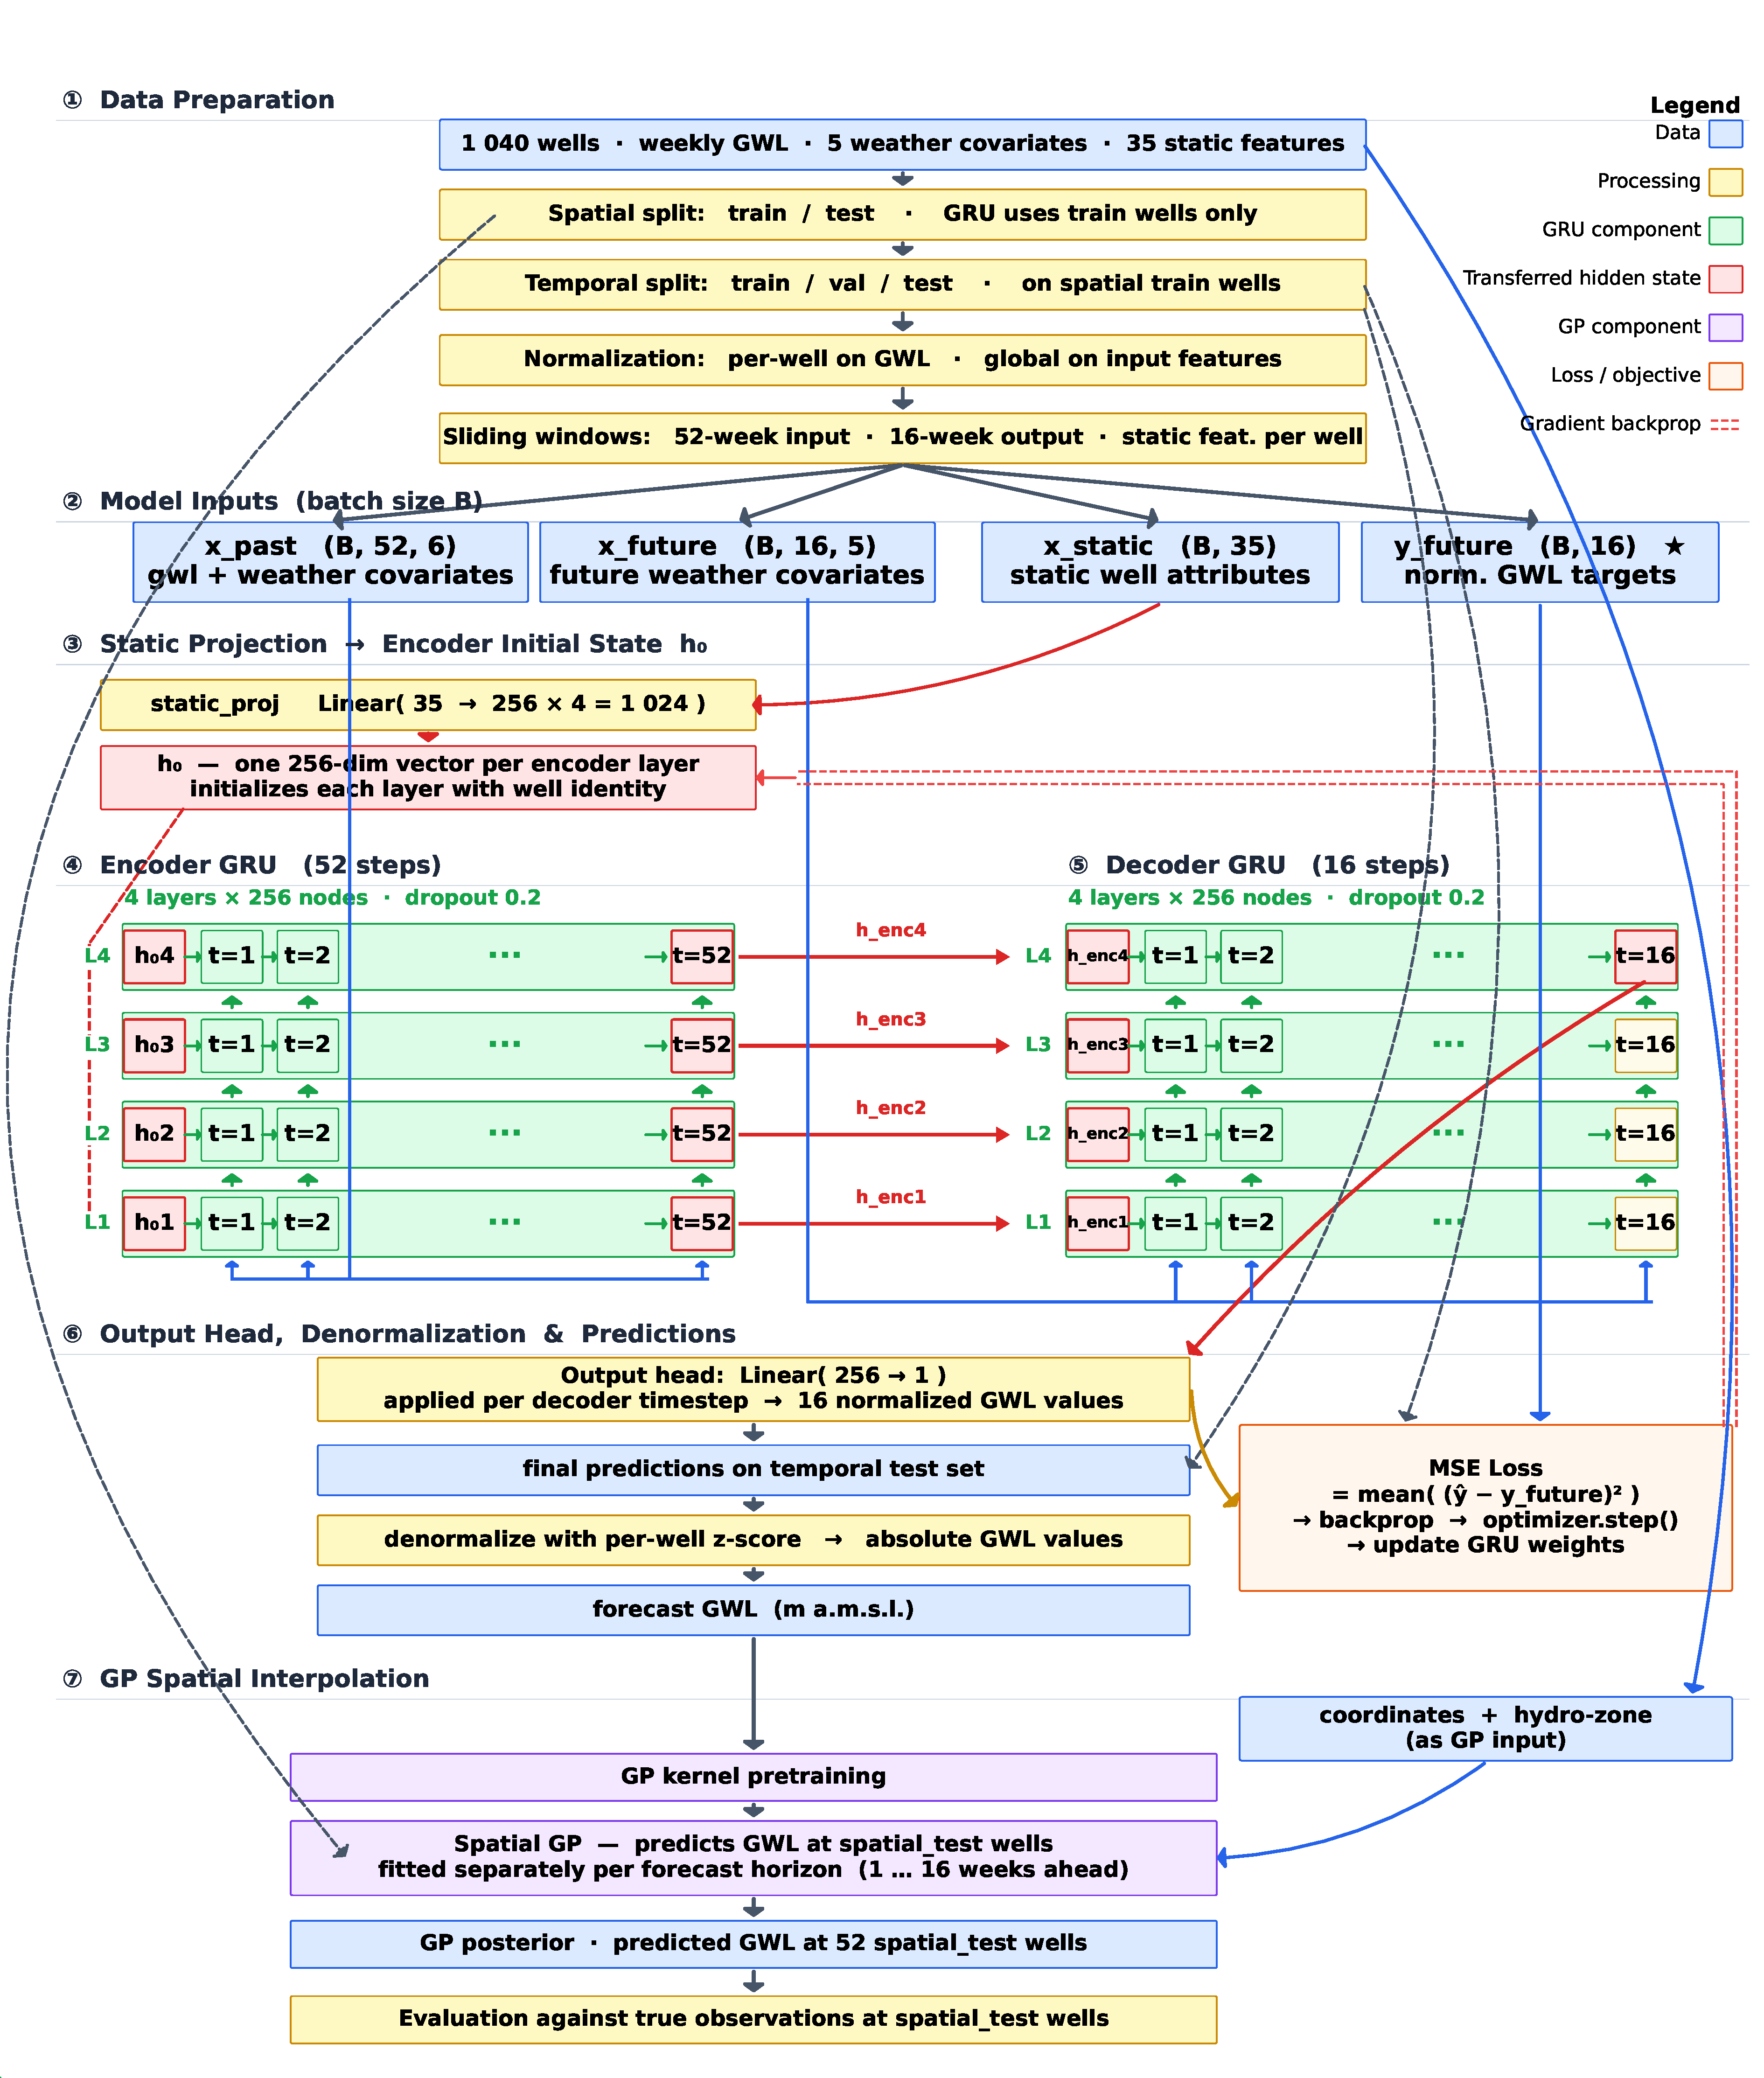
\includegraphics[width=\textwidth]{decoupled_flowchart_v2}
  \caption{Full two-stage spatiotemporal pipeline architecture (sections \textcircled{\small 1}–\textcircled{\small 7}). The GRU forecasts GWL at
  training wells (sections \textcircled{\small 1}–\textcircled{\small 6}); the GP then spatially interpolates those forecasts to
  test wells (section \textcircled{\small 7}). Both components are trained independently.}
  \label{fig:twostage_pipeline}
\end{figure}

\begin{figure}[p]
  \centering
  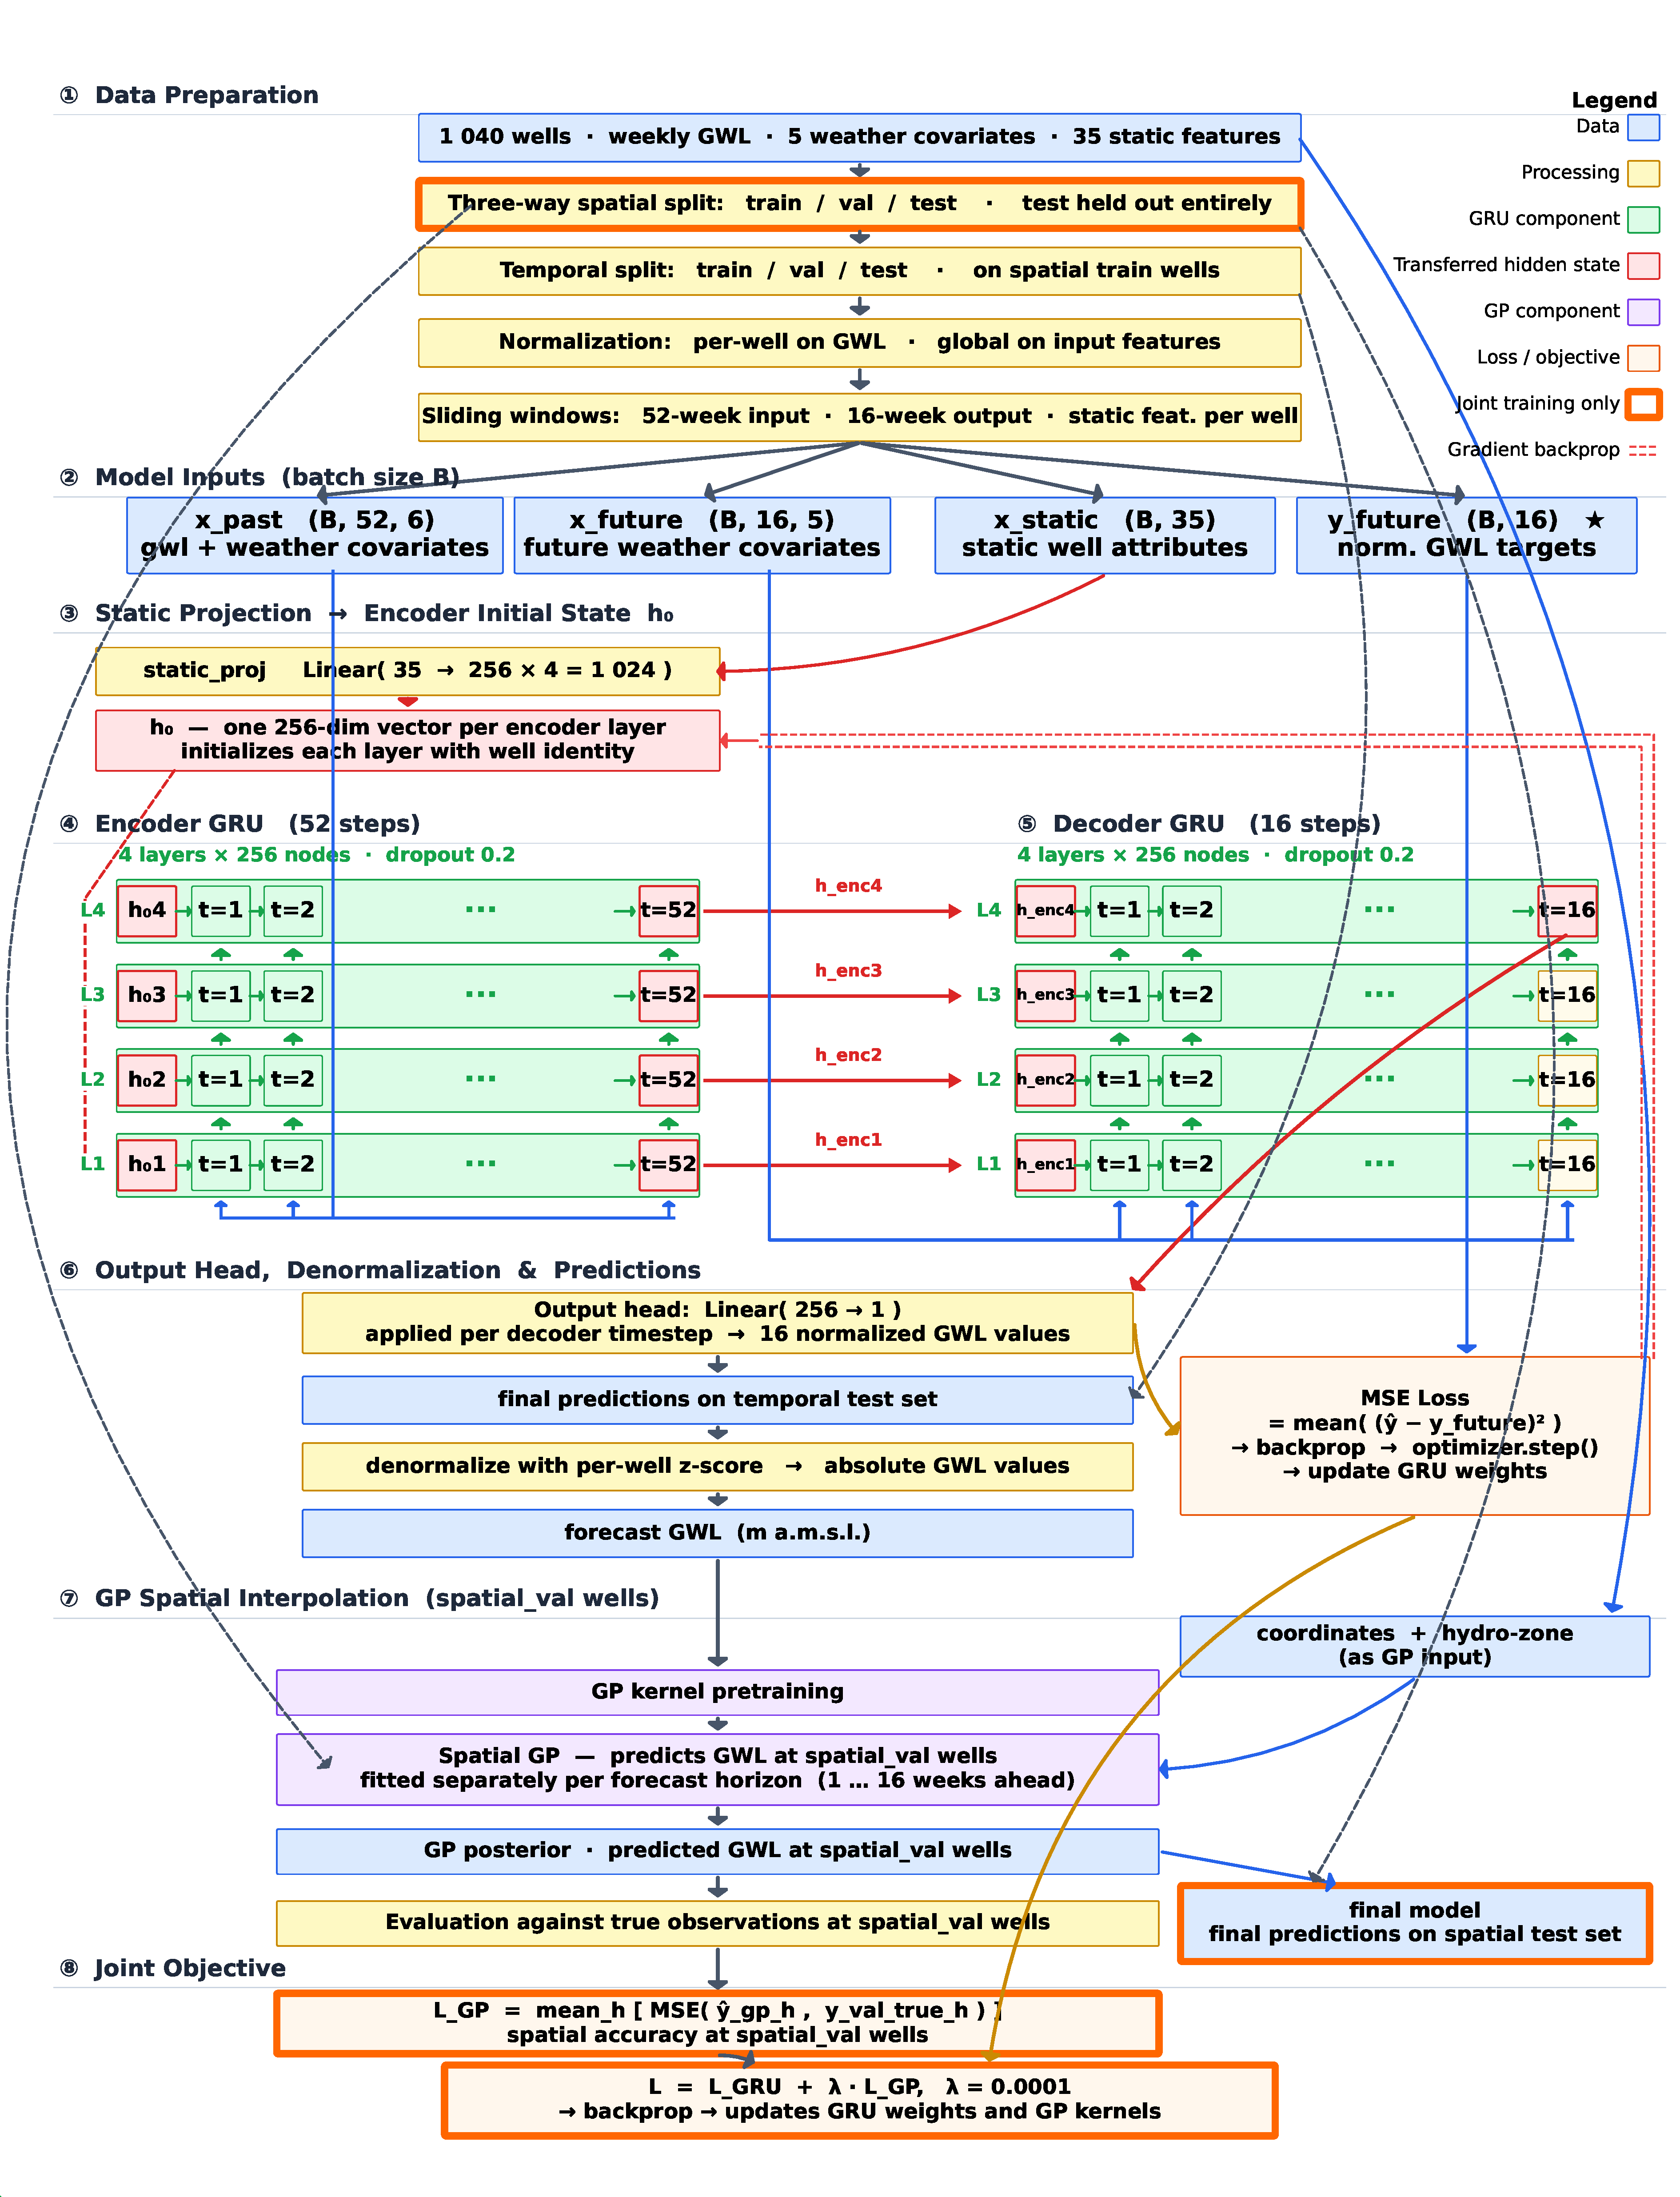
\includegraphics[width=\textwidth]{joint_flowchart_v3}
  \caption{Jointly trained spatiotemporal model (sections \textcircled{\small 1}–\textcircled{\small 8}). GRU and GP are trained end-to-end
  with a combined loss $\mathcal{L} = \mathcal{L}_{\text{GRU}} + \lambda \cdot \mathcal{L}_{\text{GP}}$
  ($\lambda = 0.0001$), combining GRU temporal MSE with GP spatial MSE at validation wells.
  The GP is conditioned on GRU predictions, so backpropagating $\mathcal{L}_{\text{GP}}$
  returns gradients to the GRU. A three-way well split is required: GRU training wells, GP
  spatial validation wells, and test wells.}
  \label{fig:joint_pipeline}
\end{figure}

% ============================================================
\section{Implementation}
\label{sec:implementation}
% ============================================================

The full implementation is available at \url{https://github.com/calgo-lab/gist}.

% ------------------------------------------------------------
\subsection{Software Stack}
\label{sec:software}
% ------------------------------------------------------------

The implementation uses Python 3.12 throughout. The GRU temporal model is implemented in
PyTorch \citep{paszke2019pytorch}, using standard \texttt{nn.GRU} layers with a custom
sequence-to-sequence wrapper and static-feature initialization of the encoder hidden state.
The Gaussian Process is implemented using GPyTorch \citep{gardner2018gpytorch} with exact
inference via Cholesky factorisation, as described in \cref{subsec:gp_background}.

Hyperparameter optimization is managed via iterative grid search, as described in \cref{subsec:hpo}.
Data preprocessing, feature engineering, and experiment tracking are handled with NumPy,
Pandas, and a lightweight custom experiment registry. Visualisation uses Matplotlib and
Seaborn.

% ------------------------------------------------------------
\subsection{Compute Infrastructure}
\label{sec:compute}
% ------------------------------------------------------------

All training and evaluation experiments are run on NVIDIA A100, H100, and H200 GPUs
provided through the Data Science Kubernetes cluster at Berliner Hochschule für Technik (BHT). Each job runs inside a Docker container built
from a custom image that pins the exact Python, PyTorch, and CUDA versions, ensuring that
all experiments are fully reproducible regardless of which GPU node the cluster schedules
the job on. Jobs are submitted via YAML-configured workloads specifying the container image,
resource requests, and entry point.

The GRU training runtime is roughly 20 minutes per job (50 epochs with early stopping,
1{,}040 wells, batch size 4096). GP kernel fitting (300 gradient-descent steps on the
marginal log-likelihood) is negligible in runtime; GP posterior evaluation (exact Cholesky
inference across all forecast dates and horizons) takes approximately 3 minutes per
split-seed. A full two-stage spatiotemporal pipeline job (1 GRU train + 1 GP evaluation)
therefore takes approximately 24 minutes; the true-observation interpolation baseline approximately 3 minutes. The jointly trained spatiotemporal model, which runs GRU and GP end-to-end in a single job, takes approximately 51 minutes
per run.

\Cref{tab:pipeline_efficiency} summarises the per-pipeline cluster job structure and
approximate runtimes per cluster job.

\begin{table}[htbp]
\centering
\begin{tabular}{lll}
\toprule
\textbf{Configuration} & \textbf{Steps per cluster job} & \textbf{Approx.\ time/job} \\
\midrule
Two-Stage Spatiotemporal Pipeline  & 1 GRU train $+$ 1 GP eval (gp\_seed 7) & $\approx$24\,min \\
True-Observation Interp.\ Baseline & 1 obs build $+$ 1 GP eval               & $\approx$3\,min \\
Jointly Trained Spatiotemporal Model & 1 joint training GRU+GP run              & $\approx$51\,min \\
Global GRU & 1 GRU train (1{,}040 wells, no test set) & $\approx$21\,min \\
\bottomrule
\end{tabular}
\caption{Cluster job structure and runtime for each model configuration}
\label{tab:pipeline_efficiency}
\end{table}

% ============================================================
\section{Chapter Summary}
% ============================================================

The GRU seq2seq model, Matérn-3/2 GP, and three pipeline variants are now fully specified. The evaluation protocol is fixed: a random 90/10 spatial split with a co-location constraint, repeated over 40 seeds, with hydrogeological zone as the sole GP feature (\cref{tab:pipeline_comparison}). Whether the two-stage pipeline actually benefits from the temporal forecasting step, and whether joint training helps at all, are open questions that \cref{ch:results} addresses empirically.

% Chapter 5 — Results
% !TEX root = ../main.tex
% ============================================================
%  Chapter 5 — Results
%  Factual findings only; interpretation is in Chapter 6.
% ============================================================

\chapter{Results}
\label{ch:results}

% ============================================================
\section{Experimental Setup}
\label{sec:exp_setup}
% ============================================================

All experiments use the configuration described in \cref{ch:methods}: the random 90/10 spatial split with 40 independent seeds, the GRU (h256/l4/do0.2), and the GP with Matérn-3/2 kernel and hydrogeological zone as the sole static feature. The primary reported metric is median per-well RMSE at $h=16$; IQR-normalized nRMSE\textsubscript{pw} is the primary metric for the GP feature ablation.
All experiments use HYRAS~5.0 reanalysis data for meteorological inputs, including the 16-week forecast horizon; reported error values therefore represent an upper bound on achievable performance under perfect meteorological information (see \cref{sec:limitations}).

% ============================================================
\section{GRU Temporal Performance}
\label{sec:gru_performance}
% ============================================================

\subsection{GRU vs.\ TFT: Replication Result}
\label{sec:gru_results}

To establish a TFT baseline, the training procedure from code shared directly
by the authors of \citet{kunz2025} is replicated on the Brandenburg dataset. This replication differs from
the original code in two ways. First, the original Kunz et al.\ code applies \texttt{fit\_transform} on the
validation set's static feature covariates; this replication corrects that by applying \texttt{transform},
which uses the scaler parameters estimated on the training set rather than refitting on the validation population.
Second, the original trains with distributed
data parallelism across four GPUs, for an effective batch size of
$4096 \times 4 = 16{,}384$; this replication uses a single GPU with batch size 4096.
Validation-loss early stopping (patience\,=\,5) is also added, which is not used in
the original.

With these changes, the replicated TFT achieves an h\,=\,16 RMSE of 0.089\,m,
compared to 0.093\,m from the original code the authors of \citet{kunz2025} shared
for the Brandenburg dataset, a 4.3\% improvement.

\Cref{tab:gru_vs_tft} compares both models on temporal forecasting at 1{,}040 monitored
training wells during the test period, using the same evaluation approach the authors of
\citet{kunz2025} apply to the Brandenburg dataset, with 10 seeds each. All values are
the median per well and then the mean across seeds; NSE uses the per-well test-period
mean as baseline (\cref{subsec:metrics}). The GRU reaches h\,=\,16 RMSE of 0.088\,m
and h\,=\,16 NSE of 0.764, matching the replicated TFT to within 0.001\,m, less than half
the GRU's seed-to-seed standard deviation (std\,$\approx$\,0.002\,m across 10 GRU seeds).
KGE at h\,=\,16 is 0.803 for the GRU and 0.814 for the TFT (\cref{tab:gru_vs_tft}),
which suggests the small RMSE gap does not reflect systematic bias or variability differences.
The roughly
90$\times$ training speedup (from about 31 hours to about 21 minutes on an A100 GPU on
the BHT Kubernetes cluster) is what makes the full experimental scope of this thesis
tractable: the HPO runs, feature ablations, multi-seed analysis, and joint training
experiments would all have been too slow at TFT training cost.

\begin{table}[htbp]
\centering
\resizebox{\textwidth}{!}{%
\begin{tabular}{lcccccccccc}
\toprule
 & \multicolumn{2}{c}{\textbf{RMSE (m)}} & \multicolumn{2}{c}{\textbf{NSE}} & \multicolumn{2}{c}{\textbf{IQR-nRMSE}} & \multicolumn{2}{c}{\textbf{KGE}} & \multicolumn{2}{c}{\textbf{vs.\ Kunz TFT}} \\
\cmidrule(lr){2-3}\cmidrule(lr){4-5}\cmidrule(lr){6-7}\cmidrule(lr){8-9}\cmidrule(lr){10-11}
\textbf{Model} & \textbf{h=16} & \textbf{avg} & \textbf{h=16} & \textbf{avg} & \textbf{h=16} & \textbf{avg} & \textbf{h=16} & \textbf{avg} & \textbf{$\Delta$ RMSE} & \textbf{$\Delta$ NSE} \\
\midrule
TFT \citep{kunz2025}          & 0.093 & 0.068 & 0.740 & 0.844 & 0.378 & 0.284 & 0.814 & 0.881 & ---        & ---       \\
TFT (replicated)              & 0.089 & 0.065 & 0.763 & 0.852 & 0.358 & 0.273 & 0.824 & 0.880 & $-4.3\%$   & $+3.1\%$  \\
Global GRU (h256/l4/do0.2)    & 0.088 & 0.066 & 0.764 & 0.852 & 0.371 & 0.284 & 0.803 & 0.869 & $-5.4\%$   & $+3.2\%$  \\
\bottomrule
\end{tabular}}
\caption{GRU vs.\ TFT: temporal performance (avg = mean over h=1-16; $\Delta$\,=\,\% change in h=16 metric relative to Kunz TFT)}
\label{tab:gru_vs_tft}
\end{table}

\begin{figure}[htbp]
  \centering
  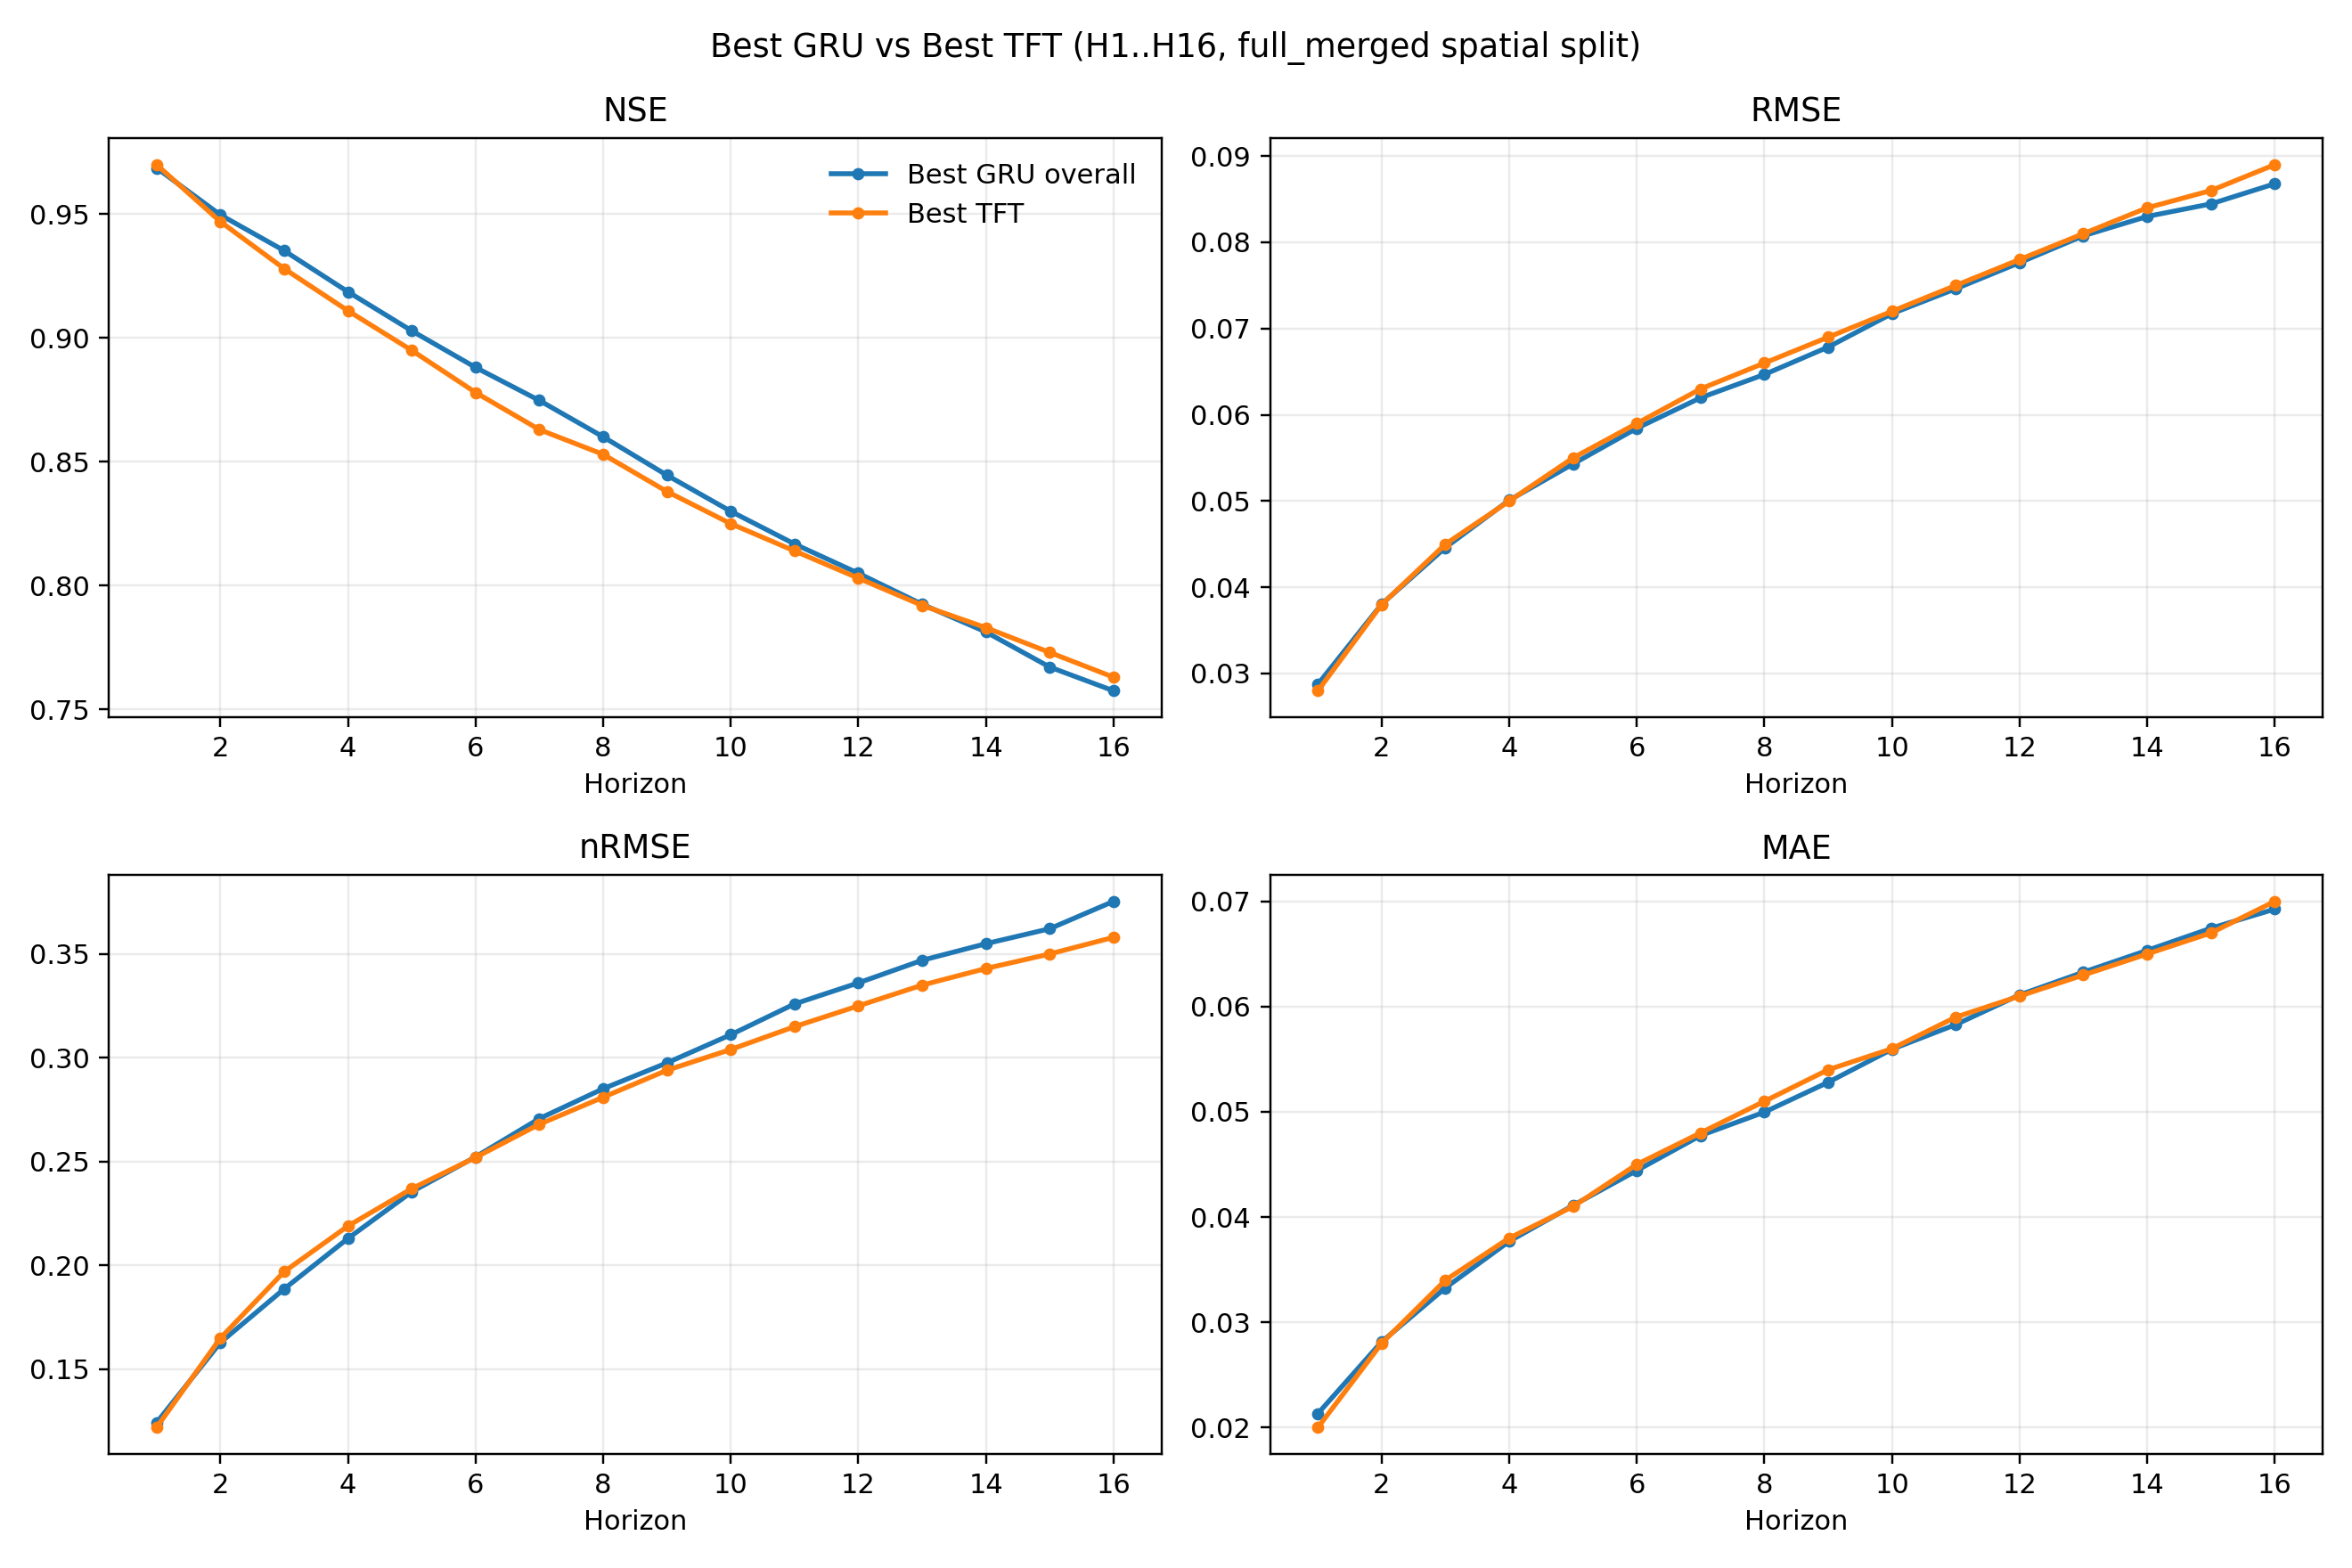
\includegraphics[width=0.85\textwidth]{gru_vs_tft}
  \caption{Per-metric comparison of best GRU and best TFT across forecast horizons H1-H16.
  Both models show near-identical NSE, RMSE, nRMSE, and MAE trajectories.}
  \label{fig:gru_vs_tft}
\end{figure}

\Cref{fig:scatter_gru_tft} shows the corresponding per-well RMSE and NSE at the training wells.

\begin{figure}[htbp]
  \centering
  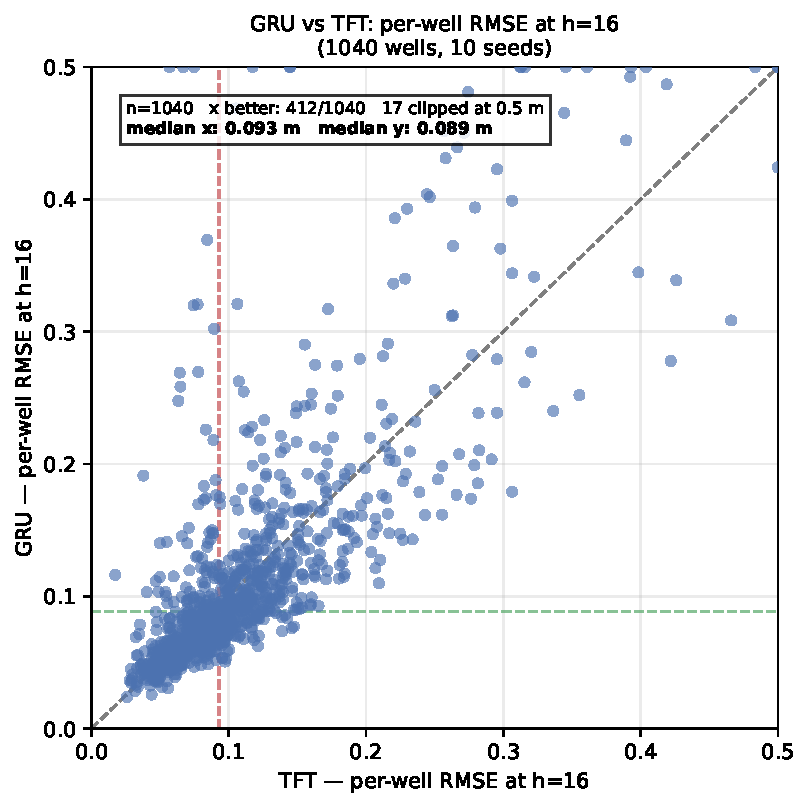
\includegraphics[width=0.48\textwidth]{scatter_rmse_gru_tft}
  \hfill
  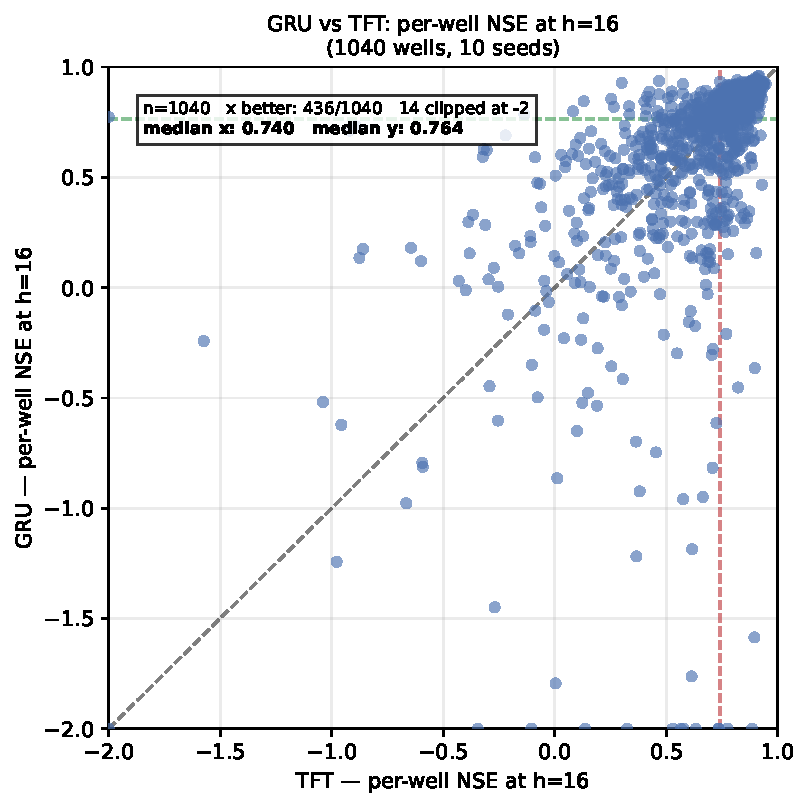
\includegraphics[width=0.48\textwidth]{scatter_nse_gru_tft}
  \caption{Per-well RMSE (left) and NSE (right): GRU vs.\ TFT at training wells (10 seeds each)}
  \label{fig:scatter_gru_tft}
\end{figure}

\subsection{GRU Feature Permutation Importance}
\label{sec:gru_feature_importance}

The Pardé seasonality coefficient dominates static feature importance ($+47.3\%$); temperature and precipitation dominate dynamic feature importance ($+91.5\%$ and $+84.5\%$ respectively). \Cref{tab:perm_importance,tab:perm_importance_dynamic} in \cref{app:additional_tables} report the full rankings.

The dominant feature, the Pardé seasonality coefficient ($+47.3\%$), captures the seasonal precipitation-response pattern for each well's catchment, and its contribution exceeds that of the next four highest-ranked features combined.

This dominance is specific to the h256/l4 architecture. An earlier analysis on a shallower h128/l5 model finds the Pardé seasonality coefficient to be harmful in that configuration, a discrepancy that likely reflects the h128/l5 model lacking sufficient capacity to condition correctly on seasonal response patterns across all 1{,}040 wells. The h256/l4 production runs retain the Pardé seasonality coefficient as an input; all 35 static features are included.

High permutation importance does not imply that a feature is essential. A GRU trained from scratch without the Pardé seasonality coefficient achieves essentially the same RMSE as one trained with it across 40 split seeds, within one seed-to-seed standard deviation. Permutation importance reflects how easy a feature is to exploit given the current model state, not how large its contribution to the final prediction could be if it were absent from training (\cref{tab:perm_importance,tab:perm_importance_dynamic}).

% ============================================================
\section{GP Feature Ablation}
\label{sec:gp_ablation}
% ============================================================

The GP feature ablation investigates the contribution of each static covariate to
interpolation performance. The true-observation interpolation baseline is used throughout: a GP
conditioned on true observed groundwater levels at training wells rather than GRU predictions.
This keeps each feature's contribution free of any influence from GRU forecast errors, and the
results transfer directly to the two-stage spatiotemporal pipeline since both use the same GP
kernel and feature encoding. The coordinate-only baseline (no static features) serves as the
reference point.

\paragraph{Ablation protocol.}
All 30 feature configurations are evaluated on the random 90/10 split using 10 split seeds
and 1 GP seed per configuration (300 GP evaluations in total). The configurations include
hydrogeological zone, aquifer confinement, groundwater residence time, well screen depths,
autocorrelation class, precipitation-response features, and groundwater level class, tested individually and in
combinations. All numbers reported here are means over 10 split seeds. Full results for all 30
configurations are in \cref{app:interp_baseline_ablation}.

The ablation uses IQR-normalized nRMSE\textsubscript{pw} as the primary metric. The 104
test wells cover a wide range of seasonal amplitudes (from $<$0.5\,m to $>$10\,m);
plain RMSE is dominated by high-amplitude wells, which carry more absolute error but respond
differently to static features than low-amplitude wells. IQR normalization gives each
well equal weight and produces a cleaner signal for feature selection.
RMSE\textsubscript{pw} is reported alongside for comparison.

\Cref{fig:gp_ablation_bar} summarises the relative performance of the core feature
configurations; \cref{tab:gp_ablation} shows the corresponding numerical values.

\begin{figure}[htbp]
  \centering
  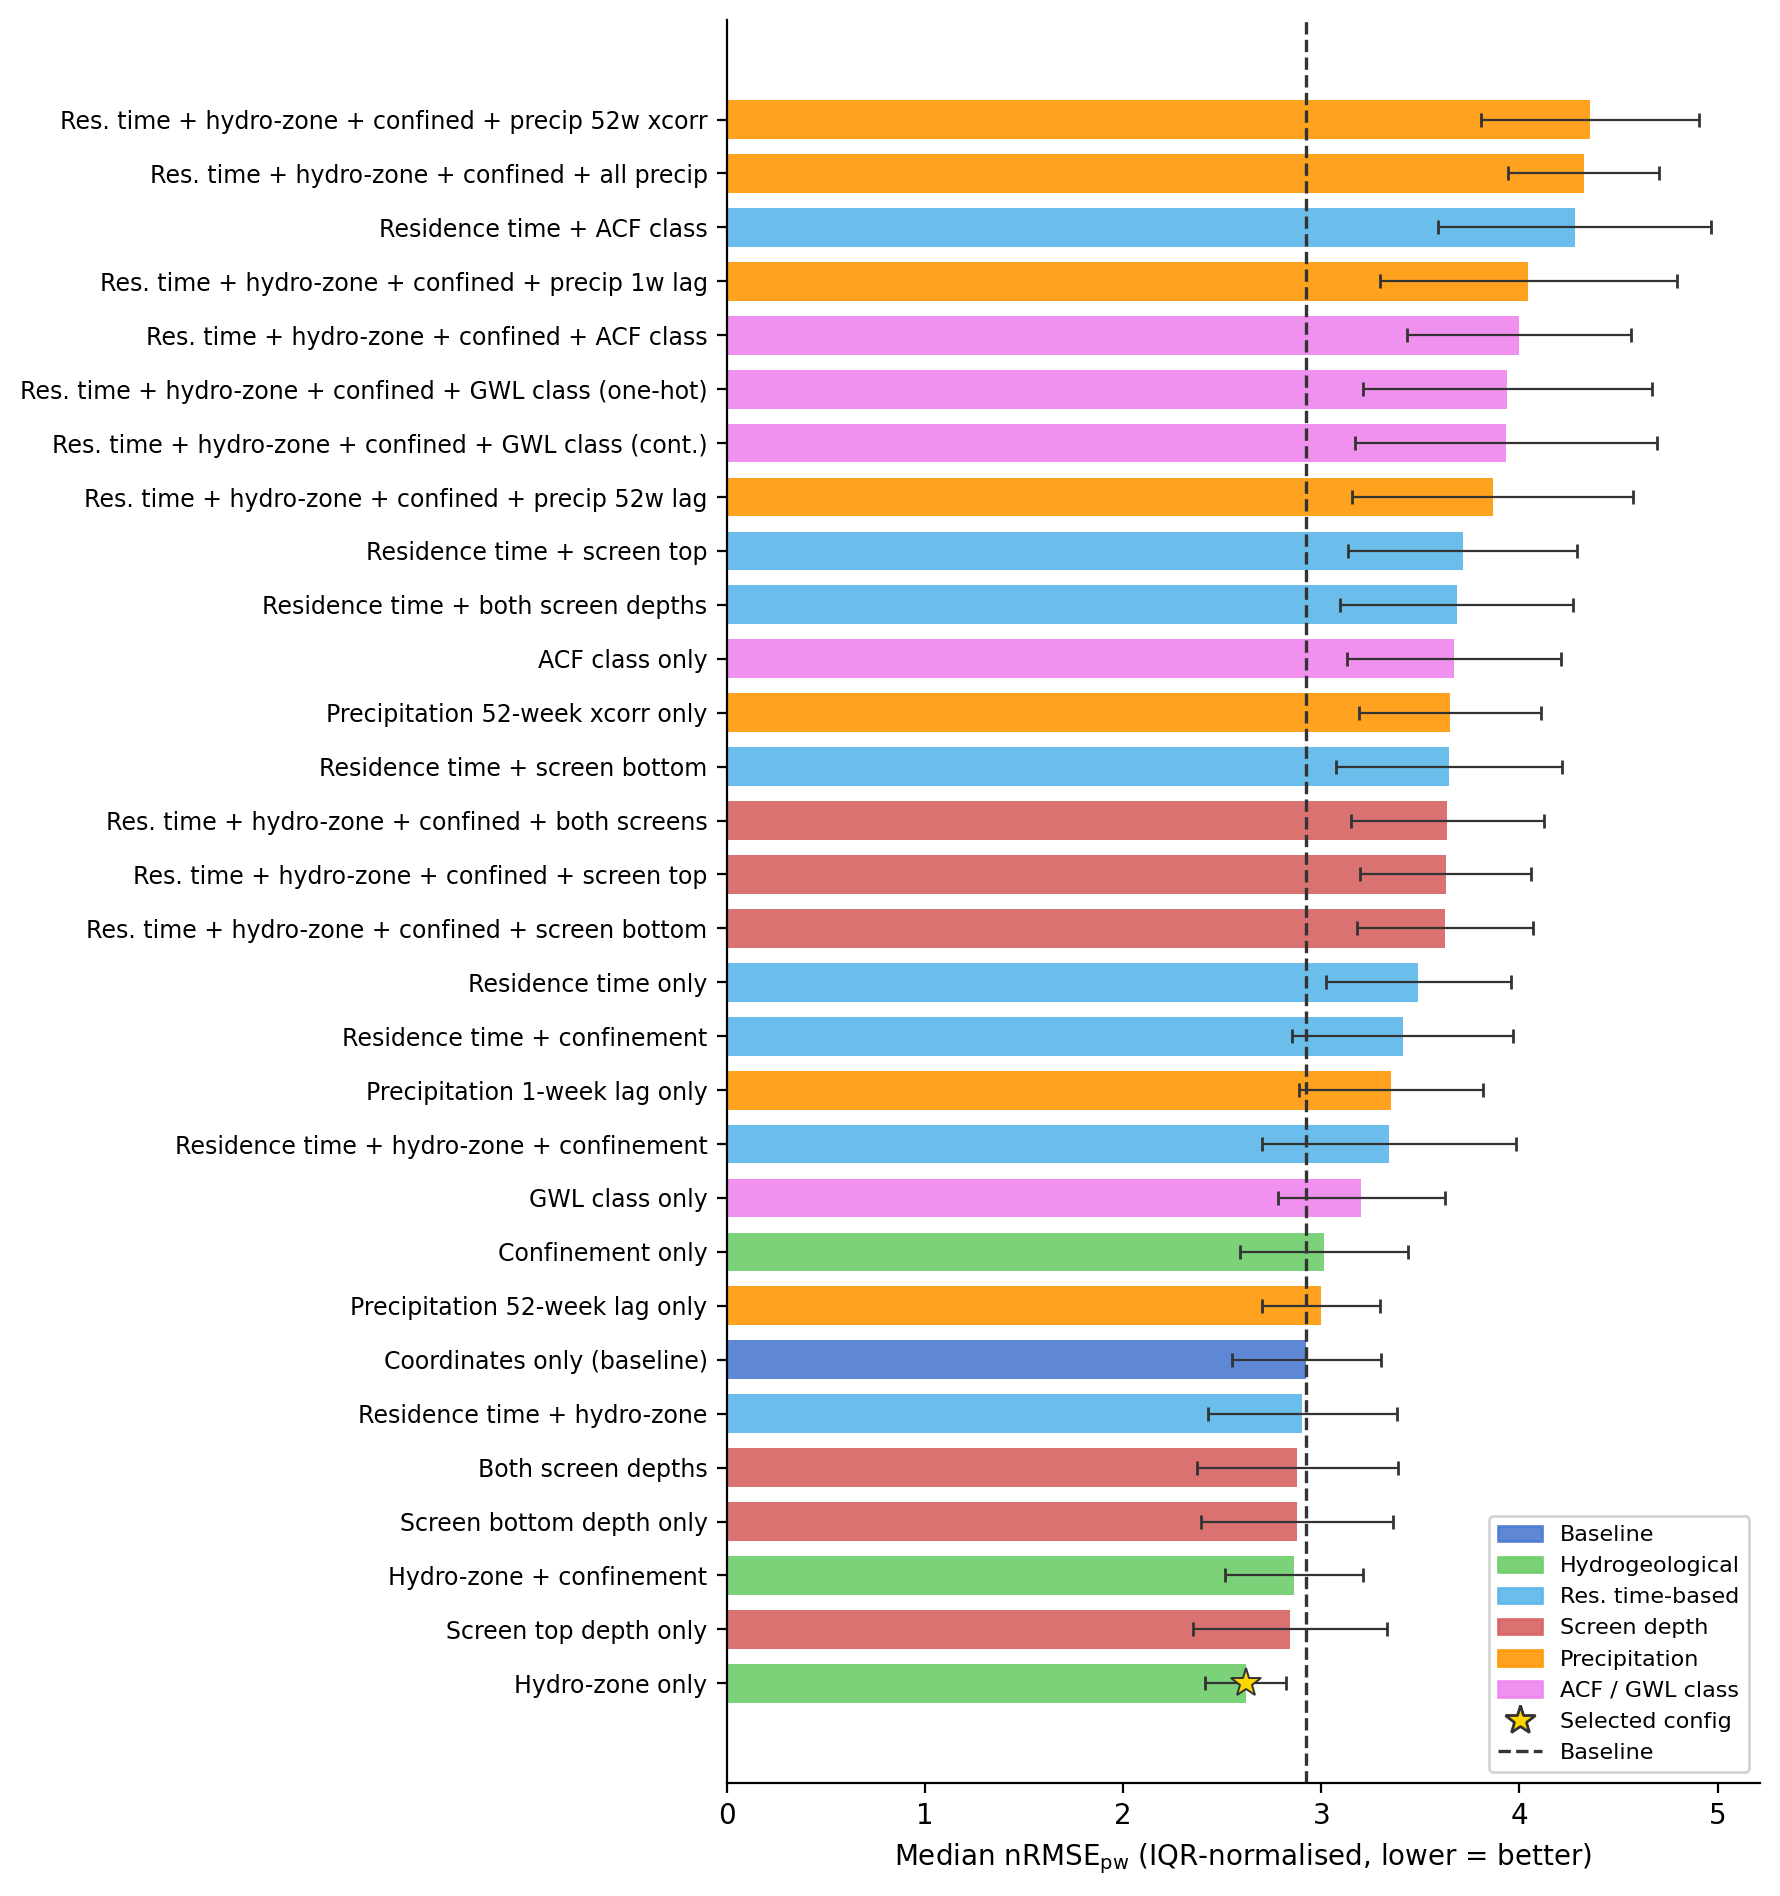
\includegraphics[width=0.85\textwidth]{gp_ablation_bar}
  \caption{GP feature ablation (IQR-nRMSE\textsubscript{pw}, lower is better; dashed line: coordinate-only baseline; star: selected configuration)}
  \label{fig:gp_ablation_bar}
\end{figure}

\begin{table}[htbp]
\centering
\begin{tabular}{lrrr}
\toprule
\textbf{Feature config} & \textbf{nRMSE} & \textbf{$\Delta$ nRMSE} & \textbf{RMSE (m)} \\
\midrule
\textbf{Hydrogeological zone only} $\star$    & \textbf{4.444} & $-$0.633 & \textbf{1.052} \\
Screen top depth only                        & 4.883          & $-$0.194 & 1.070 \\
Confinement only                             & 5.017          & $-$0.060 & 1.148 \\
\textit{Coordinates only (baseline)}         & 5.077          & ---      & 1.130 \\
Hydrogeological zone + confinement           & 5.207          & $+$0.130 & 1.153 \\
Residence time only                          & 5.437          & $+$0.361 & 1.261 \\
\bottomrule
\end{tabular}
\caption{GP feature ablation: selected configurations (median IQR-nRMSE\textsubscript{pw} and RMSE\textsubscript{pw}; lower is better; full table in \cref{app:interp_baseline_ablation})}
\label{tab:gp_ablation}
\end{table}

\paragraph{Hydrogeological zone only is the selected configuration.}
The hydrogeological zone feature (one-hot encoded from three classes:
recharge, transit, and discharge zones) achieves the largest reduction in
IQR-normalized nRMSE\textsubscript{pw}: $-$0.633 ($-$12.5\%) relative to the
coordinate-only baseline. No other single feature comes close: the next-best configurations
show gains of only $-$0.060 to $-$0.194 on IQR-nRMSE\textsubscript{pw}, all within one seed-to-seed standard deviation of the
baseline, while the winning gap of $-$0.633 is more than three times the next-best gain. All precipitation-response features, residence time, and the autocorrelation class hurt
performance. The selected configuration also achieves the best RMSE\textsubscript{pw} simultaneously, winning on both metrics.

The nRMSE result is stronger than the corresponding RMSE comparison. The RMSE reduction is
only $-$0.078\,m ($-$6.9\%), which is small relative to the seed-to-seed spread
(std\,$\approx$\,0.16\,m across 10 seeds).
The difference between metrics is also visible in the rankings: confinement only ranks third on
nRMSE ($\Delta = -0.060$) yet slightly worsens RMSE relative to the coordinate-only baseline
($+$0.018\,m). Adding confinement to hydrogeological zone together is worse than hydrogeological zone alone on both metrics,
with nRMSE increasing by $+$0.130 relative to the baseline.

\paragraph{Dynamic meteorological features.}
Temperature, precipitation, and relative humidity are tested on top of the best
static configuration (hydrogeological zone only) using the true-observation interpolation baseline on the random 90/10 split,
10 split seeds and one GP seed per configuration (10 evaluations each). \Cref{tab:gp_ablation_dynamic}
reports the results.
All three dynamic features increase median nRMSE\textsubscript{pw} relative to the baseline
(4.44): temperature by $+0.54$ ($+12\%$), relative humidity by $+0.98$ ($+22\%$), and
precipitation by $+2.19$ ($+49\%$). Adding all three together does not improve over
precipitation alone. The GP spatial kernel does not benefit from time-varying meteorological
inputs, which is consistent with the kernel capturing spatial rather than temporal structure.
Dynamic meteorological features are not added to the final GP configuration.

\begin{table}[htbp]
\centering
\begin{tabular}{lrr}
\toprule
\textbf{Feature config}             & \textbf{nRMSE (mean $\pm$ std)} & \textbf{$\Delta$} \\
\midrule
\textit{Hydrogeological zone only (baseline)}  & $4.44 \pm 0.50$                 & ---       \\
Hydrogeological zone + temperature            & $4.98 \pm 1.06$                 & $+$0.54   \\
Hydrogeological zone + relative humidity      & $5.43 \pm 1.12$                 & $+$0.98   \\
Hydrogeological zone + precipitation          & $6.64 \pm 1.29$                 & $+$2.19   \\
Hydrogeological zone + all three met          & $6.63 \pm 1.26$                 & $+$2.19   \\
\bottomrule
\end{tabular}
\caption{GP dynamic feature ablation (median IQR-nRMSE\textsubscript{pw} per well, mean over 10 split seeds; lower is better)}
\label{tab:gp_ablation_dynamic}
\end{table}

\paragraph{Matérn-5/2 kernel.}
The default kernel is Matérn-3/2. To check whether a smoother kernel would improve spatial interpolation, the true-observation interpolation baseline is re-run with Matérn-5/2 ($\nu=2.5$) on the random 90/10 split (10 split seeds, 1 GP seed, hydrogeological zone only). \Cref{tab:matern_kernel_comparison} shows the comparison: Matérn-5/2 gives RMSE\textsubscript{pw} of $1.235 \pm 0.163$\,m vs.\ $1.052 \pm 0.160$\,m for Matérn-3/2. The smoother kernel is worse by 0.18\,m on average (17.4\%), which confirms Matérn-3/2 as the better choice.

\begin{table}[htbp]
\centering
\begin{tabular}{lc}
\toprule
\textbf{Kernel} & \textbf{RMSE\textsubscript{pw} (m)} \\
\midrule
Matérn-3/2 $\star$ & $1.052 \pm 0.160$ \\
Matérn-5/2          & $1.235 \pm 0.163$ \\
\bottomrule
\end{tabular}
\caption{Matérn 3/2 vs.\ 5/2 kernel comparison for GP}
\label{tab:matern_kernel_comparison}
\end{table}

% ============================================================
\section{Main Pipeline Results}
\label{sec:main_pipeline_results}
% ============================================================

\subsection{Two-Stage Spatiotemporal Pipeline}
\label{sec:twostage_performance}

The two-stage spatiotemporal pipeline is evaluated on the primary random 90/10 split using
40 split seeds (ss42--ss81), 1 GRU seed, 1 GP seed, the co-location-aware sampling algorithm, and
hydrogeological zone only as the GP feature. The full metric comparison across all five model
configurations is in \cref{tab:pipeline_main}; the discussion here focuses on the two-stage
pipeline's key results.

\subsection{Two-Stage Pipeline and Interpolation Baseline}
\label{sec:bottleneck}

At h\,=\,16, the two-stage pipeline RMSE of 1.082\,m (\cref{tab:pipeline_main}) is roughly 12$\times$ the GRU temporal RMSE of 0.088\,m (\cref{tab:gru_vs_tft}).

The two-stage pipeline achieves a mean per-well RMSE of $1.119 \pm 0.208$\,m and an
IQR-normalized nRMSE\textsubscript{pw} of $4.580 \pm 0.909$ (means $\pm$ std across 40
seeds). The true-observation interpolation baseline achieves $1.116 \pm 0.208$\,m. The seed-to-seed standard deviation of the per-seed median gap is 0.033\,m; dividing by $\sqrt{40}$ (for 40 split seeds) gives a standard error of 0.005\,m. The observed mean gap of 0.003\,m (less than 0.3\%) is smaller than one standard error. A paired $t$-test across the 40 seeds gives $t_{39} = 0.68$, $p = 0.50$: if the true gap were zero, random sampling would produce a $t$-statistic at least this large 50\% of the time, so the two configurations are effectively equal on this metric. \Cref{fig:scatter_oracle_vs_decoupled} shows the per-well RMSE comparison. The GP's 95\% nominal prediction intervals achieve approximately 60\% empirical coverage (mean $0.602 \pm 0.043$ across 40 seeds; PICP) at the spatial test wells (\cref{sec:limitations}).
\begin{figure}[htbp]
  \centering
  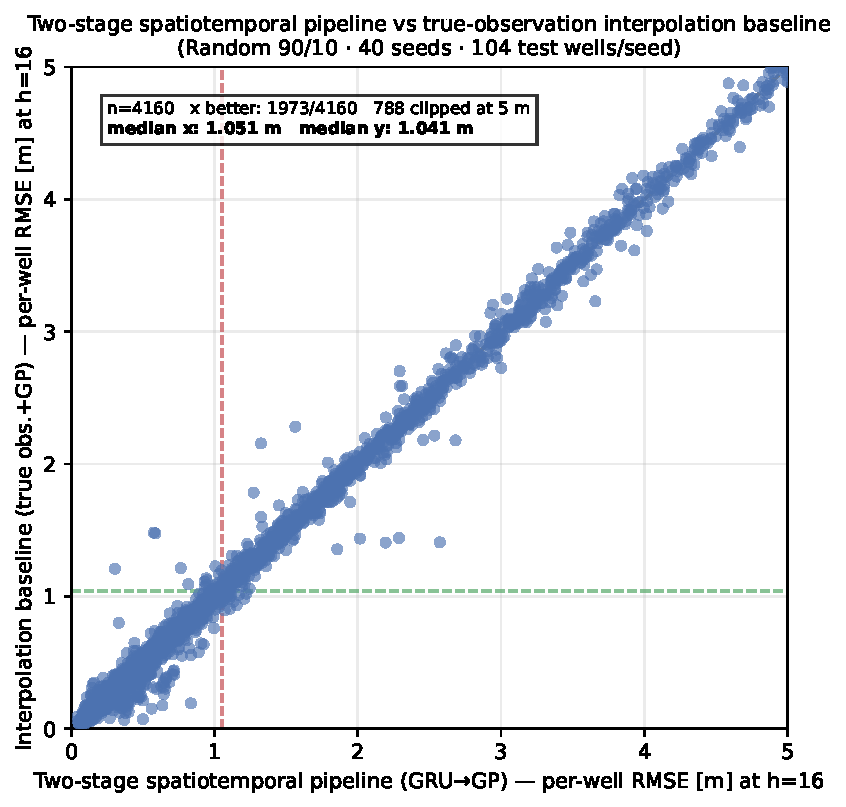
\includegraphics[width=0.60\textwidth]{scatter_rmse_oracle_vs_decoupled}
  \caption{Per-well RMSE: interpolation baseline vs.\ two-stage pipeline (random 90/10, 40 seeds; n\,=\,4{,}160 (well, seed) pairs)}
  \label{fig:scatter_oracle_vs_decoupled}
\end{figure}

% ============================================================
\section{Spatiotemporal Pipeline Comparison}
\label{sec:pipeline_comparison}
% ============================================================

\Cref{tab:pipeline_main} compares four model configurations on the primary random 90/10 split
(40 split seeds, co-location-aware sampling): one temporal baseline (Global GRU)
and three spatiotemporal pipeline variants (1 GP seed, hydrogeological zone only).

GRU metrics are evaluated at monitored training wells during the test period and are not
directly comparable to the GP pipeline metrics at 104 unseen test wells.
The Interp.\ Baseline uses true observed GWL as GP input and gives an upper bound on
pipeline performance.

\begin{table}[htbp]
\centering
\begin{tabular}{lcccc}
\toprule
\textbf{Configuration} & \textbf{h=16 RMSE (m)} & \textbf{avg RMSE (m)} & \textbf{h=16 NSE} & \textbf{avg NSE} \\
\midrule
Global GRU (h256/l4/do0.2) & $0.089 \pm 0.002$ & $0.069 \pm 0.002$ & $0.765 \pm 0.011$ & $0.849 \pm 0.008$ \\
\midrule
Two-Stage (GRU+GP)          & $1.082 \pm 0.193$ & $1.119 \pm 0.208$ & $-32.9 \pm 16.4$ & $-38.4 \pm 16.9$ \\
Interp.\ Baseline           & $1.079 \pm 0.191$ & $1.116 \pm 0.208$ & $-33.1 \pm 16.9$ & $-38.6 \pm 17.1$ \\
Jointly Trained             & $1.259 \pm 0.290$ & $1.286 \pm 0.278$ & $-46.1 \pm 30.8$ & $-52.1 \pm 32.8$ \\
\bottomrule
\end{tabular}
\caption{Pipeline comparison, random 90/10 split (40 seeds). Per-well NSE is expected to be strongly negative for all spatial pipeline variants; see \cref{subsec:metrics} for the structural reason and \cref{subsec:global_metrics} for the contrast with global NSE.}
\label{tab:pipeline_main}
\end{table}

\Cref{fig:scatter_rmse_rand} shows per-well RMSE comparing the global GRU temporal model against the two-stage pipeline.

\begin{figure}[htbp]
  \centering
  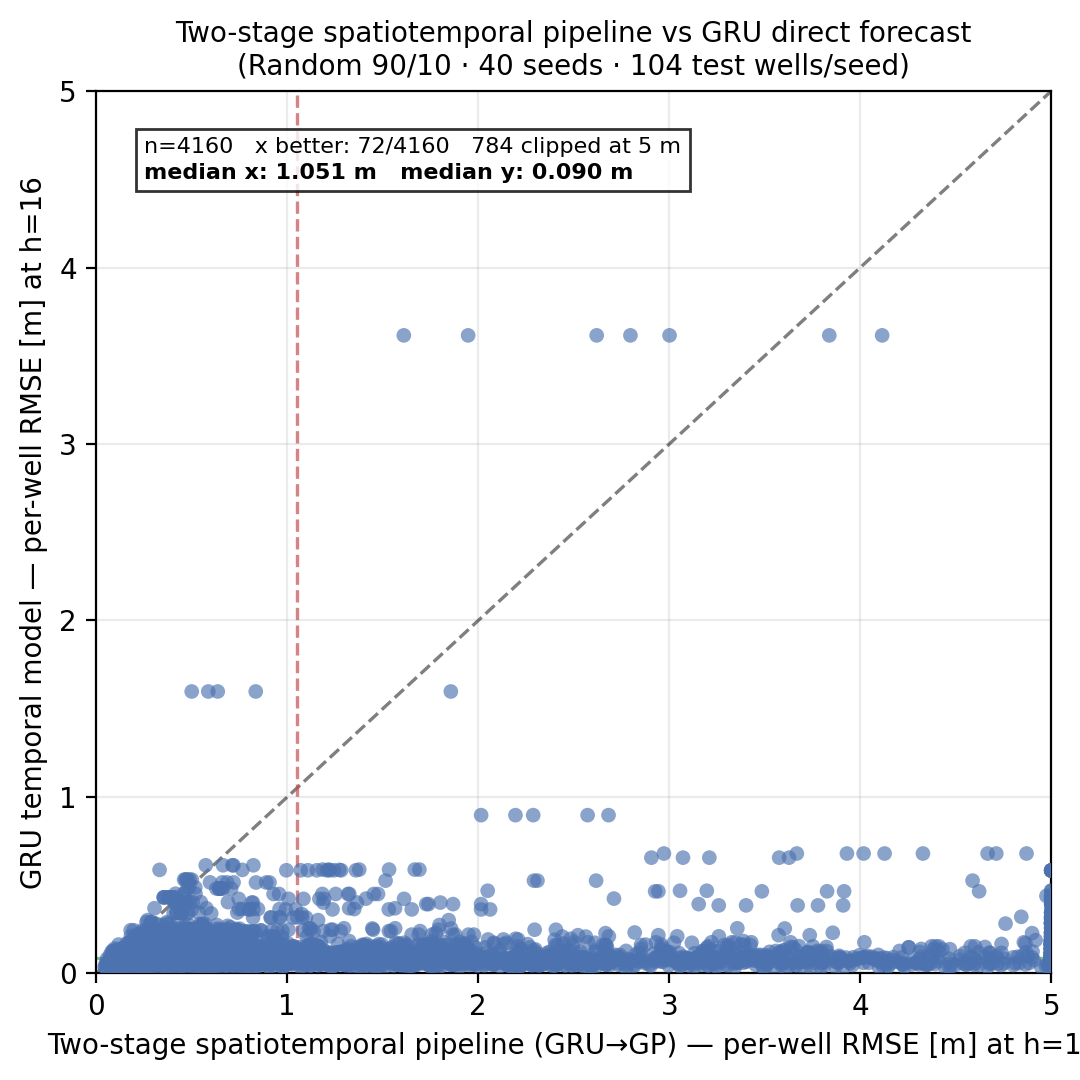
\includegraphics[width=0.75\textwidth]{scatter_rmse_rand}
  \caption{Per-well RMSE: GRU temporal (y-axis) vs.\ two-stage pipeline (x-axis), random split (40 seeds)}
  \label{fig:scatter_rmse_rand}
\end{figure}

\Cref{fig:rmse_by_horizon} shows median per-well RMSE across forecast horizons H1--H16 for all three pipeline configurations. All three show broadly flat profiles.

\begin{figure}[htbp]
  \centering
  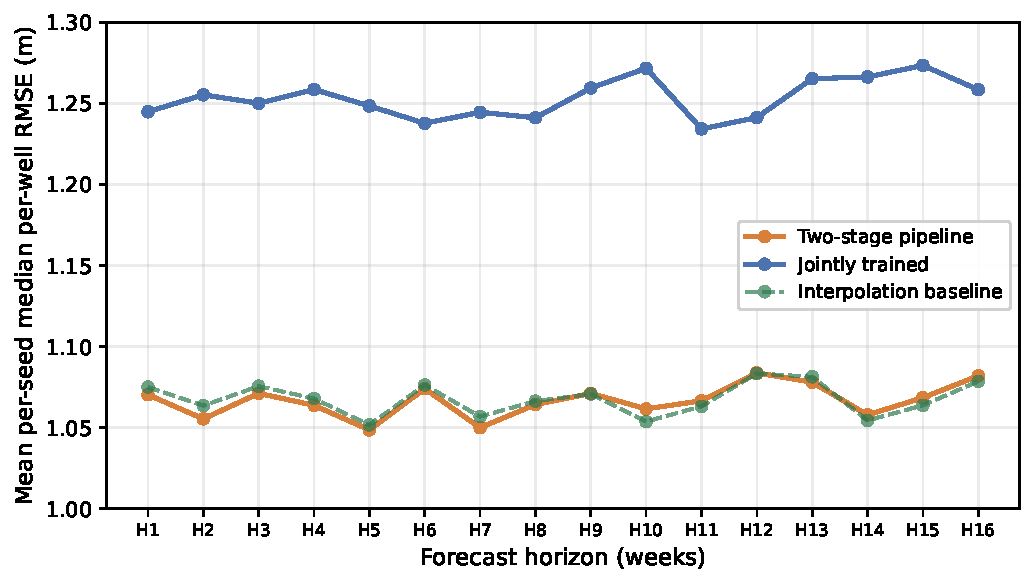
\includegraphics[width=0.85\textwidth]{horizon_pipeline_comparison}
  \caption{Median per-well RMSE by forecast horizon (random 90/10, 40 seeds; all three pipeline configurations)}
  \label{fig:rmse_by_horizon}
\end{figure}

\subsection{Joint Training}
\label{sec:joint_results}

The jointly trained spatiotemporal model takes roughly twice as long to train as the two-stage pipeline and produces worse results on average: mean per-seed median h\,=\,16 RMSE is 1.259\,m vs.\ 1.082\,m for the two-stage pipeline (16.4\% higher).

\Cref{fig:perwell_rmse_scatter} shows per-well RMSE for all 4{,}160 (well, seed) pairs across the 40 seeds, clipped at 5\,m. The two-stage pipeline is better for 2{,}199 of 4{,}160 pairs.

\begin{figure}[htbp]
  \centering
  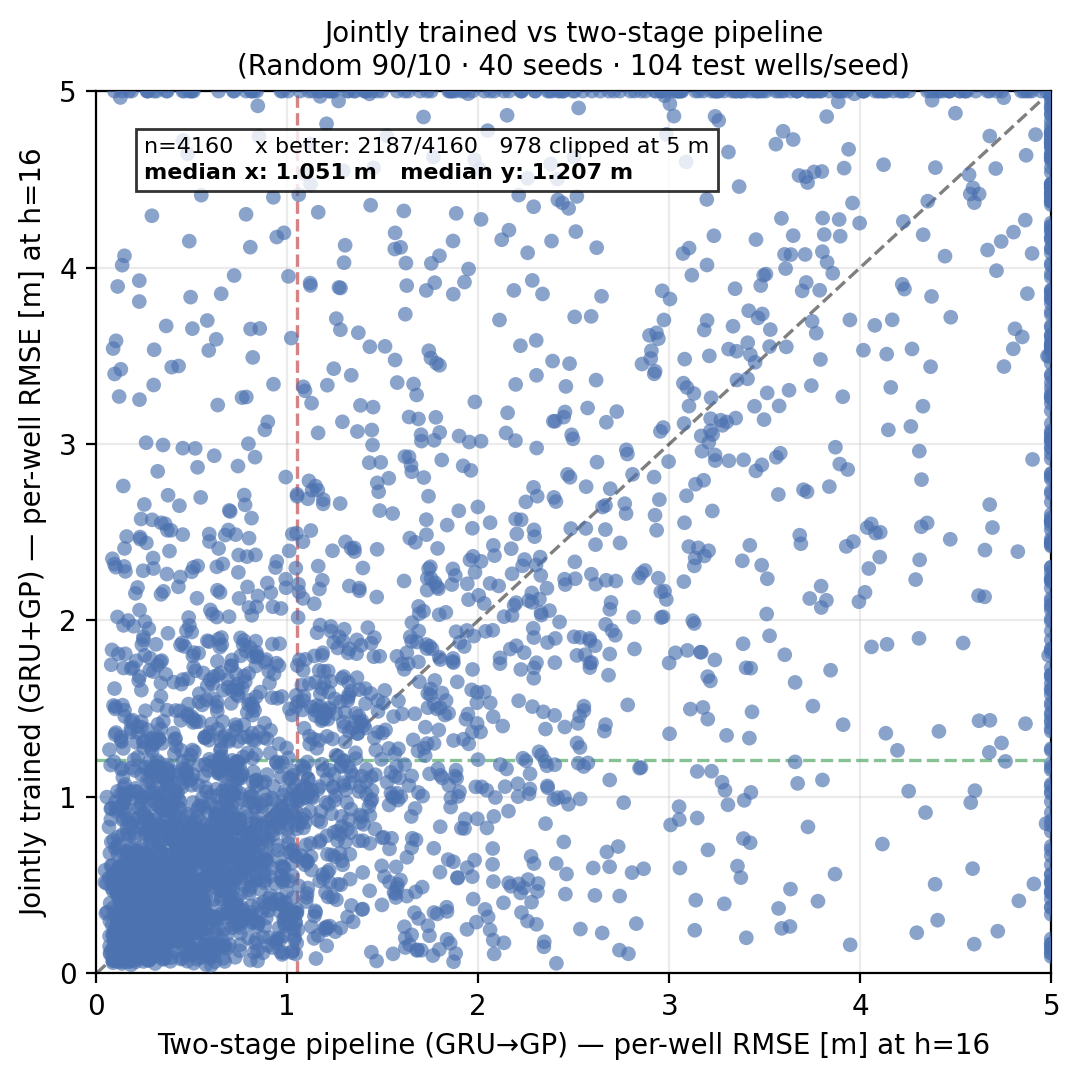
\includegraphics[width=0.75\textwidth]{perwell_rmse_scatter}
  \caption{Per-well RMSE: two-stage vs jointly trained (random 90/10, 40 seeds; n\,=\,4{,}160 (well, seed) pairs; axis clipped at 5\,m; two-stage better for 2{,}199/4{,}160 pairs)}
  \label{fig:perwell_rmse_scatter}
\end{figure}

But the per-well breakdown tells a different story: the jointly trained model is worse for close wells and better for the most isolated ones (see \cref{sec:distance_error}).


% ============================================================
\section{Distance-Error Relationship}
\label{sec:distance_error}
% ============================================================

Distance between a test well and its nearest training neighbor is the primary driver of
interpolation difficulty. This holds both across seeds and within seeds.

\subsection{Across Seeds: Spearman Correlation}

The random split exhibits substantial standard deviation across 40 seeds. The full per-seed
breakdown of median nearest-training-well distance and RMSE\textsubscript{pw} is in
\cref{tab:seed_distance} (Appendix~B). Seeds that draw more spatially isolated test wells
show higher RMSE: the Spearman correlation between median nearest-training-well distance and
per-seed median RMSE is $\rho = 0.603$ ($p < 0.001$, $n = 40$, $t = 4.66$, $df = 38$).
\Cref{fig:distance_rmse} shows this relationship: each point is one of the 40 seeds,
with its median nearest-training-well distance on the $x$-axis and its median two-stage
pipeline RMSE on the $y$-axis.

\begin{figure}[htbp]
  \centering
  
\includegraphics[width=0.85\textwidth]{seed_distance_scatter}
  \caption{Median RMSE vs.\ median nearest-training-well distance across 40 seeds (random 90/10 split; Spearman $\rho = 0.603$, $p < 0.001$)}
  \label{fig:distance_rmse}
\end{figure}

\subsection{Distance-Binned RMSE}

\Cref{fig:ntn_km_rmse} shows median per-well RMSE in 1\,km distance bins for both pipeline variants, pooled across 40 seeds. Below 2.5\,km, the two-stage pipeline performs better. From roughly 4.5\,km onward
the ranking reverses: by the farthest distance bin (median distance 6.8\,km) the two-stage
pipeline reaches 5.4\,m against 4.3\,m for the jointly trained model. \Cref{fig:scatter_joint_close,fig:scatter_joint_far} confirm this at the extremes:
for the closest 10\% of test wells ($\leq 0.61$\,km, $n = 422$), the two-stage pipeline is
better on 282 of 422 pairs (median RMSE 0.675\,m vs.\ 1.098\,m for the jointly trained
model); for the farthest 10\% ($\geq 5.45$\,km, $n = 413$), the jointly trained model is
better on 282 of 413 pairs (median RMSE 4.261\,m vs.\ 5.369\,m for the two-stage pipeline).

\begin{figure}[htbp]
  \centering
  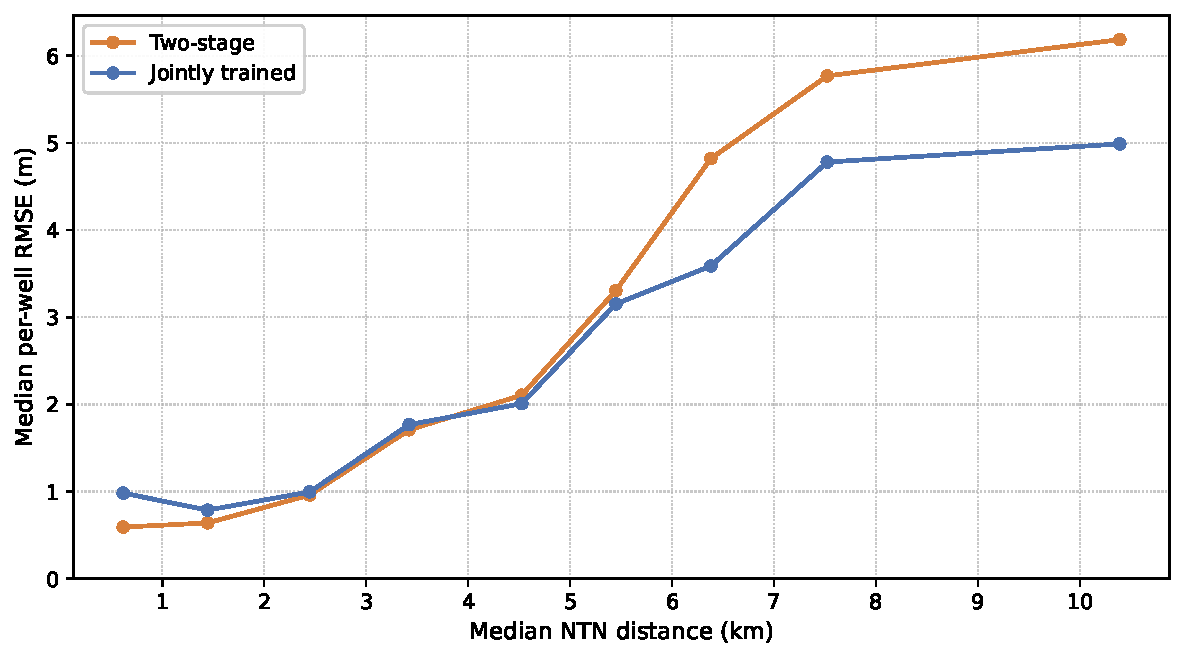
\includegraphics[width=0.85\textwidth]{ntn_km_rmse}
  \caption{Median per-well RMSE vs.\ nearest-training-well distance (km) for both pipeline variants (random 90/10, 40 seeds)}
  \label{fig:ntn_km_rmse}
\end{figure}

\begin{figure}[!htbp]
  \centering
  \subcaptionbox{Closest 10\% ($\leq 0.61$\,km)\label{fig:scatter_joint_close}}{%
    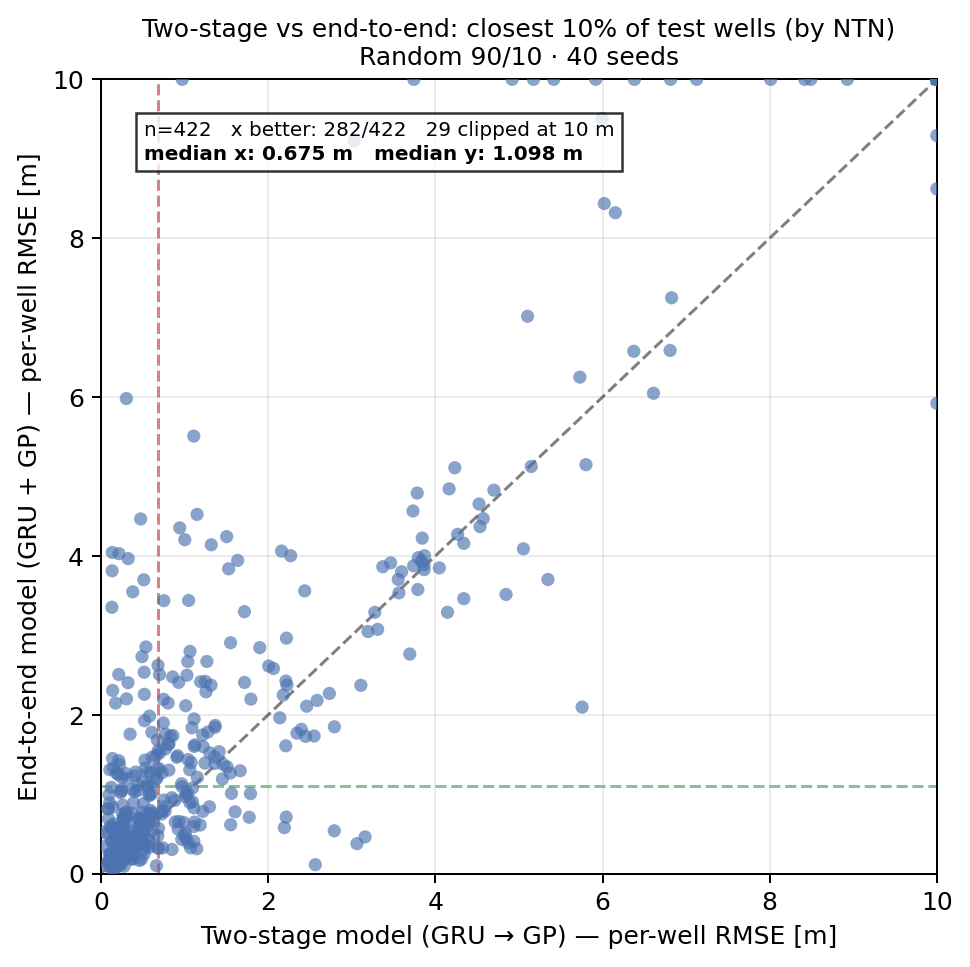
\includegraphics[width=0.47\textwidth]{scatter_main_close}}\hfill
  \subcaptionbox{Farthest 10\% ($\geq 5.45$\,km)\label{fig:scatter_joint_far}}{%
    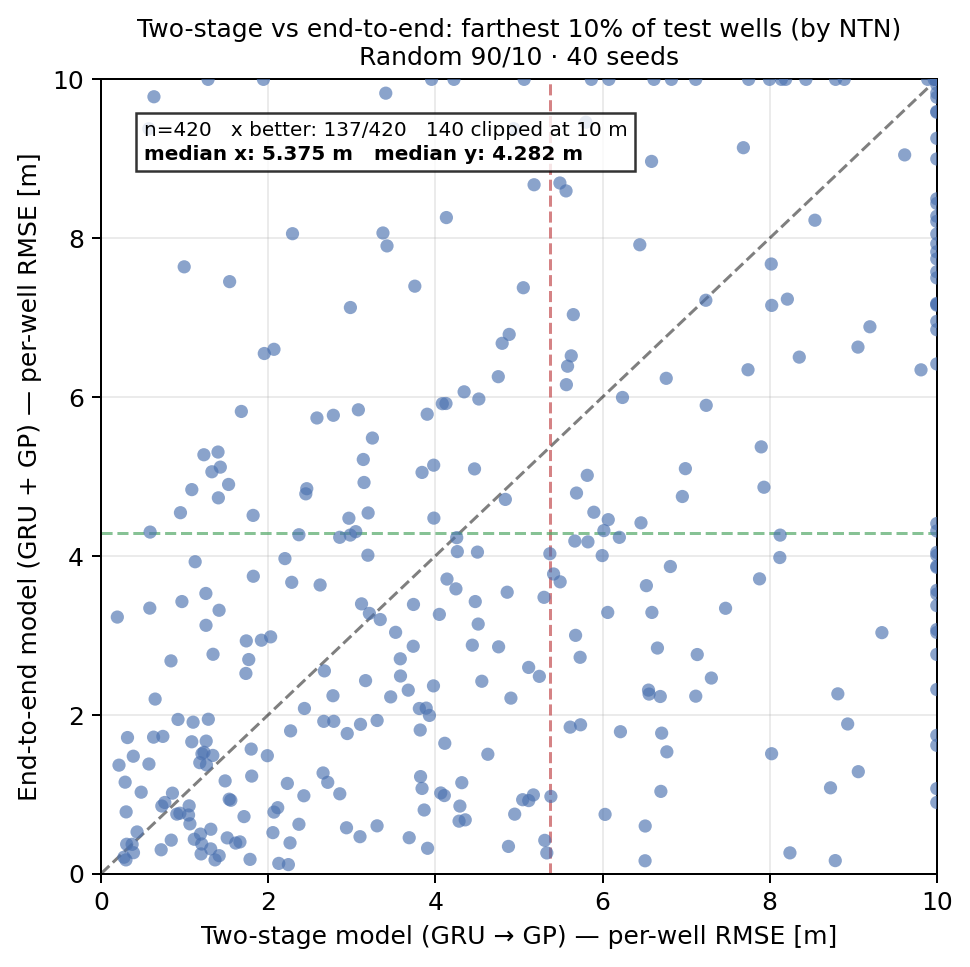
\includegraphics[width=0.47\textwidth]{scatter_main_far}}
  \caption{Per-well RMSE: jointly trained vs.\ two-stage pipeline at the extremes of nearest-training-well distance (random 90/10, 40 seeds)}
\end{figure}

% ============================================================
\section{Alternative Split Strategies}
\label{sec:split_sensitivity}
% ============================================================

The primary evaluation uses the random 90/10 split repeated over 40 seeds. The three alternative
test set configurations described in \cref{sec:alt_splits} are evaluated on the same two-stage spatiotemporal pipeline
to assess whether the choice of split design changes the substantive conclusions.
All three use a 90/10 fraction and are run over 10 seeds.

\begin{table}[htbp]
\centering
\resizebox{\textwidth}{!}{%
\begin{tabular}{lcccc}
\toprule
\textbf{Split strategy} & \textbf{Test wells} & \textbf{avg RMSE (m)} & \textbf{h=16 RMSE (m)} & \textbf{avg IQR-nRMSE} \\
\midrule
random 90/10 (primary, 40 seeds) & 104 & $1.119 \pm 0.208$ & $1.082 \pm 0.193$ & $4.580 \pm 0.909$ \\
Dense-area                       & 104 & $0.678 \pm 0.089$ & $0.681 \pm 0.109$ & $2.900 \pm 0.379$ \\
Sparse-area                      & 104 & $5.102 \pm 0.690$ & $5.409 \pm 0.803$ & $22.269 \pm 3.671$ \\
Cluster-stratified               &  98 & $1.215 \pm 0.202$ & $1.164 \pm 0.220$ & $5.123 \pm 0.973$ \\
Random 80/20                     & 208 & $1.240 \pm 0.154$ & $1.200 \pm 0.142$ & $5.084 \pm 0.586$ \\
\bottomrule
\end{tabular}}
\caption{Two-stage pipeline under alternative split strategies (alternatives: 10 seeds each; primary: 40 seeds; lower is better)}
\label{tab:split_sensitivity}
\end{table}

The Dense-area split achieves substantially lower RMSE than the random split at the same test
fraction (0.678\,m vs.\ 1.119\,m). By restricting the eligible test pool to wells in
the denser half of the monitoring network, the split makes it more likely that test wells have
close training neighbors. The spatial interpolation task is therefore easier by construction.

The Sparse-area split restricts the eligible test pool to the 20\% of wells with the largest
nearest-training-well distances, which are the most spatially isolated wells in the Brandenburg
monitoring network. The two-stage pipeline achieves avg RMSE of $5.102 \pm 0.690$\,m on this
split, roughly $4.6\times$ higher than on the random 90/10 ($1.119$\,m). The jointly trained
pipeline achieves $3.527 \pm 0.406$\,m avg RMSE on the same split, 30.9\% lower. The
ordering from the primary evaluation is reversed, consistent with the distance-binned result in
\cref{sec:joint_results}.

The Cluster-stratified split achieves avg RMSE of $1.215 \pm 0.202$\,m on approximately
98 test wells, 8.6\% higher than the primary random 90/10 split (1.119\,m).

A random 80/20 split (208 test wells, 10 seeds) achieves avg RMSE of $1.240 \pm 0.154$\,m, compared to $1.119 \pm 0.208$\,m for the primary 90/10 split. The larger test fraction places more test wells in sparser parts of the monitoring network, raising error slightly. Full results for all split configurations are in \cref{tab:split_comparison}.

\Cref{fig:split_joint_comparison} shows h=16 RMSE for the two-stage and jointly trained pipelines across all four split designs. For the random 90/10 split, the same 10 seeds (ss42--ss51) are used here as for the three alternative splits, rather than the full 40-seed production run, to keep the seed variance comparable across configurations.

\begin{figure}[htbp]
  \centering
  
\includegraphics[width=0.75\textwidth]{split_strategy_joint_comparison}
  \caption{h=16 RMSE for the two-stage and jointly trained pipelines across four split designs (10 seeds each;
  error bars show $\pm 1$ standard deviation). The jointly trained spatiotemporal model wins only on the Sparse-area split,
  which selects the most spatially isolated test wells.}
  \label{fig:split_joint_comparison}
\end{figure}

% ============================================================
\section{Interpolation Error by Hydrogeological Attributes}
\label{sec:hydrogeo_breakdown}
% ============================================================

This section breaks down interpolation error by three static hydrogeological attributes:
hydrogeological zone, aquifer confinement, and groundwater residence time. All analyses use
the 1{,}040 (well, seed) pairs from the 10-seed random 90/10 split evaluation. A well
appearing in multiple seeds' test sets contributes one pair per seed, because each draw produces a different training set, a different trained model, and therefore different predictions.

\subsection{Hydrogeological Zone}
\label{sec:hydroraum_by_zone}

Brandenburg's monitoring network is partitioned into three zone types: discharge zones
(56\% of pairs), transit zones (36\%), and recharge zones (8\%).
\Cref{tab:hydroraum_breakdown} reports the median RMSE\textsubscript{pw} and the median
nearest-training-well distance for each zone.

\begin{table}[htbp]
\centering
\begin{tabular}{lrrr}
\toprule
\textbf{Zone} & \textbf{Pairs} & \textbf{Median RMSE (m)} & \textbf{Nearest-training-well dist.\ (km)} \\
\midrule
Discharge zones & 583 & 0.636 & 1.609 \\
Transit zones   & 374 & 2.248 & 2.679 \\
Recharge zones  &  83 & 7.972 & 3.387 \\
\bottomrule
\end{tabular}
\caption{Interpolation RMSE by hydrogeological zone}
\label{tab:hydroraum_breakdown}
\end{table}

Discharge zones achieve the lowest median RMSE (0.636\,m) and the shortest median
nearest-training-well distance (1.609\,km). To separate the zone effect from data density,
\cref{tab:hydroraum_dist_matched} subsamples each group by trimming pairs with short nearest-training-well
distances from the bottom of each distribution until the median nearest-training-well distance is nearly equal across zones.

\begin{table}[htbp]
\centering
\begin{tabular}{lrrr}
\toprule
\textbf{Zone} & \textbf{Pairs} & \textbf{Median RMSE (m)} & \textbf{Nearest-training-well dist.\ (km)} \\
\midrule
Discharge zones & 180 & 1.115 & 3.389 \\
Transit zones   & 270 & 2.320 & 3.410 \\
Recharge zones  &  83 & 7.972 & 3.387 \\
\bottomrule
\end{tabular}
\caption{Distance-matched RMSE by hydrogeological zone}
\label{tab:hydroraum_dist_matched}
\end{table}

At matched median nearest-training-well distances, recharge zones are roughly 7$\times$ harder to interpolate
than discharge zones (7.972\,m vs.\ 1.115\,m median RMSE\textsubscript{pw}). Hydrogeological zone thus affects interpolation difficulty beyond what spatial isolation explains.

\subsection{Aquifer Confinement}
\label{sec:confinement_breakdown}

\Cref{tab:confinement_breakdown} splits pairs by aquifer confinement type.

\begin{table}[htbp]
\centering
\begin{tabular}{lrrr}
\toprule
\textbf{Confinement} & \textbf{Pairs} & \textbf{Median RMSE (m)} & \textbf{Nearest-training-well dist.\ (km)} \\
\midrule
Unconfined & 769 & 1.056 & 2.106 \\
Confined   & 271 & 1.005 & 2.113 \\
\bottomrule
\end{tabular}
\caption{Interpolation RMSE by confinement type}
\label{tab:confinement_breakdown}
\end{table}

Median RMSE is nearly identical for unconfined (1.056\,m) and confined (1.005\,m) aquifers
at essentially the same median nearest-training-well distance (2.106\,km vs.\ 2.113\,km). Aquifer
confinement is not a meaningful predictor of interpolation difficulty.

\subsection{Groundwater Residence Time}
\label{sec:residence_time_breakdown}

\Cref{tab:residence_time_breakdown} bins the continuous residence time variable into four
intervals. Of the 1{,}040 pairs, 43 have missing residence time values and are excluded.

\begin{table}[htbp]
\centering
\begin{tabular}{lrrr}
\toprule
\textbf{Residence time} & \textbf{Pairs} & \textbf{Median RMSE (m)} & \textbf{Nearest-training-well dist.\ (km)} \\
\midrule
0--5\,yr   & 299 & 0.759 & 1.946 \\
5--15\,yr  & 417 & 1.057 & 2.171 \\
15--30\,yr & 246 & 1.096 & 2.121 \\
30--50\,yr &  51 & 2.129 & 1.741 \\
\bottomrule
\end{tabular}
\caption{Interpolation RMSE by residence time}
\label{tab:residence_time_breakdown}
\end{table}

Median RMSE increases monotonically with residence time, from 0.759\,m (0--5\,years) to
2.129\,m (30--50\,years). Notably, the 30--50-year bin has the shortest median nearest-training-well distance
(1.741\,km) yet the highest median RMSE. \Cref{tab:residence_time_dist_matched}
subsamples each group to a common median nearest-training-well distance of 2.10\,km (the overall median across
all pairs) to control for this.

\begin{table}[htbp]
\centering
\begin{tabular}{lrrr}
\toprule
\textbf{Residence time} & \textbf{Pairs} & \textbf{Median RMSE (m)} & \textbf{Nearest-training-well dist.\ (km)} \\
\midrule
0--5\,yr   & 283 & 0.766 & 2.104 \\
5--15\,yr  & 401 & 0.970 & 2.101 \\
15--30\,yr & 246 & 1.096 & 2.121 \\
30--50\,yr &  41 & 3.425 & 2.113 \\
\bottomrule
\end{tabular}
\caption{Distance-matched RMSE by residence time}
\label{tab:residence_time_dist_matched}
\end{table}

After distance matching the gradient strengthens: the 30--50-year bin reaches 3.425\,m,
versus 0.766\,m for the 0--5-year bin (4.5$\times$ higher). The residence-time effect is therefore not explained by data density.

% ============================================================
\section{Chapter Summary}
% ============================================================

The results point consistently in one direction: temporal forecast quality is not what limits the spatiotemporal pipeline. Spatial generalization is, and it degrades with distance from the training set. Hydrogeological zone is the only static feature that reliably helps the GP. Joint training does not solve the spatial problem on average but gains an advantage at the extreme tail of spatial isolation. What these findings mean for the forecast-anywhere goal, which approaches failed and why, and where the main gaps are, is the subject of \cref{ch:discussion}.

% Chapter 6 — Discussion
% !TEX root = ../main.tex
% ============================================================
%  Chapter 6 — Discussion
% ============================================================

\chapter{Discussion}
\label{ch:discussion}

\Cref{sec:contributions_discussion} identifies two findings that run through the results: spatial isolation as the primary driver of interpolation difficulty, and the GP as the primary bottleneck. \Cref{sec:protocol_lessons} draws evaluation design lessons, and \cref{sec:dead_ends_section} documents approaches that did not improve results along with the limitations of this work.

% ============================================================
\section{Spatial Isolation and the GP Bottleneck}
\label{sec:contributions_discussion}
% ============================================================

The first finding is that spatial isolation drives interpolation difficulty: seeds and splits that draw spatially isolated test wells produce systematically higher error, and the distance--error relationship holds both across seeds and within seeds, meaning that within any given seed, wells farther from training neighbors also show higher error (\cref{sec:distance_error}). The second is the GP bottleneck: the GRU's temporal predictions at training wells are already accurate enough that substituting them with true observations changes interpolation error by less than 0.003\,m (\cref{sec:bottleneck}), so progress on the forecast-anywhere problem requires better spatial modeling, not a better temporal model.

\subsection{Spatial Isolation Drives Interpolation Difficulty}

Recharge zones are characterized by variable infiltration rates and subsurface properties that produce GWL dynamics that change more sharply over short distances than in discharge zones, where groundwater flows more uniformly, so nearby wells tend to share similar levels. The GP's Mat\'{e}rn-3/2 kernel uses a single smoothness parameter for the whole study area, which means it treats spatial similarity as decaying at the same rate everywhere; recharge zones are where GWL can change sharply over short distances, a pattern a single smoothness parameter cannot fit. Hydrogeological zone works as a GP feature because it groups wells that tend to have similar GWL dynamics, beyond what their location alone would predict. All other tested feature groups either give smaller improvements or even degrade performance relative to the coordinate-only baseline.

\subsection{The GP Bottleneck}

Running 40 split seeds across hundreds of GP configurations would not have been practical with TFT at its training cost; the GRU's speed makes that evaluation affordable. The multi-seed protocol that establishes the distance--error relationship and quantifies seed-to-seed variance is only possible because the temporal backbone is fast enough to run many times. The speedup's main contribution is to evaluation methodology, not to spatial interpolation quality.

\citet{lim2021temporal} show in their ablation that self-attention is among the most important components of TFT. The GRU has no self-attention, yet matches TFT on Brandenburg. This suggests the dataset's smooth seasonal dynamics do not require attention over long time spans.

% ============================================================
\section{Evaluation Design Lessons}
\label{sec:protocol_lessons}
% ============================================================

\subsection{The Co-Location Constraint}

Without the co-location constraint (forcing wells within 8\,m of each other into the training set), the spatiotemporal two-stage pipeline can achieve misleadingly low RMSE on some test wells by effectively copying a co-located training well. The reported metric is dominated by trivially easy cases, not by genuine spatial interpolation. Any spatial evaluation protocol that uses random well splitting without checking for co-located wells may systematically overestimate interpolation performance.

\subsection{Multi-Seed Evaluation and Spatial Composition}

The random split exhibits substantial standard deviation across seeds. The primary cause is that seeds differ in the median distance from test wells to their nearest training neighbor: seeds that draw spatially isolated test wells face a fundamentally harder interpolation problem. This is confirmed by the seed-level analysis in \cref{sec:distance_error}, which shows a positive Spearman correlation ($\rho = 0.603$; \cref{sec:distance_error}) between median nearest-training-well distance and per-seed RMSE. A study relying on a single split seed may therefore report metrics that reflect its spatial composition as much as model quality.

\subsection{Alternative Splits Confirm, Not Replace, the Post-Hoc Distance Analysis}
\label{sec:alt_split_lessons}

The sensitivity analysis in \cref{sec:split_sensitivity} shows that the Dense-area, Sparse-area, and Cluster-stratified splits all reach qualitatively consistent conclusions with the primary random split. Because each alternative split draws a different training set, the results come from independently trained models rather than post-hoc reselections of the random split, which makes the agreement a genuine robustness check. The post-hoc seed analysis on the random split is the more general characterisation, since it spans the full range of spatial configurations rather than fixing difficulty to a chosen range. None of the three alternatives is appropriate as a primary evaluation: the Dense-area split has artificially low RMSE, the Sparse-area split has artificially high RMSE, and the Cluster-stratified split's test-well count is not exactly controllable since cluster sizes are discrete.

% ============================================================
\section{Limitations and Dead Ends}
\label{sec:dead_ends_section}
% ============================================================

\subsection{Negative Results and Dead Ends}
\label{sec:dead_ends}

The following directions do not improve results. They are documented because negative results narrow the hypothesis space and prevent revisiting disproved approaches.

\subsubsection{Residual GP (\texorpdfstring{nRMSE $\approx$ 192}{nRMSE approx 192})}

Training the GP on residuals (the difference between true observations and GRU predictions at training wells) rather than raw GWL values fails completely: nRMSE\textsubscript{pw} $\approx 192$.

GRU prediction errors are not spatially correlated. They are well-specific, as each well has its own dynamics that the global model cannot fully capture (e.g., local recharge anomalies, well-specific seasonal timing). A residual GP therefore fits noise rather than a spatially coherent field and extrapolates that noise catastrophically to test wells.

There is a positive reading of this failure. The GRU's predictions at each well are accurate enough that the residuals show no spatial pattern. If the GRU leaves a systematic trend across locations, a GP could pick that up; since the errors are well-specific rather than regional, the residual GP is just fitting noise.


\subsubsection{Surface Elevation Clipping}

A hypothesis is investigated that clipping GWL predictions to ground surface elevation (GSE, i.e.\ $\hat{y} \leftarrow \min(\hat{y}, \text{GSE})$) might improve performance, since physically the water table cannot rise above the ground surface. Testing GSE clipping on all evaluated model configurations yields $\Delta = 0.000$ in all cases: the model never predicts GWL above the ground surface, so the clipping constraint is never active.

\subsubsection{Depth to Groundwater Table as GP Feature}

Following a suggestion by a collaborator at BGR, depth to the groundwater table (DGT) is tested as an additional GP spatial feature on the random split in a dedicated side experiment; because this experiment is conducted after the main GP feature ablation protocol has been finalized, the result is reported here rather than in \cref{sec:gp_ablation}. DGT alone is harmful (nRMSE\textsubscript{pw} $\approx 8.66$ vs.\ $4.444$ for hydrogeological zone alone); combined with hydrogeological zone it also performs worse than hydrogeological zone alone (nRMSE\textsubscript{pw} $\approx 6.98$ vs.\ $4.444$). DGT does not improve spatial interpolation and is excluded from the selected feature set.

\subsection{Limitations}
\label{sec:limitations}

\paragraph{Hyperparameter search scope.}
Hyperparameters for the GRU and GP are found via iterative grid search. For the jointly trained model, automated HPO with Optuna \citep{akiba2019optuna} finds h128/l5 with coupling weight $\lambda = 0.034$, but a manual architecture sweep shows h256/l4 with $\lambda = 10^{-4}$ gives better interpolation performance. The automated result is unreliable for two reasons: Optuna ran only a limited number of trials, and each trial was evaluated on a single spatial split, where variance is high enough to flip architecture rankings (\cref{sec:seed_design}).

\paragraph{HYRAS reanalysis weather data.}
All experiments use HYRAS~5.0 reanalysis data for the meteorological forcing inputs, including the 16-week forecast horizon. HYRAS~5.0 is a retrospective reconstruction that is available only for the past; it is not a weather forecast. In operational deployment, accurate precipitation and temperature forecasts over 16 weeks are unavailable, and forecast uncertainty would propagate into GWL predictions. The RMSE figures reported here therefore represent an upper bound on achievable performance under perfect meteorological information. The gap between HYRAS-driven and forecast-weather-driven performance is not quantified in this thesis.

\paragraph{GP calibration failure.}
The GP's 95\% nominal prediction intervals achieve only approximately 60\% empirical coverage (mean $0.602 \pm 0.043$ across 40 seeds; Prediction Interval Coverage Probability, PICP) at spatial test wells (production two-stage spatiotemporal pipeline). This is a structural property of GP posterior inference applied to spatial extrapolation: kernel hyperparameters are optimized on training-well data, which may have a different spatial density and correlation structure than the test region. Overconfident here means the kernel-derived posterior intervals are too narrow: the posterior variance is bounded by the output scale $\sigma_f^2$ learned on training data and does not automatically widen for isolated test locations where the actual prediction error exceeds that prior scale. Note that poor coverage is not a direct consequence of poor point predictions: a model with the same NSE but wider uncertainty intervals would still achieve 95\% PICP. The low coverage reflects that the GP underestimates its own uncertainty, which is a separate issue from prediction accuracy.


\paragraph{Static feature availability at genuinely unmonitored locations.}
The GP relies on a single static hydrogeological feature, hydrogeological zone, selected by the feature ablation in \cref{sec:gp_ablation}. Residence time and aquifer confinement are evaluated in the ablation but excluded because both degrade interpolation performance relative to the coordinate-only baseline. At genuinely unmonitored locations (where no well has ever been installed), hydrogeological zone may not be available or may require spatial interpolation from the nearest monitoring records. The accuracy of such interpolated features, and their effect on GP predictions, is not evaluated in this thesis.

\paragraph{Single study area.}
All experiments are conducted exclusively on the Brandenburg LfU monitoring network. The spatial density of this network (1{,}040 wells over 29{,}654\,km$^2$), the hydrogeological diversity of the region, and the HYRAS~5.0 meteorological forcing are specific to this setting. Whether the GRU-GP pipeline and the optimal feature set generalize to other regions, countries, or monitoring densities remains an open question. The pipeline architecture is likely to transfer to other settings, but the feature selection is less certain. Hydrogeological zone works here because it proxies for the spatial correlation structure of GWL dynamics in Brandenburg. In regions where no analogous categorical variable captures that structure, or where GWL dynamics do not follow the same zone pattern, the GP is reduced to coordinate-only interpolation and performance would likely be closer to the coordinate-only baseline in \cref{tab:gp_ablation}.

\paragraph{GRU seed variance not fully characterized.}
The multi-seed evaluation uses a single GRU seed (the best HPO configuration, on the median performing seed out of 10 GRU model seeds) for all spatial interpolation experiments. While GRU performance is stable at this data scale (dominated by split seed variance rather than model initialization), the full sensitivity of the spatial interpolation results to GRU seed choice is not quantified. The same applies to the GP: all spatial experiments use a single GP seed, and sensitivity to GP random initialization is not quantified.

\paragraph{Joint model feature parity.}
The original 40-seed joint runs use 32 GRU static inputs, as hydroraum one-hot features are present in the GP but absent from the GRU, while the two-stage pipeline uses 35. Additional re-runs with matching inputs ($n_\text{static} = 35$) show no meaningful difference (mean $\Delta\text{RMSE}_\text{pw} = -0.011\,\text{m}$, paired $t$-test $p = 0.311$), so the original joint results are valid for comparison.

\paragraph{Joint training per-date batching.}
Both Phase~A and Phase~B of joint training iterate over dates, taking all training wells active on a given date as a batch. Per-date batching is necessary for Phase~B because the GP conditions on all training-well predictions at a single point in time. It is not necessary for Phase~A, which is standard GRU temporal training with no spatial component and could instead use random batching at a larger batch size, as the two-stage GRU does. This would reduce the number of gradient steps per epoch in Phase~A substantially and speed up joint training.

\paragraph{Metric sensitivity.}
All feature comparisons in \cref{sec:gp_ablation} use median per-well nRMSE as the primary criterion because IQR normalization accounts for wells with very different absolute GWL variance. Using per-well RMSE instead could favour different features: a feature that concentrates gains at high-variance wells looks better under nRMSE than under absolute RMSE. This sensitivity between the two metrics is not systematically explored across all feature combinations.

\paragraph{Co-location constraint on alternative splits.}
The alternative split strategies in \cref{sec:split_sensitivity} are also affected by the co-location constraint. Around 30\% of wells are pre-assigned to the training set before any split procedure runs, since co-located pairs always go to training. The pool of wells that the Dense-area, Sparse-area, and Cluster-stratified splits actually operate on is therefore already filtered. Co-located wells make up around 15\% of unique physical locations, so the effect is limited, but all three splits are working from an already-filtered pool, not the full network, which means none of the three split strategies operates on the complete well set as designed.

\paragraph{Limitations of the random split.}
The primary random split is not fully random: the co-location constraint pre-assigns a subset of wells to the training set before random selection runs on the remainder. This is unavoidable unless all but one well per group of co-located wells is dropped, and the effect on aggregate RMSE is small since co-located wells account for a small fraction of unique locations. The reported results should be understood as coming from a random draw over the subset of wells not pre-assigned by the co-location constraint, not the full network.

% ============================================================
\section{Chapter Summary}
% ============================================================

This chapter's two main conclusions are that spatial isolation drives interpolation difficulty and that the GP, not the GRU, is where most of the pipeline's error comes from. Recharge zones are roughly 7$\times$ harder to interpolate than discharge zones at matched distances (\cref{sec:hydroraum_by_zone}). Three evaluation lessons follow: the co-location constraint prevents trivially easy test cases, multi-seed evaluation is necessary because spatial composition dominates variance, and metric choice can reverse feature rankings. None of the dead-end approaches documented here improve on the standard two-stage pipeline, and feature selection is likely less transferable than the pipeline architecture since hydrogeological zone works here because it proxies a spatial correlation structure specific to Brandenburg. The following chapter draws together the main findings and outlines future directions.

% Chapter 7 — Conclusion
% !TEX root = ../main.tex
\chapter{Conclusion}
\label{ch:conclusion}

\section{Summary of Findings}
\label{sec:summary}

This thesis presents GIST (Groundwater Interpolation in Space and Time), a spatiotemporal pipeline for groundwater level forecast interpolation across Brandenburg. The core questions are what limits the pipeline's accuracy and what determines how hard any given prediction is.

A GRU sequence-to-sequence model matches the Temporal Fusion Transformer of \citet{kunz2025} on the Brandenburg dataset, with a median per-well RMSE of 0.088\,m at h\,=\,16 against 0.093\,m for the TFT, at roughly 90$\times$ lower training cost. That speedup makes everything else in this thesis feasible (\cref{tab:pipeline_efficiency}). The hyperparameter optimization, the feature ablation studies, the multi-seed evaluation, and the joint training experiments would all have been impractical at TFT training cost.

The evaluation requires two design choices that turn out to matter. Several wells in the Brandenburg network share identical surface coordinates and are forced into the training set; without this co-location constraint, a random test split can place a test well at the same physical location as a training well, at which point the GP copies a nearby value rather than interpolating, and the measured error does not reflect genuine spatial generalization. The primary evaluation uses a random 90/10 split (104 test wells) repeated over 40 seeds, each drawing a new random 90/10 partition of wells. Running 40 seeds is necessary because seeds differ substantially in how spatially isolated their test wells are, and that isolation is the dominant predictor of per-seed RMSE (\cref{sec:distance_error}).

One of the central findings is about where the bottleneck lies. The two-stage pipeline (GP conditioned on GRU predictions) and a true-observation interpolation baseline (GP conditioned on true observed GWL) differ in per-well RMSE by only 0.003\,m ($p = 0.50$, meaning a difference of this size would arise by chance half the time even if the true gap were zero; \cref{sec:bottleneck}). The GRU's forecast quality is not the limiting factor; the GP's ability to generalize across spatial locations is. At h\,=\,16, the two-stage pipeline achieves a mean per-well RMSE of 1.082\,m, roughly 12$\times$ the GRU's temporal RMSE of 0.088\,m at monitored wells. A systematic GP feature ablation shows that using hydrogeological zone alone is the most beneficial configuration. The reason is visible in per-zone error: at matched nearest-training-well distances, recharge zones are roughly 7$\times$ harder to interpolate than discharge zones (\cref{sec:hydroraum_by_zone}), which means zone membership encodes spatial structure that coordinates alone cannot capture.

The jointly trained model, in which GRU and GP are trained end-to-end with a combined loss, is worse on average ($1.259$\,m vs.\ $1.082$\,m mean per-well RMSE at h\,=\,16). The aggregate hides a distance gradient, though: the two-stage pipeline is better for test wells close to the training network, while the jointly trained model gains an advantage beyond roughly 4.5\,km from the nearest training well. In the Brandenburg monitoring network, most test wells fall within 2\,km of a training neighbor, which is why the aggregate favors the two-stage pipeline. For genuinely isolated locations, the jointly trained model is the stronger choice.

The research question this thesis starts with is whether a dense monitoring network, combined with a spatial interpolation step, can support a forecast-anywhere system. For locations within a few kilometers of the training network, the answer from the Brandenburg data is yes, with median RMSE well under 1\,m for the closest test wells. For genuinely isolated locations the picture is less encouraging: error increases sharply with distance, and joint training only partially closes that gap. Distance to the nearest training well is the dominant constraint, not the quality of the temporal model. The results show what a dense, decades-long monitoring record can achieve and where the hard limits are. Getting reliable predictions far from any monitoring well is still an open problem, and the directions in \cref{sec:future_work} are where that work is most likely to advance. Across most of Brandenburg, monitoring wells are close enough that reliable forecasts are already achievable at the distances reported here. Where monitoring is genuinely sparse, the distance-error relationship quantified in this thesis provides a direct basis for prioritizing where new monitoring infrastructure would reduce forecast uncertainty most.

\section{Future Work}
\label{sec:future_work}

\paragraph{Neural Processes for end-to-end spatiotemporal modeling.}
The two-stage spatiotemporal pipeline separates temporal and spatial learning by design. Convolutional
Conditional Neural Processes \citep{gordon2020convolutional} and related architectures can predict at any new location given a set of observed wells as context, without separating temporal and spatial learning into two stages. These represent the
most principled alternative to the two-stage approach and should be evaluated on the same
Brandenburg test set protocol.

\paragraph{Multi-GRU-seed evaluation.}
The current evaluation uses a single GRU seed. Including three to five GRU seeds in the full
40-seed spatial evaluation matrix would fully characterize the relative contributions of
temporal model variance and spatial split variance to the reported uncertainty.

\paragraph{Multi-seed hyperparameter optimization.}
Hyperparameter search in this thesis uses single-seed evaluations, which have high variance due to the spatial-split sensitivity documented in \cref{sec:seed_design}. Running each trial over multiple spatial splits would reduce that noise and produce a more reliable ranking between candidate architectures. However, because the dominant bottleneck is GP spatial generalization rather than GRU model capacity, better hyperparameter search is unlikely to substantially improve end-to-end interpolation error; the main benefit would be methodological, not a path to dramatically lower RMSE. The same applies to the GP and to the jointly trained model's hyperparameter search. For joint training specifically, which is the component where performance remains furthest behind, improved HPO may offer more practical improvement than refining the GRU configuration further.

\paragraph{Improved joint training architecture.}
The joint training experiment adapts the two-stage architecture for end-to-end training rather than designing a new architecture from scratch. The two-stage pipeline outperforms it at most distances, and an architecture designed from scratch for joint training might narrow that gap.

\paragraph{Generalization to other monitoring networks.}
All results are derived from a single study area. Replication on other dense groundwater
monitoring networks (e.g., the Netherlands Grondwaterregister, the USGS groundwater
monitoring network, or the monitoring networks of other German states) would test whether the optimal GP feature set and the interpolation baseline gap magnitude
are specific to Brandenburg's hydrogeology or are transferable.

\paragraph{Integration of physically derived spatial features.}
The GP relies on a single static feature, hydrogeological zone, selected by the feature ablation in \cref{sec:gp_ablation}. At genuinely unmonitored locations, hydrogeological zone may not be available at the required spatial resolution and would need to be interpolated from regional geological maps. Quantifying how such interpolated zone assignments affect GP predictions is a necessary step toward deployment at locations with no monitoring record.

\paragraph{Removing per-well normalization.}
The pipeline z-scores each well before training, which makes the GP responsible for reconstructing the spatial mean at test locations (\cref{sec:variation}). \citet{kunz2025} skip this step and use GWL standard deviation as a static input instead. Whether the GIST pipeline works better without per-well normalization is a straightforward ablation to run.

\paragraph{Spatial block holdout for stricter generalization testing.}
The split strategies evaluated in this thesis draw test wells from the full monitoring network. A harder test would hold out all wells within a contiguous geographic subregion, with no training wells present in that region. Spatial block cross-validation of this kind is the recommended approach for evaluating spatial models when autocorrelation would otherwise inflate apparent performance \citep{roberts2017cross}, and applying it here would assess whether the GRU-GP pipeline generalizes to areas beyond its training region boundaries rather than interpolating between scattered training wells.

\paragraph{Co-located well selection.}
Right now all co-located wells are forced into training to avoid trivially easy or misleadingly hard test cases (\cref{sec:deduplication}). Keeping only the topmost well from each co-located group eligible for the test set would expand the test pool at the cost of a small reduction in training data, without reintroducing those problems.

\paragraph{Operational weather inputs and forecast uncertainty.}
All experiments in this thesis use HYRAS~5.0 reanalysis weather data, which is available only retrospectively. In an operational deployment, precipitation and temperature forecasts over 16 weeks carry substantial uncertainty. Quantifying how that uncertainty propagates into GWL predictions, and whether it changes the relative ranking of the pipeline configurations, is a necessary step toward actual deployment.

\paragraph{GP uncertainty calibration.}
The GP's 95\% prediction intervals achieve only approximately 60\% empirical coverage (PICP) at spatial test wells, reflecting that the GP underestimates its own uncertainty rather than making poor point predictions. Improving this is important if the pipeline is used for risk assessment or decision support rather than point forecasting alone. Spatially adaptive kernels that account for local differences in monitoring density between training and test regions are a natural starting point.

\paragraph{Empirical Bayesian kriging.}
\citet{zowam2024} replace a global variogram with a local estimate fitted around each prediction point, reducing sensitivity to the stationarity assumption. Adapting this to the GP stage could improve interpolation in regions where the spatial covariance structure differs from the network-wide average, given that zone-specific error varies by nearly an order of magnitude (\cref{sec:hydroraum_by_zone}).


% ---- Bibliography ----
\printbibliography

% ---- Appendix ----
\appendix
% !TEX root = ../main.tex
\chapter{Hyperparameter Configurations}
\label{app:hyperparameters}

\section{Best GRU Configuration (Two-Stage Spatiotemporal Pipeline)}
\label{app:gru_hpo}

\begin{table}[htbp]
\centering
\begin{tabular}{ll}
\toprule
\textbf{Hyperparameter} & \textbf{Value} \\
\midrule
Hidden dimension        & 256 \\
Number of layers        & 4 \\
Dropout                 & 0.2 \\
Learning rate           & $2 \times 10^{-4}$ \\
Batch size              & 4096 \\
Training epochs         & 50 \\
Early stopping patience & 5 \\
Input window length     & 52 weeks \\
Output horizon          & 16 weeks \\
\bottomrule
\end{tabular}
\end{table}

\section{Best GP Configuration (Two-Stage Spatiotemporal Pipeline)}
\label{app:gp_hpo}

\begin{table}[htbp]
\centering
\begin{tabular}{ll}
\toprule
\textbf{Hyperparameter} & \textbf{Value} \\
\midrule
Kernel                  & Matérn-3/2, ARD length-scales \\
Inference               & Exact (Cholesky factorization) \\
Mean function           & Zero \\
GP features             & Hydrogeological zone \\
GP pretraining          & 128 randomly sampled points (all dates, grouped per horizon) \\
Kernel optimization     & 300 gradient-descent steps on marginal log-likelihood \\
GP conditioning dates   & All test-period dates \\
\bottomrule
\end{tabular}
\end{table}

\clearpage
\section{Best Jointly Trained Spatiotemporal Model Configuration}
\label{app:joint_hpo}

\begin{table}[htbp]
\centering
\begin{tabular}{ll}
\toprule
\textbf{Hyperparameter} & \textbf{Value} \\
\midrule
GRU hidden / layers     & 256 / 4 \\
GRU dropout             & 0.2 \\
Learning rate           & $2 \times 10^{-4}$ \\
Batch size              & per-date \\
Early stopping patience & 15 \\
GP loss weight $\lambda$  & $1 \times 10^{-4}$ \\
GP conditioning dates   & all test-period dates \\
\bottomrule
\end{tabular}
\end{table}

% !TEX root = ../main.tex
\chapter{Extended Ablation Results}
\label{app:ablations}

\section{GP Feature Ablation Results}
\label{app:interp_baseline_ablation}

All 30 configurations sorted by nRMSE\textsubscript{pw}.
The selected configuration (hydrogeological zone only) is marked with a star.

\begin{longtable}{p{0.56\linewidth}rrr}
\caption{GP feature ablation: all 30 configurations sorted by
  nRMSE\textsubscript{pw} (median per well, mean over 10 split seeds, 1 GP seed; random 90/10 split;
  coordinate-only baseline nRMSE\textsubscript{pw}\,=\,5.077,
  RMSE\textsubscript{pw}\,=\,1.130\,m)}
\label{tab:gp_ablation_full}\\
\toprule
\textbf{Feature configuration} & \textbf{nRMSE\textsubscript{pw}} &
  \textbf{$\Delta$ nRMSE} & \textbf{RMSE\textsubscript{pw} (m)} \\
\midrule
\endfirsthead
\toprule
\textbf{Feature configuration} & \textbf{nRMSE\textsubscript{pw}} &
  \textbf{$\Delta$ nRMSE} & \textbf{RMSE\textsubscript{pw} (m)} \\
\midrule
\endhead
\midrule
\multicolumn{4}{r}{\footnotesize\itshape (continued on next page)}\\
\endfoot
\bottomrule
\endlastfoot
\textbf{Hydrogeological zone only} $\star$ & \textbf{4.444} & $-$0.633 & \textbf{1.052} \\
Screen top depth only                      & 4.883 & $-$0.194 & 1.070 \\
Screen bottom depth only                   & 4.889 & $-$0.188 & 1.075 \\
Both screen depths                         & 4.906 & $-$0.170 & 1.072 \\
Confinement only                           & 5.017 & $-$0.060 & 1.148 \\
\textit{Spatial coordinates only (baseline)} & 5.077 & ---    & 1.130 \\
Residence time + hydrogeological zone      & 5.118 & $+$0.041 & 1.198 \\
GWL class only                             & 5.155 & $+$0.078 & 1.256 \\
Hydrogeological zone + confinement         & 5.207 & $+$0.130 & 1.153 \\
52-week precipitation lag only             & 5.392 & $+$0.316 & 1.267 \\
Residence time only                        & 5.437 & $+$0.361 & 1.261 \\
Residence time + confinement               & 5.481 & $+$0.404 & 1.315 \\
ACF class only                             & 5.735 & $+$0.658 & 1.332 \\
Residence time + both screen depths        & 5.794 & $+$0.717 & 1.444 \\
Residence time + screen bottom             & 5.800 & $+$0.723 & 1.442 \\
Residence time + screen top                & 5.800 & $+$0.723 & 1.453 \\
Residence time + hydro-zone + confinement  & 5.863 & $+$0.786 & 1.357 \\
52-week precipitation cross-corr only      & 6.040 & $+$0.963 & 1.473 \\
1-week precipitation lag only              & 6.126 & $+$1.049 & 1.278 \\
Res.\ time + hydro-zone + confinement + screen bottom  & 6.193 & $+$1.116 & 1.454 \\
Res.\ time + hydro-zone + confinement + both screen depths & 6.226 & $+$1.149 & 1.430 \\
Res.\ time + hydro-zone + confinement + screen top     & 6.267 & $+$1.190 & 1.427 \\
Res.\ time + hydro-zone + confinement + GWL class (one-hot) & 6.443 & $+$1.366 & 1.586 \\
Res.\ time + hydro-zone + confinement + GWL class (cont.) & 6.598 & $+$1.521 & 1.595 \\
Res.\ time + hydro-zone + confinement + 52w precip lag    & 6.791 & $+$1.714 & 1.616 \\
Residence time + ACF class                 & 6.800 & $+$1.723 & 1.624 \\
Res.\ time + hydro-zone + confinement + 52w precip xcorr  & 6.901 & $+$1.824 & 1.726 \\
Res.\ time + hydro-zone + confinement + ACF class         & 6.903 & $+$1.826 & 1.643 \\
Res.\ time + hydro-zone + confinement + 1w precip lag     & 6.950 & $+$1.873 & 1.548 \\
Res.\ time + hydro-zone + confinement + all precip        & 7.350 & $+$2.273 & 1.815 \\
\end{longtable}

% ============================================================
\section{Spatial Split Comparison}
\label{app:split_comparison}

\begin{table}[htbp]
\centering
\resizebox{\textwidth}{!}{%
\begin{tabular}{lrrrrr}
\toprule
\textbf{Metric}
  & \textbf{Dense-area} & \textbf{Cluster-stratified} & \textbf{Sparse-area}
  & \textbf{Random 90/10}$^\star$ & \textbf{Random 80/20} \\
\midrule
Test wells & 104 & 98 & 104 & 104 & 208 \\
Seeds      & 10  & 10 & 10  & 40  & 10  \\[3pt]
avg RMSE\textsubscript{pw} (m)
  & $0.678 \pm 0.089$ & $1.215 \pm 0.202$ & $5.102 \pm 0.690$
  & $\mathbf{1.119 \pm 0.208}$ & $1.240 \pm 0.154$ \\
h\,=\,16 RMSE\textsubscript{pw} (m)
  & $0.681 \pm 0.109$ & $1.164 \pm 0.220$ & $5.409 \pm 0.803$
  & $\mathbf{1.082 \pm 0.193}$ & $1.200 \pm 0.142$ \\
avg nRMSE\textsubscript{pw}
  & $2.900 \pm 0.379$ & $5.123 \pm 0.973$ & $22.269 \pm 3.671$
  & $\mathbf{4.580 \pm 0.909}$ & $5.084 \pm 0.586$ \\
h\,=\,16 nRMSE\textsubscript{pw}
  & $2.755 \pm 0.329$ & $4.749 \pm 0.964$ & $23.064 \pm 5.054$
  & $\mathbf{4.399 \pm 0.988}$ & $4.798 \pm 0.541$ \\
avg NSE\textsubscript{pw}
  & $-13.5 \pm 3.2$ & $-42.8 \pm 18.1$ & $-878.9 \pm 262.1$
  & $\mathbf{-38.4 \pm 16.9}$ & $-45.4 \pm 14.1$ \\
\bottomrule
\multicolumn{6}{l}{\footnotesize $\star$ Primary evaluation (40 seeds, hydrogeological zone GP features). All other rows: GRU seed 40, GP seed 1.} \\
\end{tabular}}
\caption{Two-stage pipeline across split strategies, f\,=\,0.90}
\label{tab:split_comparison}
\end{table}

% ============================================================
\clearpage
\section{Additional Tables}
\label{app:additional_tables}

\begin{table}[htbp]
\centering
\resizebox{\textwidth}{!}{%
\begin{tabular}{lccc}
\toprule
\textbf{Split seed} & \textbf{Interp.\ Baseline RMSE\textsubscript{pw} (m)} & \textbf{Two-Stage RMSE\textsubscript{pw} (m)} & \textbf{Gap (m)} \\
\midrule
ss42 & 1.127 & 1.122 & $-0.005$ \\
ss43 & 1.021 & 0.998 & $-0.023$ \\
ss44 & 1.162 & 1.126 & $-0.036$ \\
ss45 & 0.974 & 1.014 & $+0.039$ \\
ss46 & 0.818 & 0.827 & $+0.009$ \\
ss47 & 1.029 & 1.048 & $+0.019$ \\
ss48 & 1.045 & 1.050 & $+0.005$ \\
ss49 & 1.420 & 1.380 & $-0.040$ \\
ss50 & 1.001 & 1.063 & $+0.062$ \\
ss51 & 0.842 & 0.808 & $-0.034$ \\
ss52 & 1.138 & 1.159 & $+0.021$ \\
ss53 & 1.302 & 1.338 & $+0.036$ \\
ss54 & 1.212 & 1.223 & $+0.011$ \\
ss55 & 1.124 & 1.118 & $-0.007$ \\
ss56 & 0.872 & 0.905 & $+0.033$ \\
ss57 & 0.913 & 0.918 & $+0.006$ \\
ss58 & 1.025 & 1.046 & $+0.020$ \\
ss59 & 1.314 & 1.301 & $-0.013$ \\
ss60 & 1.375 & 1.366 & $-0.008$ \\
ss61 & 1.120 & 1.123 & $+0.004$ \\
ss62 & 0.934 & 0.896 & $-0.038$ \\
ss63 & 1.385 & 1.352 & $-0.032$ \\
ss64 & 1.060 & 1.068 & $+0.008$ \\
ss65 & 0.896 & 0.909 & $+0.013$ \\
ss66 & 1.224 & 1.270 & $+0.046$ \\
ss67 & 0.751 & 0.751 & $+0.000$ \\
ss68 & 1.131 & 1.136 & $+0.005$ \\
ss69 & 1.060 & 1.050 & $-0.011$ \\
ss70 & 1.268 & 1.281 & $+0.013$ \\
ss71 & 1.182 & 1.191 & $+0.010$ \\
ss72 & 0.975 & 0.934 & $-0.041$ \\
ss73 & 1.601 & 1.617 & $+0.017$ \\
ss74 & 0.890 & 0.937 & $+0.047$ \\
ss75 & 1.228 & 1.102 & $-0.125$ \\
ss76 & 1.195 & 1.213 & $+0.017$ \\
ss77 & 0.827 & 0.847 & $+0.020$ \\
ss78 & 1.020 & 0.999 & $-0.021$ \\
ss79 & 1.593 & 1.597 & $+0.005$ \\
ss80 & 1.478 & 1.518 & $+0.040$ \\
ss81 & 1.096 & 1.140 & $+0.045$ \\
\midrule
Mean & 1.116 & 1.119 & $+0.003$ \\
Std  & 0.208 & 0.208 & 0.033 \\
\bottomrule
\end{tabular}}
\caption{Per-seed interp.\ baseline vs.\ two-stage RMSE\textsubscript{pw}, rand 90/10}
\label{tab:per_seed_trueobs_f90}
\end{table}

\begin{table}[htbp]
\centering
\resizebox{\textwidth}{!}{%
\begin{tabular}{lrrrr}
\toprule
\textbf{Split seed}
  & \textbf{avg RMSE\textsubscript{pw} (m)} & \textbf{h\,=\,16 RMSE\textsubscript{pw} (m)}
  & \textbf{avg NSE\textsubscript{pw}} & \textbf{h\,=\,16 NSE\textsubscript{pw}} \\
\midrule
ss42 & 1.122 & 1.128 & $-31.5$ & $-23.0$ \\
ss43 & 0.998 & 0.974 & $-21.9$ & $-19.7$ \\
ss44 & 1.126 & 1.057 & $-44.1$ & $-41.1$ \\
ss45 & 1.014 & 1.117 & $-40.7$ & $-23.5$ \\
ss46 & 0.827 & 0.912 & $-33.7$ & $-23.4$ \\
ss47 & 1.048 & 1.065 & $-46.4$ & $-30.6$ \\
ss48 & 1.050 & 0.918 & $-31.5$ & $-16.8$ \\
ss49 & 1.380 & 1.251 & $-38.6$ & $-32.5$ \\
ss50 & 1.063 & 1.000 & $-31.2$ & $-32.7$ \\
ss51 & 0.808 & 0.846 & $-29.7$ & $-29.2$ \\
ss52 & 1.159 & 1.129 & $-45.7$ & $-38.6$ \\
ss53 & 1.338 & 1.340 & $-48.6$ & $-47.4$ \\
ss54 & 1.223 & 1.071 & $-25.5$ & $-18.6$ \\
ss55 & 1.118 & 1.157 & $-34.4$ & $-42.2$ \\
ss56 & 0.905 & 0.887 & $-15.2$ & $-13.5$ \\
ss57 & 0.918 & 0.858 & $-22.1$ & $-18.1$ \\
ss58 & 1.046 & 1.053 & $-33.5$ & $-33.1$ \\
ss59 & 1.301 & 1.089 & $-30.0$ & $-31.5$ \\
ss60 & 1.366 & 1.240 & $-42.8$ & $-30.9$ \\
ss61 & 1.123 & 1.223 & $-32.8$ & $-34.2$ \\
ss62 & 0.896 & 0.828 & $-19.2$ & $-15.8$ \\
ss63 & 1.352 & 1.313 & $-72.2$ & $-54.3$ \\
ss64 & 1.068 & 1.101 & $-40.0$ & $-27.5$ \\
ss65 & 0.909 & 0.902 & $-21.0$ & $-18.5$ \\
ss66 & 1.270 & 1.186 & $-43.1$ & $-35.8$ \\
ss67 & 0.751 & 0.742 & $-18.3$ & $-13.9$ \\
ss68 & 1.136 & 1.153 & $-31.4$ & $-24.5$ \\
ss69 & 1.050 & 0.986 & $-27.2$ & $-20.5$ \\
ss70 & 1.281 & 1.204 & $-49.9$ & $-48.0$ \\
ss71 & 1.191 & 1.202 & $-50.3$ & $-42.7$ \\
ss72 & 0.934 & 0.912 & $-25.6$ & $-26.8$ \\
ss73 & 1.617 & 1.496 & $-72.7$ & $-73.4$ \\
ss74 & 0.937 & 0.790 & $-26.6$ & $-21.2$ \\
ss75 & 1.102 & 1.049 & $-52.4$ & $-43.3$ \\
ss76 & 1.213 & 1.128 & $-32.3$ & $-24.1$ \\
ss77 & 0.847 & 0.846 & $-32.6$ & $-30.0$ \\
ss78 & 0.999 & 0.919 & $-21.1$ & $-18.8$ \\
ss79 & 1.597 & 1.511 & $-75.6$ & $-62.7$ \\
ss80 & 1.518 & 1.536 & $-92.6$ & $-92.3$ \\
ss81 & 1.140 & 1.159 & $-50.2$ & $-41.2$ \\
\midrule
Mean & 1.119 & 1.082 & $-38.4$ & $-32.9$ \\
Std  & 0.208 & 0.193 & 16.9    & 16.4    \\
\bottomrule
\end{tabular}}
\caption{Two-stage pipeline per-seed metrics, rand 90/10}
\label{tab:per_seed_two_stage}
\end{table}

\begin{table}[htbp]
\centering
\resizebox{\textwidth}{!}{%
\begin{tabular}{lrrrr}
\toprule
\textbf{Split seed}
  & \textbf{avg RMSE\textsubscript{pw} (m)} & \textbf{h\,=\,16 RMSE\textsubscript{pw} (m)}
  & \textbf{avg NSE\textsubscript{pw}} & \textbf{h\,=\,16 NSE\textsubscript{pw}} \\
\midrule
ss42 & 1.127 & 1.101 & $-32.7$ & $-19.5$ \\
ss43 & 1.021 & 1.008 & $-22.7$ & $-19.5$ \\
ss44 & 1.162 & 1.049 & $-45.2$ & $-35.8$ \\
ss45 & 0.974 & 1.135 & $-42.9$ & $-27.3$ \\
ss46 & 0.818 & 0.883 & $-30.4$ & $-25.1$ \\
ss47 & 1.029 & 1.008 & $-46.4$ & $-30.9$ \\
ss48 & 1.045 & 0.892 & $-31.5$ & $-16.4$ \\
ss49 & 1.420 & 1.248 & $-39.9$ & $-32.5$ \\
ss50 & 1.001 & 0.967 & $-35.1$ & $-30.9$ \\
ss51 & 0.842 & 0.875 & $-30.4$ & $-29.1$ \\
ss52 & 1.138 & 1.136 & $-44.6$ & $-36.0$ \\
ss53 & 1.302 & 1.317 & $-48.3$ & $-47.9$ \\
ss54 & 1.212 & 1.099 & $-26.1$ & $-18.6$ \\
ss55 & 1.124 & 1.148 & $-36.6$ & $-42.1$ \\
ss56 & 0.872 & 0.860 & $-15.4$ & $-12.8$ \\
ss57 & 0.913 & 0.852 & $-22.3$ & $-18.7$ \\
ss58 & 1.025 & 1.041 & $-31.9$ & $-31.2$ \\
ss59 & 1.314 & 1.092 & $-27.9$ & $-28.1$ \\
ss60 & 1.375 & 1.244 & $-41.6$ & $-34.5$ \\
ss61 & 1.120 & 1.209 & $-32.2$ & $-31.8$ \\
ss62 & 0.934 & 0.853 & $-19.0$ & $-15.3$ \\
ss63 & 1.385 & 1.358 & $-74.9$ & $-61.5$ \\
ss64 & 1.060 & 1.085 & $-39.6$ & $-29.2$ \\
ss65 & 0.896 & 0.865 & $-21.0$ & $-18.3$ \\
ss66 & 1.224 & 1.210 & $-42.7$ & $-38.0$ \\
ss67 & 0.751 & 0.734 & $-19.7$ & $-12.7$ \\
ss68 & 1.131 & 1.170 & $-32.2$ & $-24.0$ \\
ss69 & 1.060 & 1.008 & $-27.7$ & $-22.3$ \\
ss70 & 1.268 & 1.184 & $-51.3$ & $-50.8$ \\
ss71 & 1.182 & 1.145 & $-48.6$ & $-41.1$ \\
ss72 & 0.975 & 0.968 & $-25.2$ & $-25.2$ \\
ss73 & 1.601 & 1.514 & $-69.8$ & $-72.3$ \\
ss74 & 0.890 & 0.825 & $-26.4$ & $-22.7$ \\
ss75 & 1.228 & 1.128 & $-53.3$ & $-49.9$ \\
ss76 & 1.195 & 1.125 & $-31.8$ & $-24.8$ \\
ss77 & 0.827 & 0.841 & $-34.1$ & $-30.1$ \\
ss78 & 1.020 & 0.893 & $-20.8$ & $-20.0$ \\
ss79 & 1.593 & 1.476 & $-76.0$ & $-64.6$ \\
ss80 & 1.478 & 1.511 & $-95.6$ & $-92.4$ \\
ss81 & 1.096 & 1.084 & $-50.6$ & $-41.6$ \\
\midrule
Mean & 1.116 & 1.079 & $-38.6$ & $-33.1$ \\
Std  & 0.208 & 0.191 & 17.1    & 16.9    \\
\bottomrule
\end{tabular}}
\caption{True-observation interpolation baseline per-seed metrics, rand 90/10}
\label{tab:per_seed_trueobs}
\end{table}

\begin{table}[htbp]
\centering
\resizebox{\textwidth}{!}{%
\begin{tabular}{lrrrr}
\toprule
\textbf{Split seed}
  & \textbf{avg RMSE\textsubscript{pw} (m)} & \textbf{h\,=\,16 RMSE\textsubscript{pw} (m)}
  & \textbf{avg NSE\textsubscript{pw}} & \textbf{h\,=\,16 NSE\textsubscript{pw}} \\
\midrule
ss42 & 1.088 & 1.053 & $-35.0$ & $-32.9$ \\
ss43 & 1.406 & 1.379 & $-41.4$ & $-39.2$ \\
ss44 & 1.134 & 1.133 & $-48.7$ & $-38.7$ \\
ss45 & 1.149 & 1.132 & $-36.6$ & $-30.8$ \\
ss46 & 1.199 & 1.340 & $-46.6$ & $-52.5$ \\
ss47 & 1.070 & 1.062 & $-41.8$ & $-31.8$ \\
ss48 & 0.976 & 0.903 & $-27.3$ & $-25.9$ \\
ss49 & 1.378 & 1.046 & $-65.4$ & $-42.4$ \\
ss50 & 0.946 & 1.038 & $-24.4$ & $-21.6$ \\
ss51 & 1.163 & 1.119 & $-42.2$ & $-43.8$ \\
ss52 & 1.195 & 1.163 & $-53.8$ & $-43.3$ \\
ss53 & 1.563 & 1.748 & $-80.8$ & $-81.0$ \\
ss54 & 1.522 & 1.586 & $-56.4$ & $-53.3$ \\
ss55 & 1.140 & 0.995 & $-30.5$ & $-26.7$ \\
ss56 & 1.065 & 0.996 & $-16.9$ & $-13.9$ \\
ss57 & 1.007 & 1.093 & $-26.9$ & $-21.1$ \\
ss58 & 0.976 & 0.881 & $-21.3$ & $-17.9$ \\
ss59 & 1.224 & 1.276 & $-42.0$ & $-43.2$ \\
ss60 & 1.495 & 1.393 & $-49.9$ & $-45.4$ \\
ss61 & 1.613 & 1.647 & $-47.0$ & $-51.0$ \\
ss62 & 1.090 & 1.134 & $-45.5$ & $-39.6$ \\
ss63 & 1.361 & 1.125 & $-61.6$ & $-43.0$ \\
ss64 & 1.604 & 1.532 & $-82.6$ & $-73.9$ \\
ss65 & 1.427 & 1.364 & $-69.1$ & $-59.8$ \\
ss66 & 1.549 & 1.535 & $-44.6$ & $-40.5$ \\
ss67 & 1.072 & 1.122 & $-28.8$ & $-30.3$ \\
ss68 & 1.157 & 1.013 & $-35.2$ & $-26.5$ \\
ss69 & 1.290 & 1.324 & $-51.7$ & $-43.7$ \\
ss70 & 1.587 & 1.585 & $-61.3$ & $-52.8$ \\
ss71 & 1.158 & 1.038 & $-42.9$ & $-39.0$ \\
ss72 & 1.150 & 1.193 & $-50.0$ & $-48.7$ \\
ss73 & 1.702 & 1.716 & $-100.3$ & $-86.3$ \\
ss74 & 1.008 & 1.069 & $-33.1$ & $-21.4$ \\
ss75 & 1.377 & 1.390 & $-86.0$ & $-77.6$ \\
ss76 & 1.582 & 1.177 & $-60.6$ & $-37.2$ \\
ss77 & 1.202 & 1.212 & $-47.0$ & $-47.1$ \\
ss78 & 0.947 & 0.986 & $-30.1$ & $-25.8$ \\
ss79 & 1.528 & 1.484 & $-67.6$ & $-57.5$ \\
ss80 & 2.319 & 2.347 & $-218.8$ & $-205.2$ \\
ss81 & 1.028 & 1.011 & $-32.7$ & $-30.5$ \\
\midrule
Mean & 1.286 & 1.259 & $-52.1$ & $-46.1$ \\
Std  & 0.278 & 0.290 & 32.8    & 30.8 \\
\bottomrule
\end{tabular}}
\caption{Jointly trained model per-seed metrics, rand 90/10}
\label{tab:per_seed_joint}
\end{table}

\begin{table}[htbp]
\centering
\caption{Joint model $\lambda$ sweep (h256/l4, 1 GP seed)}
\label{tab:lambda_sweep}
\begin{tabular}{lrr}
\toprule
$\boldsymbol{\lambda}$ & \textbf{RMSE\textsubscript{pw} (m)} & \textbf{nRMSE\textsubscript{pw}} \\
\midrule
0.9    & 1.403 & 7.88 \\
0.7    & 1.352 & 8.58 \\
0.5    & 1.255 & 6.27 \\
0.3    & 1.048 & 5.89 \\
0.1    & 1.091 & 5.62 \\
0.01   & 1.115 & 5.42 \\
0.001  & 1.025 & 5.50 \\
\textbf{0.0001} & \textbf{1.016} & \textbf{5.50} \\
0.00001 & 1.348 & 7.22 \\
\bottomrule
\end{tabular}
\end{table}

\begin{table}[htbp]
\centering
\caption{Joint model architecture sweep ($\lambda = 0.034$, 1 GP seed), h256/l4 selected}
\label{tab:arch_sweep}
\begin{tabular}{lcccc}
\toprule
\textbf{Arch} & \textbf{Hidden} & \textbf{Layers} & \textbf{RMSE\textsubscript{pw} (m)} & \textbf{nRMSE\textsubscript{pw}} \\
\midrule
\textbf{h256/l4} & 256 & 4 & \textbf{1.419} & \textbf{7.08} \\
h128/l5          & 128 & 5 & 1.426          & 7.17 \\
\bottomrule
\end{tabular}
\end{table}

\begin{table}[htbp]
\centering
\begin{tabular}{lrr}
\toprule
\textbf{Metric} & \textbf{Two-Stage} & \textbf{Jointly Trained} \\
\midrule
\multicolumn{3}{l}{\textit{Per-well spatial metrics (mean $\pm$ std, 40 seeds)}} \\[2pt]
h\,=\,16 RMSE\textsubscript{pw} (m)        & $1.082 \pm 0.193$ & $1.259 \pm 0.290$ \\
avg RMSE\textsubscript{pw} (m)              & $1.119 \pm 0.208$ & $1.286 \pm 0.278$ \\
avg nRMSE\textsubscript{pw}                 & $4.580 \pm 0.909$ & --- \\
h\,=\,16 NSE\textsubscript{pw}              & $-32.9 \pm 16.4$  & $-46.1 \pm 30.8$ \\
avg NSE\textsubscript{pw}                   & $-38.4 \pm 16.9$  & $-52.1 \pm 32.8$ \\
NSE\textsubscript{pw} P10                   & $-3731 \pm 1858$  & $-3299 \pm 1871$ \\
NSE\textsubscript{pw} P25                   & $-505 \pm 300$    & $-532 \pm 279$ \\
NSE\textsubscript{pw} P75                   & $-3.83 \pm 1.93$  & $-6.49 \pm 4.12$ \\
NSE\textsubscript{pw} P90                   & $-0.221 \pm 0.353$ & $-0.580 \pm 0.804$ \\
RMSE\textsubscript{pw} P10 (m)              & $0.243 \pm 0.036$ & $0.268 \pm 0.051$ \\
RMSE\textsubscript{pw} P25 (m)              & $0.440 \pm 0.071$ & $0.548 \pm 0.131$ \\
RMSE\textsubscript{pw} P50 (m)              & $1.119 \pm 0.208$ & $1.286 \pm 0.278$ \\
RMSE\textsubscript{pw} P75 (m)              & $3.497 \pm 0.740$ & $3.624 \pm 0.826$ \\
RMSE\textsubscript{pw} P90 (m)              & $9.015 \pm 2.382$ & $8.871 \pm 1.974$ \\[3pt]
\multicolumn{3}{l}{\textit{Uncertainty calibration}} \\[2pt]
PICP-95                                     & $0.602 \pm 0.043$ & $0.629 \pm 0.055$ \\[3pt]
\multicolumn{3}{l}{\textit{Global (pooled) metrics}} \\[2pt]
Global RMSE (m)                             & $7.169 \pm 1.502$ & $6.243 \pm 1.258$ \\
Global NSE                                  & $0.917 \pm 0.029$ & $0.937 \pm 0.022$ \\
Global nRMSE                                & $0.219 \pm 0.056$ & $0.192 \pm 0.051$ \\
Global MAE (m)                              & $3.437 \pm 0.635$ & $3.291 \pm 0.557$ \\
Global KGE                                  & $0.909 \pm 0.045$ & $0.927 \pm 0.036$ \\
Abs.\ error P95 (m)                         & $15.43 \pm 3.15$  & $13.60 \pm 3.06$ \\
Abs.\ error P99 (m)                         & $30.82 \pm 9.99$  & $25.64 \pm 8.17$ \\
\bottomrule
\end{tabular}
\caption{Two-stage vs.\ joint: full metrics, rand 90/10}
\label{tab:cross_split_full_metrics}
\end{table}

\begin{table}[htbp]
\centering
\resizebox{\textwidth}{!}{%
\begin{tabular}{lccc}
\toprule
\textbf{Split seed} & \textbf{Nearest-training-well dist.\ (km)} & \textbf{avg RMSE\textsubscript{pw} (m)} & \textbf{h\,=\,16 RMSE\textsubscript{pw} (m)} \\
\midrule
ss62 & 1.718 & 0.896 & 0.828 \\
ss58 & 1.720 & 1.051 & 1.053 \\
ss51 & 1.783 & 0.810 & 0.846 \\
ss67 & 1.806 & 0.750 & 0.742 \\
ss81 & 1.812 & 1.145 & 1.159 \\
ss64 & 1.966 & 1.072 & 1.101 \\
ss56 & 1.974 & 0.911 & 0.887 \\
ss77 & 1.990 & 0.852 & 0.846 \\
ss44 & 1.991 & 1.125 & 1.057 \\
ss57 & 1.997 & 0.918 & 0.858 \\
ss43 & 2.008 & 1.002 & 0.974 \\
ss54 & 2.010 & 1.225 & 1.071 \\
ss65 & 2.020 & 0.910 & 0.902 \\
ss72 & 2.046 & 0.936 & 0.912 \\
ss42 & 2.064 & 1.122 & 1.128 \\
ss45 & 2.080 & 1.017 & 1.117 \\
ss76 & 2.105 & 1.227 & 1.128 \\
ss55 & 2.115 & 1.123 & 1.157 \\
ss59 & 2.139 & 1.303 & 1.089 \\
ss78 & 2.172 & 1.001 & 0.919 \\
ss49 & 2.174 & 1.379 & 1.251 \\
ss50 & 2.183 & 1.063 & 1.000 \\
ss47 & 2.184 & 1.051 & 1.065 \\
ss63 & 2.188 & 1.353 & 1.313 \\
ss69 & 2.203 & 1.048 & 0.986 \\
ss74 & 2.208 & 0.944 & 0.790 \\
ss68 & 2.216 & 1.136 & 1.153 \\
ss80 & 2.231 & 1.519 & 1.536 \\
ss66 & 2.240 & 1.275 & 1.186 \\
ss46 & 2.246 & 0.826 & 0.912 \\
ss48 & 2.257 & 1.051 & 0.918 \\
ss71 & 2.292 & 1.191 & 1.202 \\
ss61 & 2.317 & 1.121 & 1.223 \\
ss75 & 2.323 & 1.105 & 1.049 \\
ss60 & 2.331 & 1.365 & 1.240 \\
ss70 & 2.339 & 1.285 & 1.204 \\
ss73 & 2.352 & 1.627 & 1.496 \\
ss79 & 2.386 & 1.595 & 1.511 \\
ss52 & 2.422 & 1.159 & 1.129 \\
ss53 & 2.537 & 1.337 & 1.340 \\
\midrule
Spearman $\rho$ (dist.\ vs.\ avg RMSE\textsubscript{pw}) & \multicolumn{3}{c}{$0.603$ ($p < 0.001$)} \\
Spearman $\rho$ (dist.\ vs.\ h\,=\,16 RMSE\textsubscript{pw}) & \multicolumn{3}{c}{$0.601$ ($p < 0.001$)} \\
\bottomrule
\multicolumn{4}{l}{\footnotesize $\rho$ computed from full-precision values; displayed distances are rounded to 3\,d.p. All RMSE\textsubscript{pw} values are medians over test wells.} \\
\end{tabular}}
\caption{Per-seed two-stage pipeline RMSE\textsubscript{pw} vs.\ median nearest-training-well distance (random 90/10, 40 seeds, sorted by nearest-training-well distance)}
\label{tab:seed_distance}
\end{table}

\begin{table}[htbp]
\centering
\resizebox{\textwidth}{!}{%
\begin{tabular}{crrrrrr}
\toprule
\textbf{Decile} & \textbf{NTN range (km)} & \textbf{NTN median (km)} & \textbf{$n$ pairs}
  & \textbf{Two-stage median RMSE\textsubscript{pw} (m)} & \textbf{Joint median RMSE\textsubscript{pw} (m)}
  & \textbf{Two-stage wins (\%)} \\
\midrule
D1 (closest) & 0.01--0.61 & 0.394 & 422 & 0.675 & 1.098 & 66.8 \\
D2           & 0.62--0.99 & 0.823 & 420 & 0.566 & 0.909 & 64.5 \\
D3           & 1.00--1.36 & 1.220 & 411 & 0.699 & 0.771 & 60.3 \\
D4           & 1.36--1.72 & 1.570 & 420 & 0.608 & 0.950 & 63.8 \\
D5           & 1.73--2.25 & 2.043 & 414 & 0.725 & 0.860 & 51.4 \\
D6           & 2.25--2.72 & 2.456 & 409 & 0.899 & 0.836 & 51.8 \\
D7           & 2.72--3.36 & 3.036 & 420 & 1.481 & 1.534 & 51.7 \\
D8           & 3.37--4.24 & 3.776 & 413 & 1.853 & 1.953 & 40.2 \\
D9           & 4.24--5.45 & 4.677 & 418 & 2.406 & 2.550 & 45.7 \\
D10 (farthest) & 5.45--21.4 & 6.809 & 413 & 5.369 & 4.261 & 31.7 \\
\bottomrule
\end{tabular}}
\caption{Two-stage vs.\ jointly trained by NTN distance decile}
\label{tab:decile_comparison}
\end{table}


\begin{table}[htbp]
\centering
\caption{Top 5 static features by permutation importance (run 0346, h256/l4, 5 repeats per
feature). Delta is the mean increase in nRMSE\textsubscript{pw} relative to the baseline
(0.0467). All 35 features have positive delta; only the five largest are shown.}
\label{tab:perm_importance}
\begin{tabular}{clrr}
\toprule
\textbf{Rank} & \textbf{Feature} & \textbf{$\Delta$ nRMSE\textsubscript{pw}} & \textbf{\% change} \\
\midrule
1 & Pardé seasonality coefficient        & $+0.0221$ & $+47.3\%$ \\
2 & Water courses fraction               & $+0.0057$ & $+12.3\%$ \\
3 & Topographic Wetness Index            & $+0.0049$ & $+10.5\%$ \\
4 & Surface elevation                    & $+0.0048$ & $+10.2\%$ \\
5 & Pastures fraction                    & $+0.0040$ & $+8.6\%$  \\
\midrule
--- & All remaining 30 features & $+0.001$--$+0.003$ & $+2$--$+7\%$ \\
\bottomrule
\end{tabular}
\end{table}

\begin{table}[htbp]
\centering
\caption{Dynamic covariate permutation importance (run 0346, h256/l4, 5 repeats per
feature). Delta is the mean increase in nRMSE\textsubscript{pw} relative to the baseline
(0.0467).}
\label{tab:perm_importance_dynamic}
\begin{tabular}{clrr}
\toprule
\textbf{Rank} & \textbf{Feature} & \textbf{$\Delta$ nRMSE\textsubscript{pw}} & \textbf{\% change} \\
\midrule
1 & Temperature (5\,km)          & $+0.0428$ & $+91.5\%$ \\
2 & Precipitation (5\,km)        & $+0.0395$ & $+84.5\%$ \\
3 & Calendar cosine encoding     & $+0.0187$ & $+40.0\%$ \\
4 & Relative humidity (5\,km)   & $+0.0099$ & $+21.2\%$ \\
5 & Calendar sine encoding       & $+0.0098$ & $+20.9\%$ \\
\bottomrule
\end{tabular}
\end{table}


% !TEX root = ../main.tex
\chapter{Static Feature Definitions and Model Assignments}
\label{app:features}

\Cref{tab:features_gru,tab:features_gp,tab:features_unused} list all 40 static features
available in the Brandenburg groundwater dataset, grouped by their role in the modelling
pipeline. \textbf{GRU} features are passed as \texttt{x\_static} to the temporal model.
\textbf{GP} features are used as spatial covariates in the Gaussian Process kernel.
Features marked \textbf{---} are available in the dataset but are not primary model inputs
in the main experiments.

\begin{longtable}{p{5.5cm}p{2.5cm}p{5cm}}
\caption{GRU static inputs (35 features). All are standardized before training. The three hydrogeological zone indicators are additionally used as GP spatial inputs (\cref{tab:features_gp}).}
\label{tab:features_gru} \\
\toprule
\textbf{Column name} & \textbf{Group} & \textbf{Description} \\
\midrule
\endfirsthead
\multicolumn{3}{l}{\small\itshape (continued from previous page)} \\
\toprule
\textbf{Column name} & \textbf{Group} & \textbf{Description} \\
\midrule
\endhead
\midrule
\multicolumn{3}{r}{\small\itshape (continued on next page)} \\
\endfoot
\bottomrule
\endlastfoot
\path{corine_1000_fractions_corineclccode_111} & Land use & Continuous urban fabric fraction \\
\path{corine_1000_fractions_corineclccode_112} & Land use & Discontinuous urban fabric fraction \\
\path{corine_1000_fractions_corineclccode_121} & Land use & Industrial/commercial units fraction \\
\path{corine_1000_fractions_corineclccode_131} & Land use & Mineral extraction sites fraction \\
\path{corine_1000_fractions_corineclccode_141} & Land use & Green urban areas fraction \\
\path{corine_1000_fractions_corineclccode_211} & Land use & Non-irrigated arable land fraction \\
\path{corine_1000_fractions_corineclccode_231} & Land use & Pastures fraction \\
\path{corine_1000_fractions_corineclccode_242} & Land use & Complex cultivation patterns fraction \\
\path{corine_1000_fractions_corineclccode_311} & Land use & Broad-leaved forest fraction \\
\path{corine_1000_fractions_corineclccode_312} & Land use & Coniferous forest fraction \\
\path{corine_1000_fractions_corineclccode_313} & Land use & Mixed forest fraction \\
\path{corine_1000_fractions_corineclccode_321} & Land use & Natural grasslands fraction \\
\path{corine_1000_fractions_corineclccode_322} & Land use & Moors and heathland fraction \\
\path{corine_1000_fractions_corineclccode_411} & Land use & Inland marshes fraction \\
\path{corine_1000_fractions_corineclccode_511} & Land use & Water courses fraction \\
\path{corine_1000_fractions_corineclccode_512} & Land use & Water bodies fraction \\
\midrule
\path{TWI_dgm50_r1000m}               & Terrain & Topographic Wetness Index (1\,km buffer) \\
\path{gok}                             & Terrain & Surface elevation (m\,a.s.l.) \\
\midrule
\path{eumohp_1000_mean_dsd1}          & EU-MOHP & Drainage system density, Strahler-1 watercourses \\
\path{eumohp_1000_mean_lp1}           & EU-MOHP & Linear permeability, Strahler-1 \\
\path{eumohp_1000_mean_sd1}           & EU-MOHP & Stream density, Strahler-1 \\
\midrule
\path{amatulli_1000_mean_entgeom10kment}   & Geomorpho90m & Geomorphological entropy (10\,km scale) \\
\path{amatulli_1000_mean_shannongeom10kmsha} & Geomorpho90m & Shannon entropy of terrain (10\,km scale) \\
\path{amatulli_1000_mean_unigeom10kmuni}   & Geomorpho90m & Terrain uniformity (10\,km scale) \\
\midrule
\path{huek250_1000_fractions_kf_9}   & HÜK250 & Hydraulic conductivity class 9 fraction \\
\path{huek250_1000_fractions_kf_10}  & HÜK250 & Hydraulic conductivity class 10 fraction \\
\path{huek250_1000_fractions_kf_11}  & HÜK250 & Hydraulic conductivity class 11 fraction \\
\midrule
\path{gwn1000_1000_mean_recharge}     & GW recharge & Mean annual GW recharge, source 1 (mm/yr) \\
\path{GW_recharge_r1000m}             & GW recharge & Mean annual GW recharge, source 2 (mm/yr) \\
\midrule
\path{parde_seasonality}              & Seasonality & Pardé seasonality coefficient (per-well time series) \\
\path{gw_gespannt_bin}                & Confinement & Aquifer confinement binary (1\,=\,confined) \\
\path{siwa_verweilzeit_j}             & Residence time & GW residence time in years (ordinal: 0,1,3,10,30,50) \\
\midrule
\path{hydroraum_Speisungsgebiete}     & Hydro zone & Recharge zone indicator (binary) \\
\path{hydroraum_Transitgebiete}       & Hydro zone & Transit zone indicator (binary) \\
\path{hydroraum_Entlastungsgebiete}   & Hydro zone & Discharge zone indicator (binary) \\
\end{longtable}

\begin{table}[htbp]
\centering
\caption{GP spatial inputs (3 features). One-hot encoding of hydrogeological zone (\texttt{hydroraum}); also included in the GRU feature set above.}
\label{tab:features_gp}
\small
\begin{tabular}{p{5.5cm}p{2.5cm}p{5cm}}
\toprule
\textbf{Column name} & \textbf{Group} & \textbf{Description} \\
\midrule
\path{hydroraum_Speisungsgebiete}     & Hydro zone & Recharge zone indicator (binary) \\
\path{hydroraum_Transitgebiete}       & Hydro zone & Transit zone indicator (binary) \\
\path{hydroraum_Entlastungsgebiete}   & Hydro zone & Discharge zone indicator (binary) \\
\bottomrule
\end{tabular}
\end{table}

\begin{table}[htbp]
\centering
\caption{Features available in the dataset but not used as primary model inputs.}
\label{tab:features_unused}
\small
\begin{tabular}{p{5.5cm}p{2.5cm}p{5cm}}
\toprule
\textbf{Column name} & \textbf{Group} & \textbf{Description} \\
\midrule
\path{gwlk}     & Aquifer complex & Glacial aquifer complex (3 classes: \emph{Grundwasserleiterkomplexe}) \\
\path{fok}      & Screen depth & Well screen top depth, \emph{Filteroberkante} ($\sim$19\% missing) \\
\path{fuk}      & Screen depth & Well screen bottom depth, \emph{Filterunterkante} ($\sim$19\% missing) \\
\path{acf_class} & ACF & Autocorrelation lag class ($<$6, $<$9, $<$12, $<$20, $<$53, $>$53 weeks); requires historical GWL to compute \\
\path{gw_gespannt} & Confinement & Raw confinement string; replaced by \path{gw_gespannt_bin} \\
\bottomrule
\end{tabular}
\end{table}


\end{document}
